\documentclass[12pt,a4paper,oneside,czech,american]{book} % TODO: Update 'oneside' or 'twoside' - depending on number of pages

%%% Packages:
%% Necessary packages:
\usepackage[T1]{fontenc}		% Font encoding
\usepackage[utf8]{inputenc}		% Input encoding
\usepackage[a4paper, hmarginratio=3:2]{geometry}	% Use of the A4 page and setting the margins (the binding will be wider)

%% Other packages:
% Code:
\usepackage{listings} 			 % Code formatting package

% Fonts:
\usepackage[hidelinks]{hyperref} % Hide square around URL link.
\usepackage{amsmath}  			 % Advanced mathematic package
\usepackage{xcolor}    			 % Colorful text
\usepackage{soul}				 % Text fonts syllable by syllable - used for in-text codifying
\usepackage{amsfonts}			 % Font package permitting the use of \mathbb{}, among other functionalities

% Graphics:
\usepackage{graphicx} 			 % Insert raster graphic files (PNG etc.)
\usepackage{epsfig} 			 % Insert EPS graphics files
\usepackage{float} 			  	 % Advanced figure placement options
\usepackage{caption} 			 % Captions of figures, tables, etc.
\usepackage{subcaption}			 % Sub-captions of figures, tables, etc. 
\usepackage{tikz}				 % Visual representation of matrices, graphs etc.
\usetikzlibrary{plotmarks, positioning}
\usepackage{pgfplots} 			% For visualizations, graphics, etc.
\pgfplotsset{compat=1.3}		% Use pgfplots version 1.3 specifically

% Languages:
\usepackage{babel}

% Page formatting:
% TODO: Replace placeholder PDF with scan of orignal task paper
\usepackage{pdfpages}			 % Add PDFs into compiled PDF

% Tables:
\usepackage{tabularx}			 % Advanced table options
\usepackage{colortbl} 			 % Table cell color

%%% Document settings:
% TODO: Play around with the following if the formatting of pages turns out weird
\widowpenalty=9500 	   % Completely avoid widows (last lines of paragraph on a new page)
\clubpenalty=9500 	   % Completely avoid orphans (first lines of a new paragraph on the bottom of a page)
\brokenpenalty=9500    % Prohibit page breaks after a line that has a split word at the end

\topmargin=-15mm      % Upper edge slightly smaller
\textwidth=150mm      % Text width on the page
\textheight=240mm     % Height of the text on the page

\pagenumbering{arabic} % Page numbering in Arabic numerals
\pagestyle{plain}      % Page numbering at the bottom center

\parindent=0pt 		  % Indentation of the 1st line of the paragraph
\parskip=7pt   		  % Spacing between paragraphs


%%% Custom colors:
\definecolor{nvidia}{rgb}{0.6, 0.73, 0.35}		% Nvidia color
\definecolor{lightnvidia}{rgb}{0.92, 1.0, 0.85} % Nvidia light color
\definecolor{light-gray}{gray}{0.95}			% In-text code highlighting color
\definecolor{lbcolor}{rgb}{0.9,0.9,0.9}			% Code block background color
\definecolor{Darkgreen}{rgb}{0.0, 0.2, 0.13}	% Code block comments color


%%% Custom code block:
\lstset{
	backgroundcolor=\color{lbcolor}, % Background color of the code block
	upquote=true,					 % Format of quote: true -> '', false -> ‘’
	columns=fixed,					 % Characters are below each other (each column is one character -> fixed column size)
	extendedchars=false,			 % Allow national characters, for example, Czech diacritics. If true, then load any package that defines the characters, for example, fontenc, or inputenc, etc.
	showtabs=false,					 % Tabulators visible or not
	showspaces=false,				 % All blank spaces visible as _ or not
	showstringspaces=false,			 % Blank spaces in strings visible as _ or not 
	identifierstyle=\ttfamily,		 % Code font to be monospace if the line begins with one of the following: a-z, A-Z, @, $ and _
	language=C++,					 % Default language syntax highlighting for code blocks
	captionpos=b,					 % Position of the caption. b - bottom; t - top of the listing
	tabsize=2,						 % Set tabulator stops			
	frame=lines,					 % Draw a line on the top and bottom of the code listing -> frame
	numbers=left,					 % Print line numbers on the left of the code block
	numberstyle=\tiny,				 % Font and size of line numbers
	numbersep=5pt,					 % Distance between line numbers and the code block
	basicstyle=\footnotesize,		 % Basic font. Selected at the beginning of each listing
	keywordstyle=\color[rgb]{0,0,1}, % Fond of language keywords in a specific font
	commentstyle=\color{Darkgreen},	 % Font of comments in code block
	stringstyle=\color{red},		 % Font of non-keywords, comments and strings
	breaklines=true,				 % Breaking of long lines
	prebreak = \raisebox{0ex}[0ex][0ex]{\ensuremath{\hookleftarrow}}, % Line-break symbol if a line of code is too long
}
% Extend C++ with CUDA keywords - not supported in lstlisting by default.
\lstset{
	morekeywords={__global__},
	morekeywords={__device__},
	morekeywords={blockDim.x},
	morekeywords={blockDim.y},
	morekeywords={blockIdx.x},
	morekeywords={blockIdx.y},	
	morekeywords={threadIdx.x},
	morekeywords={threadIdx.y},
	morekeywords={gridDim.x},
	morekeywords={__shared__},
	morekeywords={dim3},
	alsoletter={.}				% Make the font be applied for dots
}


%%% Custom commands:
\newcommand{\ti}{\textit} 								  % Shortcut for cursive font
\newcommand{\tb}{\textbf} 								  % Shortcut for bold fond
%\newcommand{\code}[1]{%									  % Shortcut for code font in text
%	\begingroup
%	\sethlcolor{light-gray}%
%	\hl{\texttt{#1}}%
%	\endgroup
%}

\newcommand{\code}[1]{\colorbox{light-gray}{\texttt{#1}}}

%% Status of writing:
\newcommand{\TODO}{\textcolor{red}{TODO}}   		   % To Do command
\newcommand{\ENGLISH}{\textcolor{green}{ENGLISH}}      % Writing To Be Checked by someone who knows English grammar
\newcommand{\TO}{\textcolor{nvidia}{TO}} 				   % Writing To Be Checked by Supervisor (Tomas Oberhuber)


%%% Constants
\newcommand{\cvut}{České vysoké učení technické v Praze}
\newcommand{\fjfi}{Fakulta jaderná a fyzikálně inženýrská}
\newcommand{\ksi}{Katedra softwarového inženýrství}
\newcommand{\programme}{Aplikace přírodních věd}
\newcommand{\specialization}{Aplikace softwarového inženýrství}

\newcommand{\kind}{Výzkumný úkol}

\newcommand{\logoCVUT}{
\includegraphics{images/title/cvut_logo_contour_version.pdf}}

% The following was filled in accordance with the original task paper
\newcommand{\titleCZ}{Paralelní LU rozklad pro GPU}			 % Czech title of the project
\newcommand{\titleEN}{Parallel LU Decomposition for the GPU} % English title of the project
\newcommand{\paperAuthor}{Bc. Lukáš Čejka}   				 % Name and surname, including academic titles
\newcommand{\supervisor}{doc. Ing. Tomáš Oberhuber, Ph.D.} 	 % Name and surname of supervisor, including academic titles
\newcommand{\supervisorWorkspace}{\ksi, \fjfi, \cvut} 			 % Workplace of supervisor

% TODO: Can Klinkovsky be considered a consultant?
\newcommand{\consultant}{--} 								 % Consultant's name, surname and academic titles, if I have a consultant
\newcommand{\consultantWorkspace}{--} 							 % Consultant's workplace, if I have a consultant

\newcommand{\yearSubmitted}{2022}  									 % Year of handing in the thesis (not the academic years)
\newcommand{\place}{Praze} 									 % City of studying

% TODO: Fill in the following at the end
\newcommand{\keywordCZ}{Klíčová slova}   						 % Enter 5 keywords max. in Czech
\newcommand{\keywordEN}{Key words}       						 % Enter 5 keywords max. in English (translations of the Czech keywords)
\newcommand{\abstractCZ}{Popis práce česky}    				 % Abstract in Czech (roughly 7 sentences, at least 80 words)
\newcommand{\abstractEN}{Description of the project in English} % Abstract in English (translation of the Czech abstract)

% Declaration in Czech
\newcommand{\declarationCZ}{Prohlašuji, že jsem svůj výzkumný úkol vypracoval samostatně a použil jsem pouze podklady (literaturu, projekty, SW atd.) uvedené v přiloženém seznamu.}

% Declaration in English
\newcommand{\declarationEN}{I declare that I have carried out my research project independently and I have used only the materials (literature, projects, software, etc.) listed in the bibliography.}

% Acknowledgement in Czech
\newcommand{\acknowledgementCZ}{Chtěl bych poděkovat doc. Ing. Tomáš Oberhuber, Ph.D. za vedení mé práce a za podnětné návrhy, které ji obohatily.}

% Acknowledgement in English (translation of the Czech acknowledgement)
\newcommand{\acknowledgementEN}{I would like to thank doc. Ing. Tomas Oberhuber, Ph.D. for supervising my project and for the inspiring proposals that enriched it.}




\begin{document}
\shorthandoff{-} % This disables the issues with the 'czech' package: https://tex.stackexchange.com/questions/477449/incomplete-iffalse-related-listlisting-textit-and-textcolor




%%%%%%%%%%%% TITLE PAGE %%%%%%%%%%%%
\thispagestyle{empty}
\selectlanguage{czech}%

\begin{center}
	{\LARGE
		\cvut\par
		\fjfi
	}
    \vspace{10mm}

    \begin{tabular}{c}
		\tb{\ksi} \\[3pt]   
		\tb{Obor: \specialization}\\
    \end{tabular}

   \vspace{10mm} \logoCVUT \vspace{15mm} 

   {\huge \tb{\titleCZ}\par}
   \vspace{5mm}
   \selectlanguage{american}%
   {\huge \tb{\titleEN}\par}
   \selectlanguage{czech}%
   
   \vspace{15mm}
   {\Large \MakeUppercase{\kind}}

   \vfill
   {\large
    \begin{tabular}{ll}
    Vypracoval: & \paperAuthor\\
    Vedoucí práce: & \supervisor\\
    Rok: & \yearSubmitted
    \end{tabular}
   }
\end{center}

\clearpage{\pagestyle{empty}\cleardoublepage} % prázdná stránka za tou "titulní", bez čísla




%%%%%%%%%%%% TASK PAPER %%%%%%%%%%%%
% TODO: Include the orginal scanned paper - signed by my supervisor and the department head
% TODO: Before binding, one of the printed copies of this paper should CONTAIN THE ORIGINAL SIGNED PAPER
\newpage  			  % DO NOT TOUCH!
\thispagestyle{empty} % DO NOT TOUCH!

% Task paper scanned as a 2-page PDF:
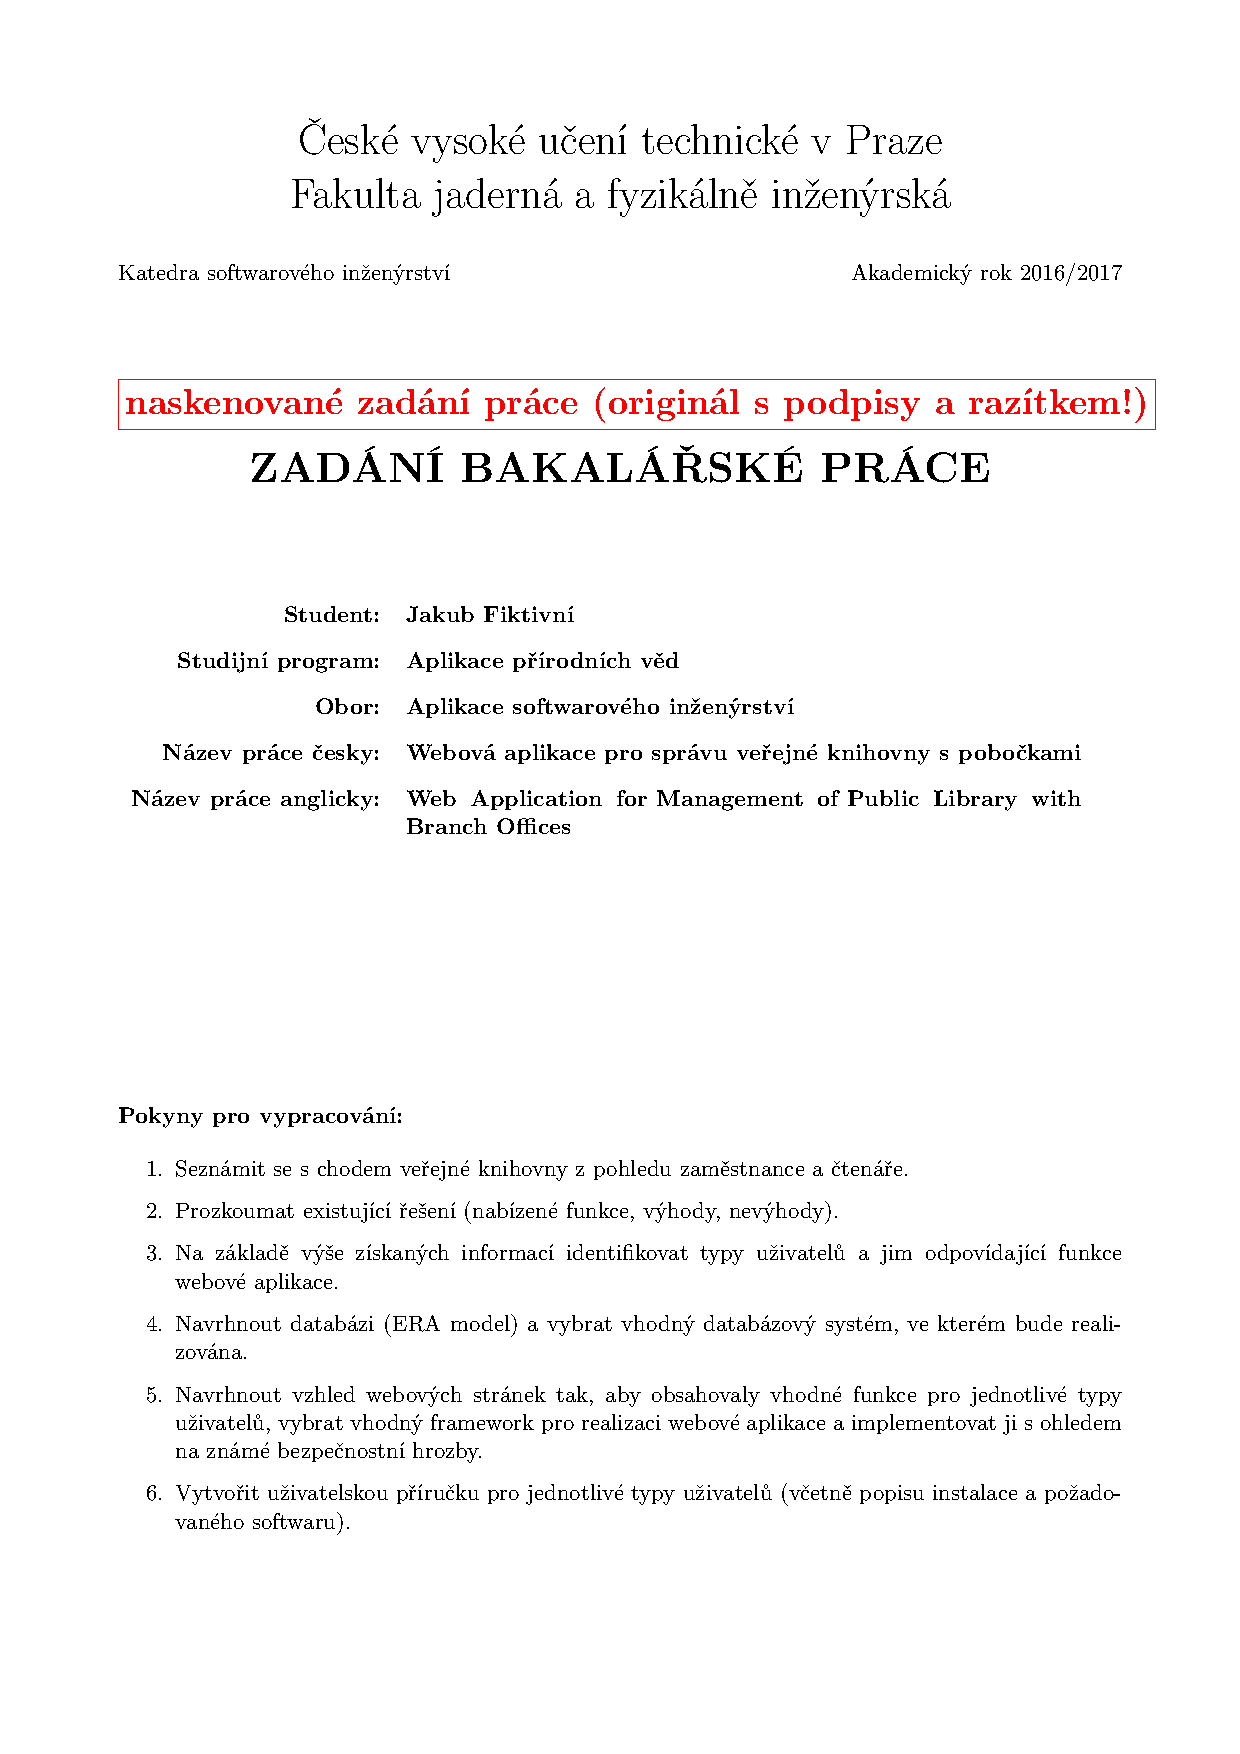
\includepdf[pages={1,2}]{resources/zadani_cele.pdf} % TODO: Replace with the correct paper




%%%%%%%%%%%% DECLARATION %%%%%%%%%%%%
\newpage 			  % DO NOT TOUCH!
\thispagestyle{empty} % DO NOT TOUCH!

~ 					  % DO NOT TOUCH!
\vfill 				  % Empty fill. DO NOT TOUCH!

\tb{Prohlášení} 	  % DO NOT TOUCH!

\vspace{1em} 		  % Vertical space. % DO NOT TOUCH!
\declarationCZ

\selectlanguage{american}%
\vspace{1em}
\tb{Declaration}

\vspace{1em}
\declarationEN
\selectlanguage{czech}%

\vspace{2em}  									 							  % DO NOT TOUCH!
\hspace{-0.5em}\begin{tabularx}{\textwidth}{X c} 							  % DO NOT TOUCH!
V \place\ dne .................... &........................................ \\ % DO NOT TOUCH!
	& \paperAuthor
\end{tabularx} % DO NOT TOUCH!




%%%%%%%%%%%% ACKNOWLEDGEMENT  %%%%%%%%%%%%
\newpage
\thispagestyle{empty}

~
\vfill % Empty fill

\tb{Poděkování}

\vspace{1em} % Vertical space. % DO NOT TOUCH!
\acknowledgementCZ

\selectlanguage{american}%
\vspace{1em}
\tb{Acknowledgment}

\selectlanguage{czech}%
\vspace{1em} % Vertical space. % DO NOT TOUCH!
\acknowledgementEN
\begin{flushright}
\paperAuthor
\end{flushright}  % Acknowledgement page ends here




%%%%%%%%%%%% ABSTRACT %%%%%%%%%%%% 
\newpage   			  % DO NOT TOUCH!
\thispagestyle{empty} % DO NOT TOUCH!

% Preparation: DO NOT TOUCH the next 8 lines!
\newbox\odstavecbox
\newlength\vyskaodstavce
\newcommand\odstavec[2]{%
    \setbox\odstavecbox=\hbox{%
         \parbox[t]{#1}{#2\vrule width 0pt depth 4pt}}%
    \global\vyskaodstavce=\dp\odstavecbox
    \box\odstavecbox}
\newcommand{\delka}{120mm} % Text width in 2nd table column

% Using the preparation: DO NOT TOUCH commands inside the "tabular" section!
\begin{tabular}{ll}
  {\em Název práce:} & ~ \\
  \multicolumn{2}{l}{\odstavec{\textwidth}{\bf \titleCZ}} \\[1em]
  {\em Autor:} & \paperAuthor \\[1em]
  {\em Studijní program:} & \programme \\
  {\em Obor:} & \specialization \\
  {\em Druh práce:} & \kind \\[1em]
  {\em Vedoucí práce:} & \odstavec{\delka}{\supervisor\\ \supervisorWorkspace} \\
  {\em Konzultant:} & -- %\odstavec{\delka}{\consultant \\ \consultantWorkspace}  % TODO: Remove the text "-- %" if you had a consultant
 \\[1em]  
  \multicolumn{2}{l}{\odstavec{\textwidth}{{\em Abstrakt:} ~ \abstractCZ  }} \\[1em]
  {\em Klíčová slova:} & \odstavec{\delka}{\keywordCZ} \\[2em]
  \selectlanguage{american}%
  {\em Title:} & ~\\
  \multicolumn{2}{l}{\odstavec{\textwidth}{\bf \titleEN}}\\[1em]
  {\em Author:} & \paperAuthor \\[1em]
  \multicolumn{2}{l}{\odstavec{\textwidth}{{\em Abstract:} ~ \abstractEN  }} \\[1em]
  {\em Key words:} & \odstavec{\delka}{\keywordEN}
\end{tabular}




%%%%%%%%%%%% CONTENTS OF THE PAPER %%%%%%%%%%%%
\selectlanguage{american}%
\newpage  		 % DO NOT TOUCH!
\parskip=0pt
\tableofcontents % DO NOT TOUCH!
\parskip=7pt
\newpage 		 % DO NOT TOUCH!




%--------------------------------------------------------
%|         The PAPER ITSELF begins here                 |
%--------------------------------------------------------

\chapter*{Introduction \TODO}		 		 % DO NOT TOUCH!
\addcontentsline{toc}{chapter}{Introduction \TODO} % DO NOT TOUCH!

Put my introduction text here (1-3 pages, do not divide it into sub-pages).

\chapter{Theory}
This chapter will present the core theory of areas used in this research assignment. Firstly, Graphical Processing Units (GPUs) will be introduced with an emphasis on the architecture of GPUs (only Nvidia GPUs as the Nvidia API, CUDA, was used to develop this project). Then, CUDA, will be described in greater detail. Finally, the theory behind Lower-Upper (LU) Decomposition will be presented.

\section{GPUs}
From an average consumer's perspective a Graphics Processing Unit (GPU) is a component of a computing system that performs graphical operations, for example, processing images. For the sake of the example, let image processing be simplified into the following: images are composed of pixels and each pixel needs to be processed. Since a GPU contains thousands of processing units it can perform a large number of operations in parallel, for example, processing a large number of pixels at once, thus making it highly efficient at image processing. While this has a wide range of uses, there is another field where the highly parallel nature of the GPU can be utilized: General-Purpose Computing on Graphics Processing Units (GPGPU).

\subsection{General-Purpose Computing on Graphics Processing Units (GPGPU)}
As described in Section~1.2 of the author's bachelor thesis \emph{Formats for storage of sparse matrices on GPU} \cite{Cejka2020}, GPUs started to evolve at the turn of the 21\textsuperscript{st} century from purely graphics-processing units into devices capable of general-purpose computing, i.e. computation that is not necessarily related to graphics. The significance of this event lies in the use of graphics cards for seemingly any parallelizable computational task that would benefit from the abundance of slower processing units on a GPU rather than fewer faster processing units found on a CPU \cite{NVIDIAMay2022}.

\par For reference, high-end desktop CPUs today usually have anywhere from 8 to 16 cores, while server CPUs can have upwards of 64 cores (not counting hyper-threading and similar technologies). In general, CPUs with more cores have a lower clock speed - see Figure~\ref{Figure:theory-GPUs-GPGPU-processor-comparison} for a selection of processors along with their core count and clock speeds \cite{Glawion7March2022}.

\begin{figure}[ht!]
	\centering
	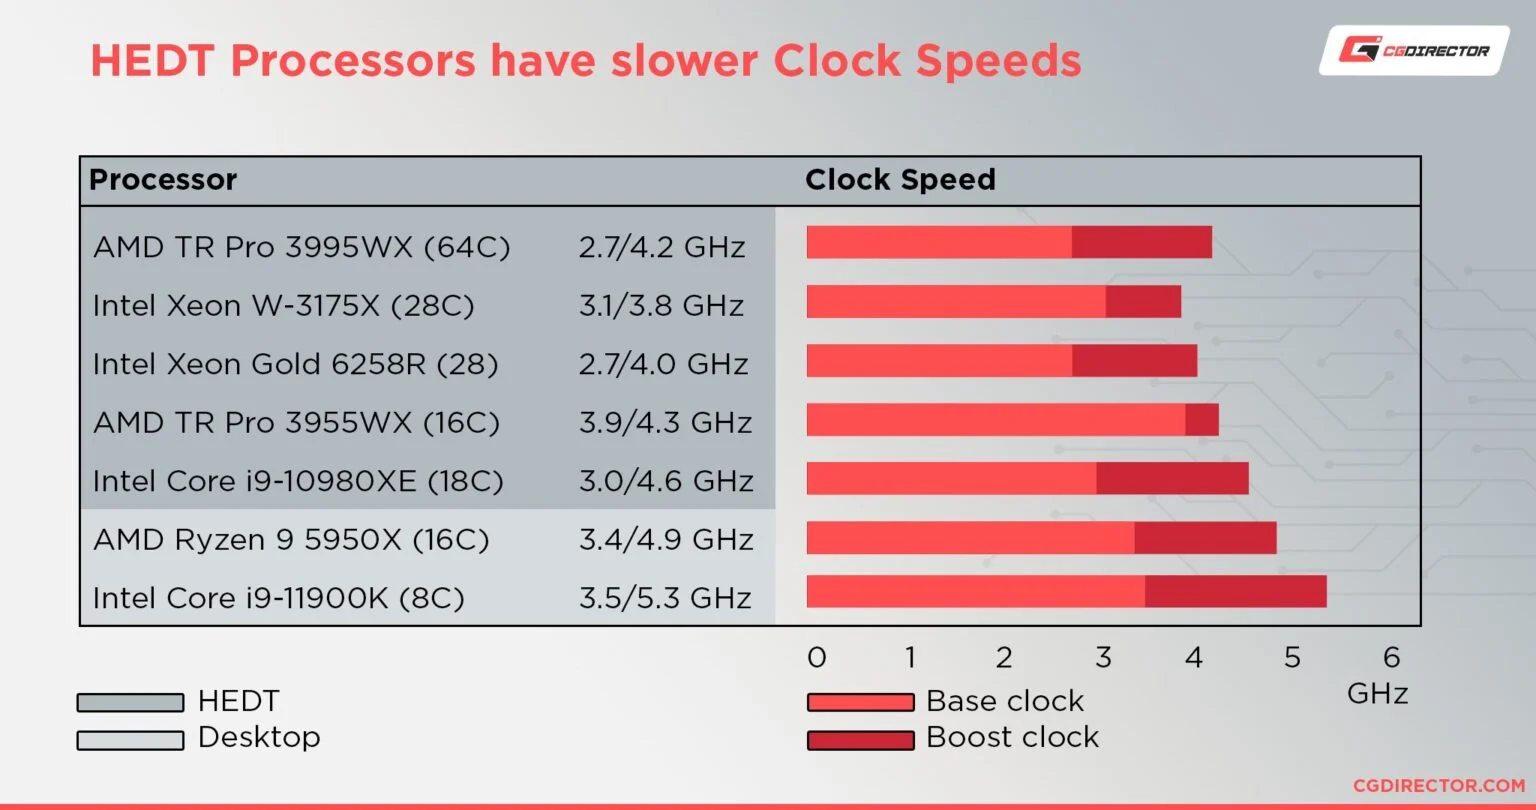
\includegraphics[width=14cm, keepaspectratio]{images/ch1/processors_comparison.png}
	\caption{Selection of desktop and server CPUs - including number of cores and clock speed \cite{Glawion7March2022}. HEDT stands for High-End Desktop Processor - in this instance it also includes CPUs predominantly used in servers.}
	\label{Figure:theory-GPUs-GPGPU-processor-comparison}
\end{figure}

While CPUs are widely used for sequential tasks, they can also be used for tasks that can be described as parallelizable, for example, processing of requests to a server. They are not suitable for highly parallel tasks such as image processing, where GPUs excel due to their architecture. Figure~\ref{Figure:theory-GPUs-GPGPU-nvidia-CPU-GPU-architecture-comparison} shows the comparison of a CPU and GPU architecture. The example CPU in the figure has - among other components - 4 cores each having its own L1 cache and controlling component. This configuration allows for executing a thread (series of operations) at a high speed and lower throughput (fewer number of threads running at once). Simply, the CPU is more suitable for rapid completion of serialized instructions.

\begin{figure}[ht!]
	\centering
	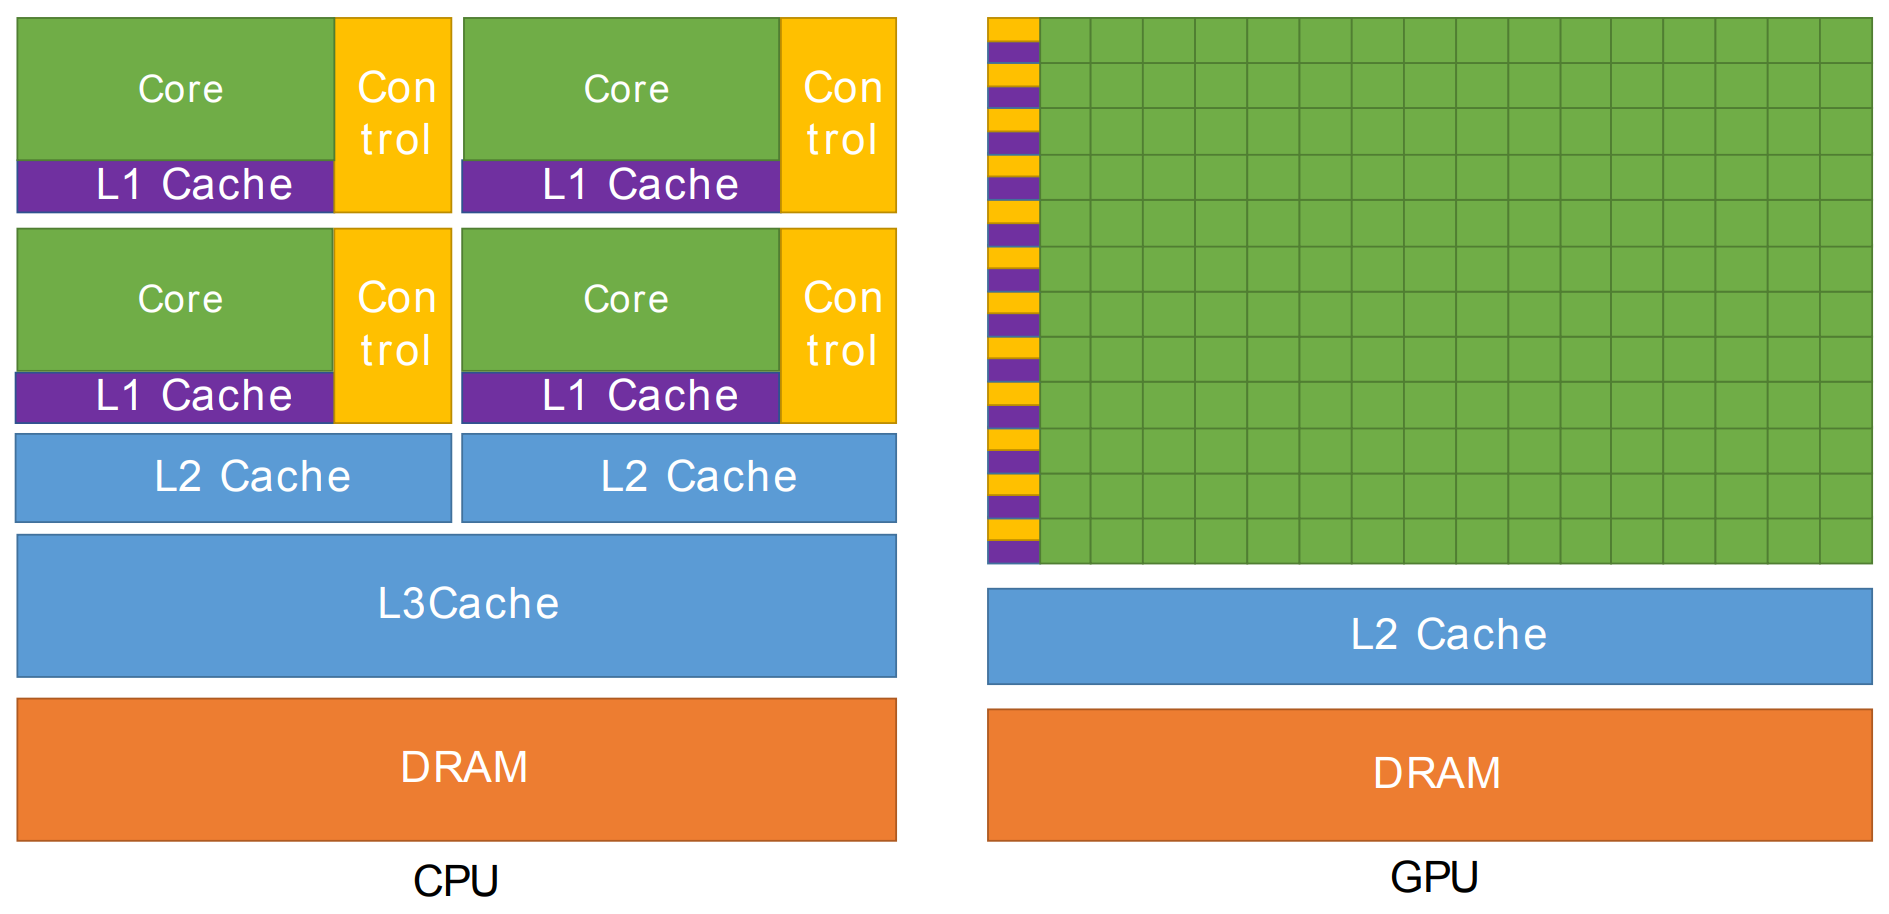
\includegraphics[width=14cm, keepaspectratio]{images/ch1/nvidia_CPU_GPU_comparison.png}
	\caption{Comparison of the architecture of CPUs and GPUs. On one hand, CPUs have fewer cores, more complex controlling logic compared to GPUs and the cores of a CPU have a higher clock speed. On the other hand, GPUs have a much higher number of cores clocked at lower speeds. Taken from Nvidia's \emph{CUDA C++ programming guide} \cite{NVIDIAMay2022}.}
	\label{Figure:theory-GPUs-GPGPU-nvidia-CPU-GPU-architecture-comparison}
\end{figure}

Nvidia GPUs, on the other hand, are engineered to have many smaller controlling units called SMs (Stream Multiprocessors) that aim to schedule and task individual processing units found on the GPU. Furthermore, in Figure~\ref{Figure:theory-GPUs-GPGPU-nvidia-CPU-GPU-architecture-comparison} it can be seen that GPUs have a different cache structure. Specifically, GPUs only have two levels, whereas CPUs have three. In summary, the GPU has more transistors for processing data - namely operations that use floating-point computations. Moreover, the architecture of the GPU allows for it to compensate for memory access delays by performing computations simultaneously \cite{NVIDIAMay2022}.
\par A prime example of where this characteristic gives a significant advantage to the GPU over the CPU is during matrix multiplication which will be described later in Section~\ref{Subsection:matrix-multiplication}.
\par For completion, see Table~\ref{Table:theory-GPUs-GPGPU-nvidia-gpu-details-comparison} for a selection of GPUs along with their specifications.

\begin{table}[ht!]
	\centering
	\renewcommand{\arraystretch}{0.9}
	\begin{tabular}{|>{\raggedright\arraybackslash\bfseries\scriptsize}m{2.7cm}|>{\scriptsize}m{2.7cm}|>{\scriptsize}m{2.7cm}|>{\scriptsize}m{2.7cm}|>{\scriptsize}m{2.7cm}|}
		\hline
		\rowcolor{nvidia}\multicolumn{1}{|>{\centering\arraybackslash\normalsize}m{2.72cm}|}{$\vcenter{\textbf{Nvidia}}$} 
		& \multicolumn{1}{>{\centering\arraybackslash\normalsize}m{2.72cm}|}{$\vcenter{\textbf{GTX 1070}}$}
		& \multicolumn{1}{>{\centering\arraybackslash\normalsize}m{2.72cm}|}{$\vcenter{\textbf{RTX 3060}}$}
		& \multicolumn{1}{>{\centering\arraybackslash\normalsize}m{2.72cm}|}{$\vcenter{\textbf{V100}}$}
		& \multicolumn{1}{>{\centering\arraybackslash\normalsize}m{2.72cm}|}{$\vcenter{\textbf{A100}}$}\\[5pt]
		\hline
		GPU & GP104 (Pascal) & GA106 (Ampere) & GV100 (Volta) & GA100 (Ampere) \\
		\hline
		\rowcolor{lightnvidia}\multicolumn{1}{|>{\arraybackslash\bfseries\scriptsize}m{2.72cm}|}{SMs}
		& \multicolumn{1}{>{\arraybackslash\scriptsize}m{2.72cm}|}{15}
		& \multicolumn{1}{>{\arraybackslash\scriptsize}m{2.72cm}|}{28}
		& \multicolumn{1}{>{\arraybackslash\scriptsize}m{2.72cm}|}{80}
		& \multicolumn{1}{>{\arraybackslash\scriptsize}m{2.72cm}|}{108} \\
		\hline
		TPCs & 15 & 14 & 40 & 54 \\
		\hline
		FP32 Cores / SM & NA &NA & 64 & 64 \\
		\hline
		FP32 Cores / GPU & NA & NA & 5,120 & 6,912 \\
		\hline
		FP64 Cores / SM & NA & NA & 32 & \\
		\hline
		FP64 Cores / GPU (excl. Tensor)	& NA & NA & 2,560 & 3,456 \\
		\hline
		CUDA Cores / SM & 128 & 128 & NA & NA \\
		\hline
		CUDA Cores / GPU & 1,920 & 3,584 & NA & NA \\
		\hline
		Tensor Cores / SM & NA & 4 & 8 & 16 \\
		\hline
		Tensor Cores / GPU & NA & 112 & 640 & 432 \\
		\hline
		GPU Boost Clock & 1683 MHz & 1777 MHz & 1530 MHz & 1410 MHz \\
		\hline
		\rowcolor{lightnvidia}\multicolumn{1}{|>{\arraybackslash\bfseries\scriptsize}m{2.72cm}|}{Peak FP32 TFLOPS}
		& \multicolumn{1}{>{\arraybackslash\scriptsize}m{2.72cm}|}{6.5}
		& \multicolumn{1}{>{\arraybackslash\scriptsize}m{2.72cm}|}{12.7}
		& \multicolumn{1}{>{\arraybackslash\scriptsize}m{2.72cm}|}{15.7}
		& \multicolumn{1}{>{\arraybackslash\scriptsize}m{2.72cm}|}{19.5}\\
		\hline
		\rowcolor{lightnvidia}\multicolumn{1}{|>{\arraybackslash\bfseries\scriptsize}m{2.72cm}|}{Peak FP64 TFLOPS}
		& \multicolumn{1}{>{\arraybackslash\scriptsize}m{2.72cm}|}{0.202}
		& \multicolumn{1}{>{\arraybackslash\scriptsize}m{2.72cm}|}{0.199}
		& \multicolumn{1}{>{\arraybackslash\scriptsize}m{2.72cm}|}{7.8}
		& \multicolumn{1}{>{\arraybackslash\scriptsize}m{2.72cm}|}{9.7}\\
		\hline
		Peak Tensor TFLOPS & NA & 51 & 125 & 312/624$^3$\\
		\hline
		\rowcolor{lightnvidia}\multicolumn{1}{|>{\arraybackslash\bfseries\scriptsize}m{2.72cm}|}{Memory Bandwidth}
		& \multicolumn{1}{>{\arraybackslash\scriptsize}m{2.72cm}|}{256 GB/s}
		& \multicolumn{1}{>{\arraybackslash\scriptsize}m{2.72cm}|}{360 GB/s}
		& \multicolumn{1}{>{\arraybackslash\scriptsize}m{2.72cm}|}{900 GB/s}
		& \multicolumn{1}{>{\arraybackslash\scriptsize}m{2.72cm}|}{1555 GB/s} \\
		\hline
		Texture Units & 120 & 112 & 320 & 432 \\
		\hline
		Memory Interface & 256-bit & 192-bit & 4096-bit HBM2 & 5120-bit HBM2 \\
		\hline
		Memory Size & 8 GB & 12 GB & 32 GB & 80 GB \\
		\hline
		L2 Cache Size & 2048 KB & 3072 KB & 6144 KB & 40960 KB \\
		\hline
		Shared Memory Size / SM & 96 KB & 128 KB & Configurable up to 96 KB & Configurable up to 164 KB \\
		\hline
		Register File Size / SM & 256 KB & 256 KB & 256 KB & 256 KB \\
		\hline
		Register File Size / GPU & 3840 KB & 7168 KB & 20480 KB & 27648 KB \\
		\hline
		\rowcolor{lightnvidia}\multicolumn{1}{|>{\arraybackslash\bfseries\scriptsize}m{2.72cm}|}{TDP}
		& \multicolumn{1}{>{\arraybackslash\scriptsize}m{2.72cm}|}{150 Watts}
		& \multicolumn{1}{>{\arraybackslash\scriptsize}m{2.72cm}|}{170 Watts}
		& \multicolumn{1}{>{\arraybackslash\scriptsize}m{2.72cm}|}{300 Watts}
		& \multicolumn{1}{>{\arraybackslash\scriptsize}m{2.72cm}|}{400 Watts}\\
		\hline
		Transistors & 7.1 billion & 12 billion & 21.1 billion & 54.2 billion \\
		\hline
		GPU Die Size & 314 mm$^2$ & 276 mm$^2$ & 815 mm$^2$ & 826 mm$^2$\\
		\hline
		Manufacturing Process & TSMC 16nm & Samsung 8N & 12 nm FFN & 7 nm N7\\
		\hline
	\end{tabular}
	\caption{Comparison of GPUs: GTX 1070 (Turing architecture), RTX 3060 (Ampere architecture), V100 (Volta architecture), A100 (Ampere architecture). The GPUs in this table assume the best possible configuration of their respective card, for example, the version with the most possible VRAM. Features that are important when it comes to card performance have been denoted in green. The data was obtained from various sources for the GTX 1070 \cite{Hagedoorn6October2016, oaUUFoT7oI5ApIyY, Smith18May2016, jAnwkq6mMKYTLUOB} the RTX 3060 \cite{Walton7July2021, wGXr33zSUweXiQMY, SMhyh0H3oh3nlda0, May1December2020}, the V100 \cite{NvidiaAugust2017} and the A100 \cite{soj8qSRbfefUdi8Y, rfiOEXAGDlcAOxF3}.}
	\label{Table:theory-GPUs-GPGPU-nvidia-gpu-details-comparison}
\end{table}

The table shows specifications for two different categories of GPUs: consumer and professional (commercial). Consumer cards (in the table: GTX 1070, RTX 3060) can be found in regular desktop PCs and are intended more for video gaming, rather than raw computing power. However, these cards are mentioned as the optimization of this project's implementation was done on machines that included them. On the other hand, professional cards are intended mainly for GPGPU, or - in some specific cases - for machine learning. \\
Characteristics that can be used to compare GPUs are, for example, peak TFLOPS (TFLOPS - how many trillion floating-point operations can the processor perform per second), memory bandwidth, TDP. The value that clearly separates commercial cards from consumer cards is the peak FP64 (double precision) TFLOPS, which is the highest for the A100 at 9.7 TFLOPS, with the V100 being slightly slower at 7.8 TFLOPS, whereas the consumer cards perform significantly worse at around 0.2 TFLOPS. \\
In summary, professional cards are heavily preferred when it comes to GPGPU, however, consumer cards can be and are used for development as they are more affordable.



\section{Compute Unified Device Architecture (CUDA)}\label{Section:theory-CUDA}
The Compute Unified Device Architecture (CUDA) is programming model, sometimes referred to as a parallel computing platform, introduced by Nvidia in 2006 \cite{Oh10September2012}. It is designed to give developers low-level access to GPU hardware, for example, fine-tuning assignment of processing units or memory allocation, thus, allowing them to utilize the full potential of GPUs and tailor their use for specific applications. CUDA supports a variety of programming languages, for example, C++ (used in this project) and Fortran, however, adaptations for other languages such as, Python, Perl, Java, Ruby, MATLAB, Julia, etc. have been created \cite{OsGyRFLMngy0j8Pv}.
\par This section will first explain some basic terminology followed by the theory behind CUDA from the simplest concept - a thread - to how threads are managed. Then, memory will be introduced in a similar manner: from per-thread local memory to global memory. Subsequently, asynchronous concurrent execution will be described. Finally, basic CUDA extensions of the C++ language will be presented and their translation into the thread and memory management systems will be shown on a simple example program.

\subsection{Introductory Terminology}\label{Subsection:theory-CUDA-introductory-terminology}
CUDA introduces many unique concepts that come with their own naming scheme. This section will list and explain some basic terminology that will be used throughout the project \cite{Ruetsch2008}:
\begin{itemize}
	\item \textbf{Host} - Central Processing Unit (CPU) and its memory. The host provides data to GPU and instructs it to execute various instructions.
	\item \textbf{Device} - Graphics Processing Unit (GPU) and its memory. The device executes specialized instructions provided by the host.
	\item \textbf{Kernel} - term used for a special type of function that, unlike regular functions, can only be called from the host and executed on the device. Furthermore, when a CUDA kernel is called it is executed in parallel across a number of threads.	
\end{itemize}

\subsection{Thread Management}\label{Subsection:thread-management}
This section will aim to describe how CUDA handles its basic execution units: threads. First, a thread itself will be defined and described followed by explanations of multiple encompassing thread structures.

\paragraph{CUDA thread}
The thread management system within CUDA begins, at the most basic level, with its smallest execution unit, a thread. According to \emph{CUDA C++ Programming Guide} a thread is an executed sequence of operations \cite{NVIDIAMay2022}. Due to the highly parallel nature of the GPU - spreading the workload across thousands of execution units - a CUDA thread is designed to be lightweight (unlike a typical CPU thread - assuming no hyper-threading is present). In this context, 'lightweight' signifies that the GPU is capable of easily switching between threads. An example showing how a set of instructions can be run on a set of 8 threads can be seen in Figure~\ref{Figure:theory-CUDA-thread-parallelism}. \\
In this project, the terms 'CUDA thread' and 'thread' will be used interchangeably. For a more detailed explanation of the difference between a CUDA thread and that of the CPU see \emph{Formats for storage of sparse matrices on GPU} \cite{Cejka2020}.

\begin{figure}[ht!]
	\centering
	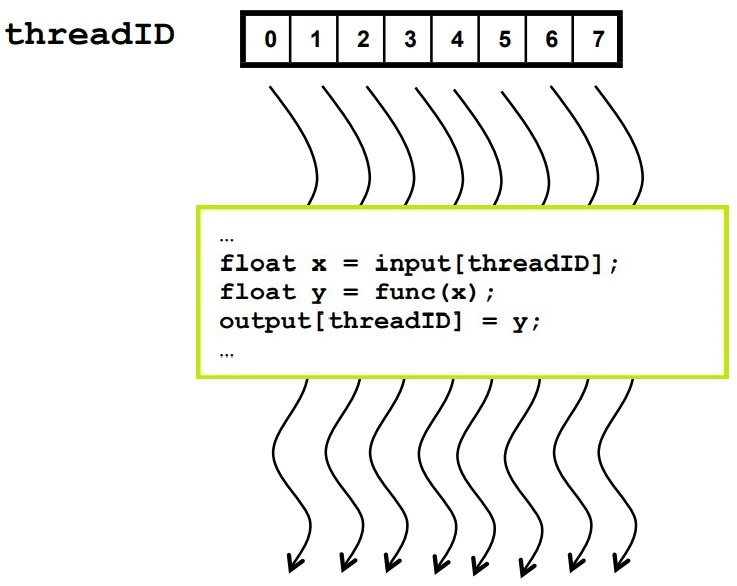
\includegraphics[width=9.5cm, keepaspectratio, clip]{images/ch1/CUDA_thread_parallelism.jpg}
	\caption{On an Nvidia GPU, eight threads with IDs from \code{0} to \code{7} execute the code in this example. A value from the array \code{input} with \code{threadID} as the index (i.e. each thread will read a value at a different index) is changed using the function \code{func(x)} and then stored in the same order as before into the array \code{output}. Taken from \emph{Format for storage of sparse matrices on GPU} \cite{Cejka2020, Ruetsch2008}.}
	\label{Figure:theory-CUDA-thread-parallelism}
\end{figure}

\paragraph{Warp}\label{Paragraph:theory-CUDA-thread-management-warp}
To execute thousands of threads simultaneously, SMs of an Nvidia GPU use the Single-Instruction Multiple-Thread (SIMT) execution model. The abbreviation SIMT comes from the amalgamation of SIMD (Single-Instruction Multiple-Data) and multi-threading (executing multiple sequences of instructions simultaneously). Specifically, this approach comprises of multiple threads executing the same computations on different data items \cite{Marziale2010}. In terms of CUDA, the core of the SIMT architecture is a so-called 'warp' that is made up of 32 threads. In other words, the smallest number of threads that can be executed simultaneously is 32. If fewer threads are required, for example, only one thread, then CUDA will still allocate 32 threads with 31 being inactive. Similarly, if a subset of threads from a warp are to execute different instructions (e.g., as a result of a conditional statement) then the different sets of instructions are executed serially across their respective threads - this issue is known as 'thread divergence'. An example of thread divergence can be seen in Figure~\ref{Figure:theory-CUDA-warp-thread-divergence}; the warp in the example is simplified for the purpose of the explanation and as such contains only 8 threads.

\begin{figure}[ht!]
	\centering
	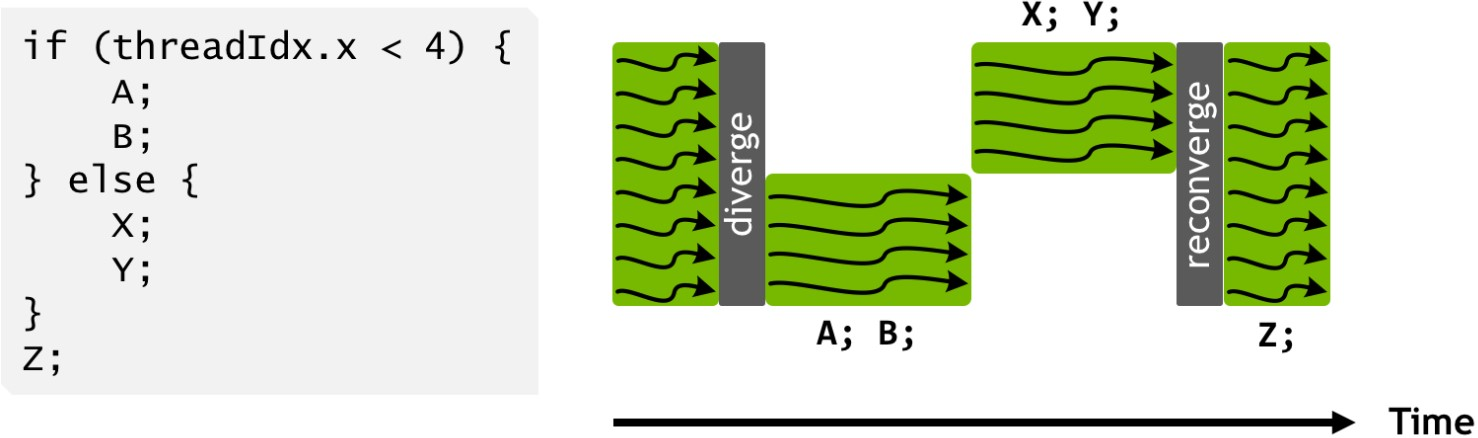
\includegraphics[width=14cm, keepaspectratio]{images/ch1/CUDA_warp_divergence_execution_path.jpg}
	\caption{Conditional code execution by a warp of 8 threads; each thread is represented by one wavy line. Due to the condition, threads with an ID between \code{0} and \code{3} will only execute statements \code{A} and \code{B}. However, simultaneously, threads with IDs between \code{4} and \code{7} will be put on hold. Comparably, while threads with IDs between \code{4} and \code{7} will be executing statements \code{X} and \code{Y}, the remaining threads will be idle. Thus, thread divergence has occurred within the 8-thread warp. Taken from Nvidia's developer blog post: \emph{Inside Volta: The World's Most Advanced Data Center GPU} \cite{Durant10May2017}.}
	\label{Figure:theory-CUDA-warp-thread-divergence}
\end{figure}

\paragraph{Block}\label{Paragraph:theory-CUDA-thread-management-block}
It is not always necessary to use such granularity that warps are able to provide. Developers can choose to execute code on a group of up to 1024 threads (with CUDA Compute Capability greater than 3.5) - referred to as a block. Threads in a block can cooperate via shared memory (subsection \ref{Subsection:memory-management} will explain more) and they can be synchronized - this is not possible for threads in different blocks. Threads in a block can be structured in 1, 2, or 3 dimensions (x, y, z); each thread has a unique ID in every dimension. The 1024 threads-per-block limit encompasses all 3 possible dimensions, in other words, the total number of threads must be at most 1024 across all dimensions (\code{num\_threads\_x\_dim} $ \cdot $ \code{num\_threads\_y\_dim} $ \cdot $ \code{num\_threads\_z\_dim} $ \leq$ 1024) \cite{AbiChahla18June2008, NVIDIAMay2022}.

\paragraph{Grid}\label{Paragraph:theory-CUDA-thread-management-grid}
In terms of CUDA a grid consists of multiple blocks of threads. Similarly to how threads can be structured within blocks, blocks can be structured within grids - up to 3 dimensions of blocks; each block has a unique ID in every dimension. The maximum number of blocks in every dimension is set to $ 2^{31} - 1 $ (65 536). One of the main reasons for having another structure on top of blocks (apart from memory management - detailed explanation in Section~\ref{Subsection:memory-management}) stems from the fact that while the limit for threads per block is set to 1024, GPUs are capable of running a multitude more threads in parallel. This means that the grid structure allows for the same code to be executed simultaneously on a group of thread blocks. However, it is important to note that there is a limit of how many threads can be active at once. When this limit is reached, blocks of threads are executed sequentially in such a way that allows for near-maximal concurrently active threads. Another noteworthy aspect is the difference between the terms 'number of allocated threads' and 'number of active threads'. The former means how many threads are allocated in total, i.e. both active (currently executing) and inactive (scheduled) threads, whereas the latter refers to threads that are actively being executed at a point in time. \\
A visualization of CUDA's thread structuring can be seen in Figure~\ref{Figure:theory-CUDA-grid-block-thread}.

\begin{figure}[ht!]
	\centering
	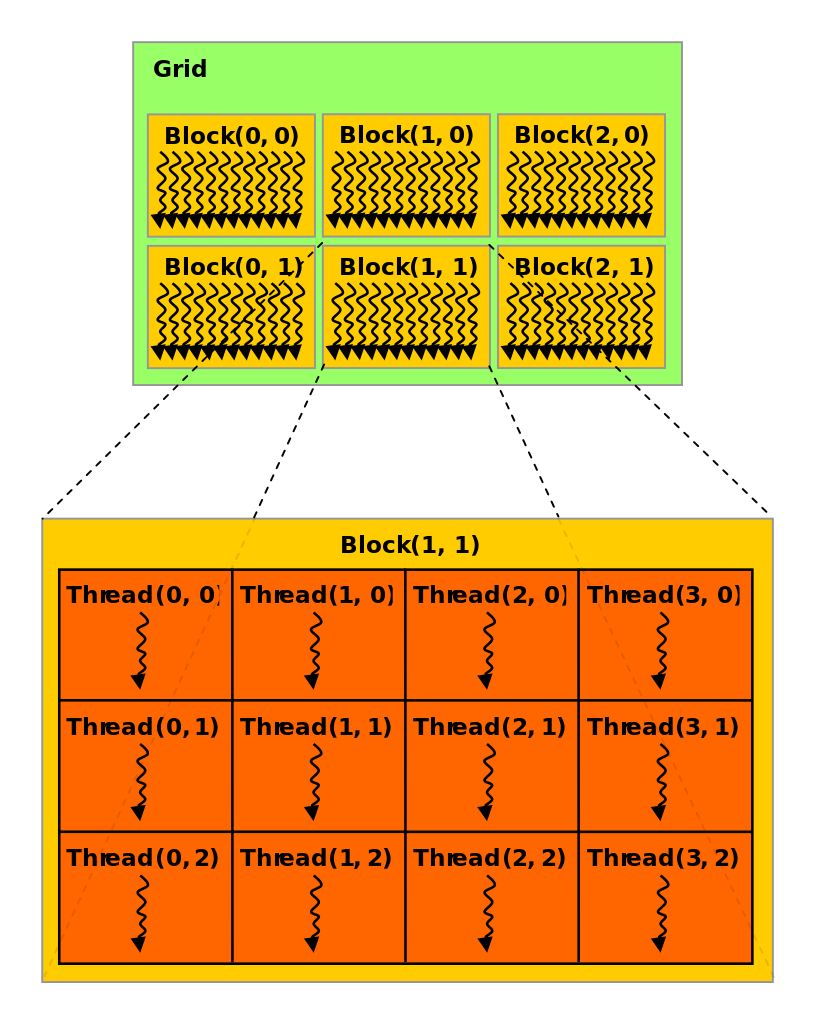
\includegraphics[width=11cm, keepaspectratio]{images/ch1/nvidia_grid_block_thread.png}
	\caption{CUDA thread structuring of a 2D grid made up of 2D blocks of threads. Taken from Nvidia's \emph{CUDA C++ Programming Guide} \cite{NVIDIAMay2022}.}
	\label{Figure:theory-CUDA-grid-block-thread}
\end{figure}


\subsection{Memory Management}\label{Subsection:memory-management}
The aim of this section is to present how memory management works in CUDA. Different types of memory available on the GPU will be presented, ranging from per-thread local to global memory.

\paragraph{Per-thread local memory}
When a kernel is executed on the GPU across a number of threads every thread has its own unique ID stored in a variable that is available within the kernel. This variable is stored in memory that is referred to as \textit{per-thread local memory}. In other words, every thread has its own local memory where it can store variables. It is important to note that per-thread local memory consists of two different types - registers and local memory. Registers is on-chip memory (low latency and high bandwidth), however, it is limited in capacity at 255 32-bit registers per thread in CUDA Compute Capability 3.5 and higher, which does not allow for extensive kernels containing many variables. The compiler will store almost all variables allocated within the kernel into registers, with the exception of \cite{NVIDIAMay2022}:
\begin{itemize}
	\item Arrays indexed with constant quantities
	\item Large structures or arrays that would use too much registers space
	\item Any variable if the kernel uses more registers than available - called \textit{register spilling}
\end{itemize}
The variables and structures mentioned above that the compiler will not store in registers will instead be stored in purely local memory which resides in device memory. Device memory is also referred to as global memory which is off-chip and therefore, any accesses by threads into their purely local memory will be slower than accessing registers. Figure~\ref{Figure:theory-CUDA-memory-types-detailed} shows available accesses of threads to different types of memory. \\
As of CUDA Compute Capability 3.5, the amount of purely local memory available for every thread is only 512 KB \cite{NVIDIAMay2022}. In summary, per-thread local memory is often used sparingly to avoid register spilling and the accompanied slower memory access, however, if used efficiently, it can be helpful when complex indexing is required for some calculations.

\paragraph{Shared memory}\label{Paragraph:theory-CUDA-memory-management-shared-memory}
The next layer of memory is per-block memory referred to as \textit{shared memory}. As the name suggests, this memory is shared by all threads belonging to a particular block. Similarly to registers, shared memory is on-chip and therefore it is fast, however, it is also limited in capacity depending on the CUDA Compute Capability version - see table \ref{Table:theory-CUDA-block-max-shared-memory} for specific values.

\begin{table}[ht!]
	\centering
	\renewcommand{\arraystretch}{1.5}
	\begin{tabular}{ |c|c|c|c|c|c|c| } 
		\hline
		Compute Capability & 3.5 - 6.2 & 7.0 - 7.2 & 7.5 & 8.0 & 8.6 & 8.7 \\
		\hline
		Max. shared memory per block [KB] & 48 & 96 & 64 & 163 & 99 & 163 \\
		\hline
	\end{tabular}
	\caption{Maximum shared memory per thread block across different CUDA Compute Capabilities. Nvidia notes in their documentation that any value above 48 KB requires the use of dynamic shared memory. Taken from Nvidia's \emph{CUDA C++ Programming Guide} \cite{NVIDIAMay2022}.}
	\label{Table:theory-CUDA-block-max-shared-memory}
\end{table}

Shared memory can either be allocated statically or dynamically. The former needs the size of allotted memory to be known at compile time, for example, an array of constant size denoted within the kernel using a dedicated prefix that indicates it is meant to be stored in the shared memory of each thread's block. On the other hand, the latter - dynamic allocation of shared memory - allows for the size of required memory to be determined at runtime, however, this means that the developer must specify the size of the shared memory as one of the parameters when calling the kernel.

\begin{figure}[ht!]
	\centering
	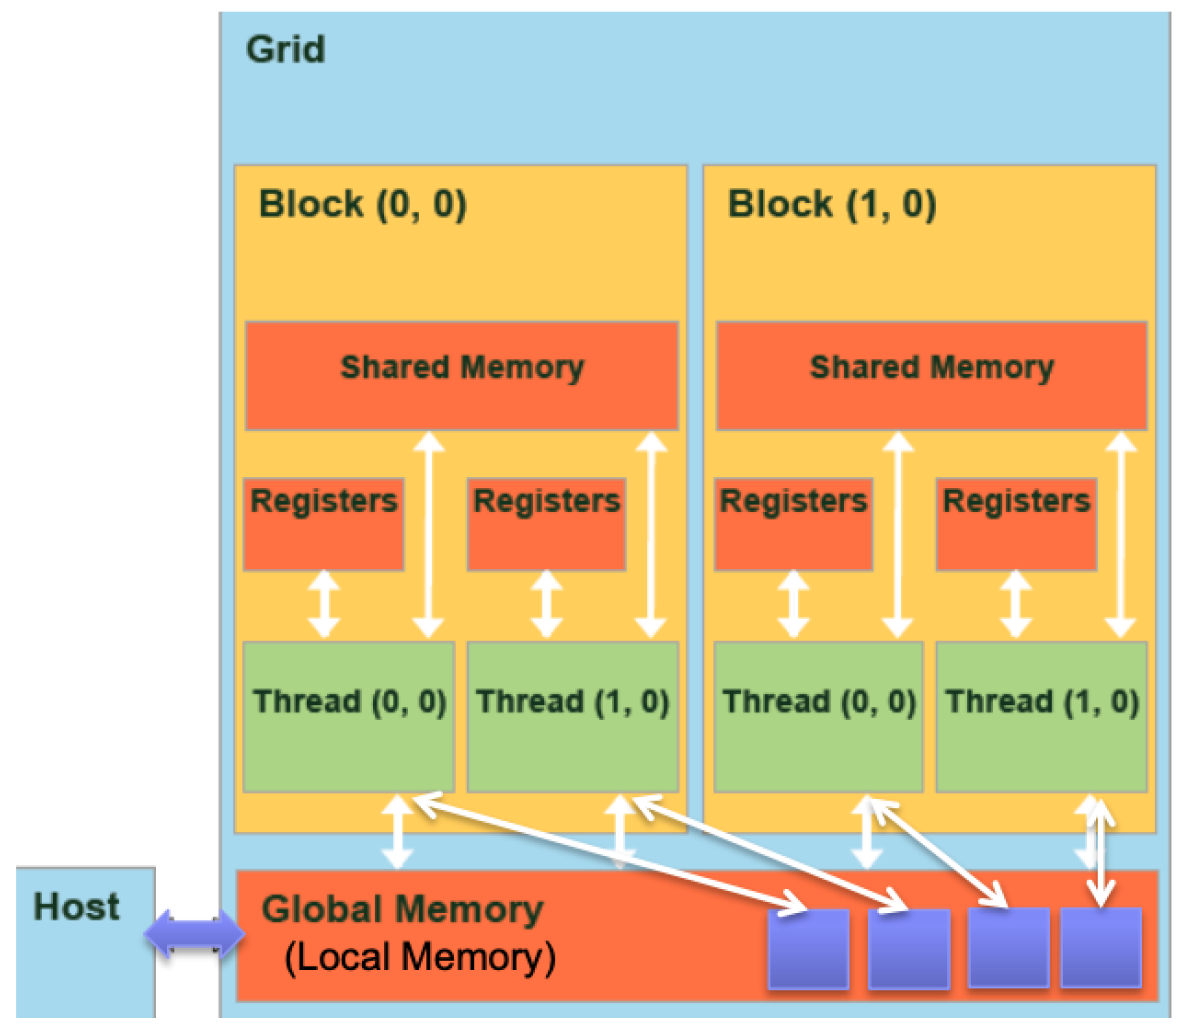
\includegraphics[width=11cm, keepaspectratio]{images/ch1/CUDA_memory_types_detailed.png}
	\caption{Different CUDA memory types visualized. Each thread has access to its local memory comprised of registers, local memory (blue squares in global memory), shared memory of its block, and global memory. Taken from Yao Hsiao's \emph{GPU - CUDA introduction} \cite{Hsiao17December2019}.}
	\label{Figure:theory-CUDA-memory-types-detailed}
\end{figure}

Shared memory of each block is divided into 32-bit (4-byte) memory modules called words. A single word can store a float, half a double, 32-bit int, etc. - anything that can be stored in 32 bits. Apart from words, there are 32 banks per block. Each bank contains a number of words depending on the size of shared memory allocated. Since the size of shared memory can be up to 48 KB or more - depending on the version of CUDA Compute Capability - then the number of words per bank can differ between versions. Figure~\ref{Figure:theory-CUDA-shared-memory-banks-words} visualizes the division of shared memory into banks and words.

\begin{figure}[ht!]
	\centering
	\begin{subfigure}{\textwidth}
		\centering
		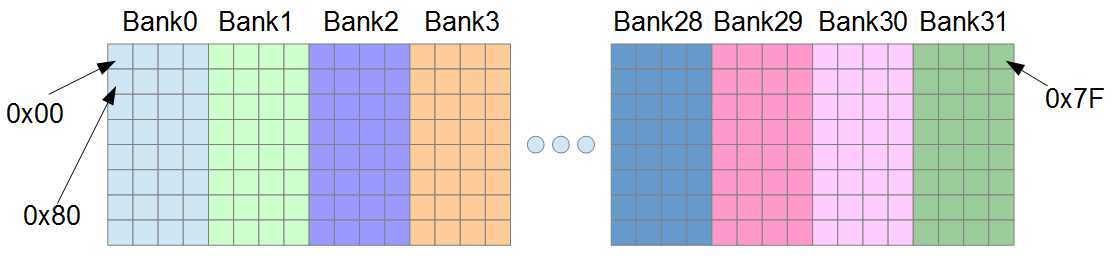
\includegraphics[width=14.5cm, keepaspectratio]{images/ch1/CUDA_shared_memory_banks_words.png}
		\subcaption{Shared memory divided into banks (columns under each \code{Bank*}), words (4 same-color squares of a row) and bytes (individual squares). In the first row, the first 4 bytes under \code{Bank0} - beginning at address \code{0x00} - make up the \code{0th} word (as show in Figure). The four bytes to the right of it (first row under \code{Bank1}) make up the \code{1st} word. Memory addresses of some bytes are shown hexadecimal.}
		\label{Figure:theory-CUDA-shared-memory-banks-words-bytes}
	\end{subfigure}

	\begin{subfigure}{\textwidth}
		\centering
		\hspace*{-0.8cm}
		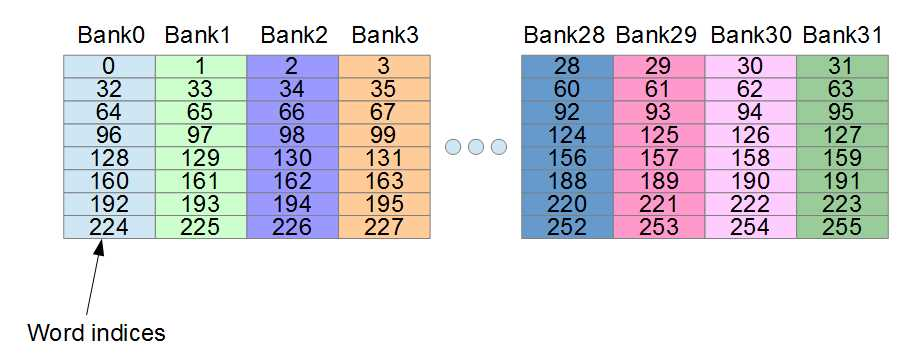
\includegraphics[width=13cm, keepaspectratio]{images/ch1/CUDA_shared_memory_banks_words_indices.png}
		\subcaption{Shared memory divided into banks (column under each \code{Bank*}) and words (individual rectangles with IDs inside).}
		\label{Figure:theory-CUDA-shared-memory-banks-words-ids}
	\end{subfigure}
	\caption{Illustration of shared memory. In this example, there are 32 banks; each one has eight 4-byte (32-bit) words - in Figure~\ref{Figure:theory-CUDA-shared-memory-banks-words-bytes} one byte is one square. Reading and writing into the \code{0th}, \code{32nd}, \code{64th}, etc. word is the responsibility of \code{Bank0}; reading and writing into the \code{1st}, \code{33rd}, \code{65th}, etc. word is the responsibility of \code{Bank1} and so on. Taken from \emph{Chapter 6: Shared Memory} of \emph{Cuda Succinctly} \cite{Rose2017}.}
	\label{Figure:theory-CUDA-shared-memory-banks-words}
\end{figure}

Manipulating memory in banks can be fast and efficient under certain conditions. Let us consider the following example: Figure~\ref{Figure:theory-CUDA-shared-memory-banks-words-ids} is the shared memory of a block that is used in a kernel. In this kernel, there is an array made up of 256 floats (32-bit) - each word in the figure is a single float. Furthermore, the IDs of words in the figure correspond to indices of floats in the array, thus, float values stored next to each other in memory belong to successive banks, for example, \code{arr[0]} belongs to \code{Bank0}, \code{arr[1]} belongs to \code{Bank1}, \code{arr[32]} belongs to \code{Bank0}, etc. \\
As mentioned by Chris Rose in \emph{CUDA Succinctly} \cite{Rose2017}, this division of words into banks is salient as each bank can serve only one word to a warp at once. This means that if a single word is requested from each bank, then all 32 threads of a warp can be served by all 32 banks simultaneously and expeditiously. Data serving is also fast when the same word from shared memory is accessed by all threads of a warp; this is called a \textit{broadcast} as shared memory is read once and the value is sent to all threads of the warp at once. \\
A concept similar to broadcasting is called a \textit{multicast}, which is an operation that is used when the same word from any particular bank is accessed by more than one thread of a warp. In this case, the threads that accessed the word will all receive it simultaneously from its bank. Under good conditions, the multicast operation is as fast as a broadcast. It is important to note that multicast is only available for compute capability 2.0 and higher. \\
However, the operations above all assumed good conditions for reading and writing of data. The primary originator of bad conditions for accessing shared memory is called a \textit{bank conflict}. Bank conflict describes an instance when threads of a warp request more than one word from any single bank. When this occurs, reading and writing of a word will be performed serially by the bank. For example - looking at Figure ~\ref{Figure:theory-CUDA-shared-memory-banks-words-ids} - let thread \code{0} and thread \code{1} access words \code{0} and \code{32} respectively. Since both words belong to \code{Bank0}, then a bank conflict has occurred and the bank cannot distribute words' data in parallel. Instead, \code{Bank0} will firstly serve thread \code{0} with word \code{0} and then thread \code{1} with word \code{32}. \\
In order to facilitate further understanding, examples from \emph{Cuda succinctly} \cite{Rose2017} and \emph{CUDA C++ Programming Guide} \cite{NVIDIAMay2022} are included below. \\
Firstly, Table~\ref{Table:theory-CUDA-shared-memory-access-patterns} presents different shared memory access patterns - including notes on the speed of execution. Then, Figure~\ref{Figure:theory-CUDA-shared-memory-banks-words-no-conflicts} portrays shared memory access using random permutations, multicast and broadcast. Finally, Figure~\ref{Figure:theory-CUDA-shared-memory-banks-words-conflicts} shows examples of strided shared memory access with and without bank conflict - additionally, this figure also visualizes some examples from Table~\ref{Table:theory-CUDA-shared-memory-access-patterns}.

\begin{table}[ht!]
	\centering
	\renewcommand{\arraystretch}{1.5}
	\begin{tabular}{ |l|l| } 
		\hline
		\textbf{Access Pattern} & \textbf{Notes} \\
		\hline
		\code{arr[0]}			& Fast - broadcast to all threads of the grid \\
		\hline
		\code{arr[bID]}			& Fast - broadcast to all threads of a block \\
		\hline
		\code{arr[tID]} 		& Fast - all threads request from different banks \\
		\hline
		\code{arr[tID/2]} 		& Fast - multicast; every two threads read from the same bank \\
		\hline
		\code{arr[tID*2]} 		& Slow - two-way bank conflict \\
		\hline
		\code{arr[tID*3]} 		& Fast - all threads access different banks \\
		\hline
		\code{arr[tID*32]} 		& Egregiously slow - 32-way bank conflict \\
		\hline
	\end{tabular}
	\caption{Access patterns to shared memory. \code{arr} is an array stored in the shared memory of a thread block. \code{tID} is the ID of a thread and \code{bID} is the ID of a block. Taken from \emph{Chapter 6: Shared Memory} of \emph{Cuda Succinctly} \cite{Rose2017}.}
	\label{Table:theory-CUDA-shared-memory-access-patterns}
\end{table}

\begin{figure}[ht!]
	\centering
	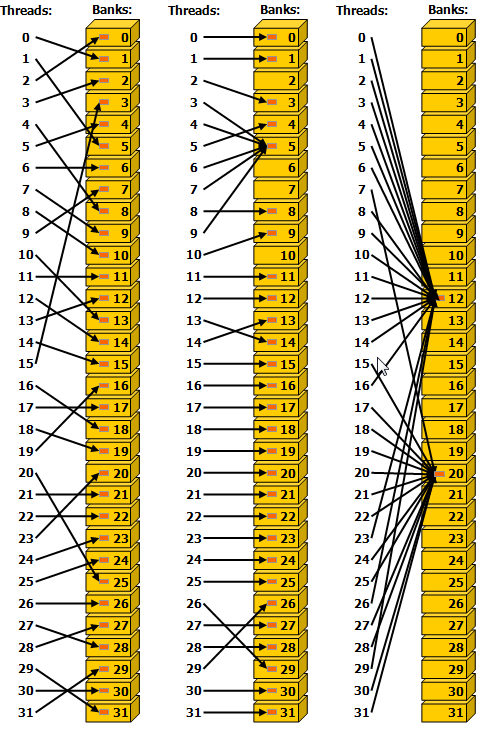
\includegraphics[width=11cm, keepaspectratio]{images/ch1/CUDA_shared_memory_banks_words_no_conflicts.png}
	\caption{Irregular shared memory accesses on 3 separate examples; yellow rectangular cuboids are banks; small orange rectangles are words. The left sub-image shows threads of a warp accessing shared memory randomly, however, in such a way that does not cause bank conflicts. The middle sub-image shows shared memory accessed by threads using the multicast operation, specifically, threads 3, 4, 5, 6, 7 and 9 accessing the same word from bank 5; other threads all access one word any bank each - no bank conflict. The right sub-image shows threads accessing shared memory via two broadcast operations. Taken from Nvidia's \emph{CUDA C++ Programming Guide} \cite{NVIDIAMay2022}.}
	\label{Figure:theory-CUDA-shared-memory-banks-words-no-conflicts}
\end{figure}

\begin{figure}[ht!]
	\centering
	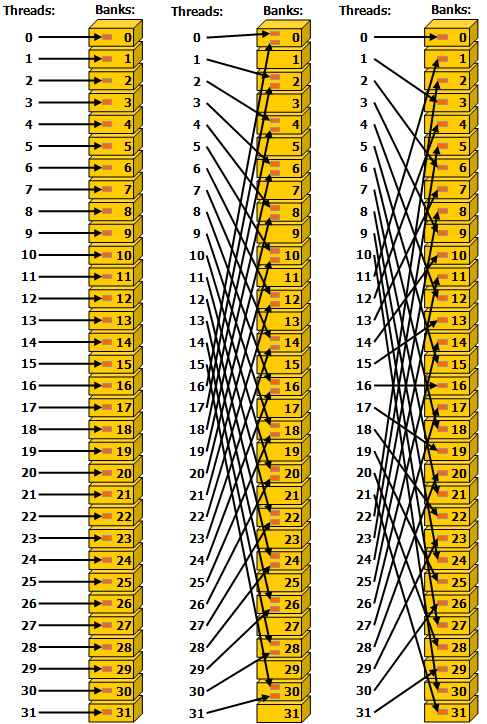
\includegraphics[width=11cm, keepaspectratio]{images/ch1/CUDA_shared_memory_banks_words_conflicts.png}
	\caption{Shared memory access using striding on 3 separate examples; yellow rectangular cuboids are banks; small orange rectangles are words. The left sub-image shows threads of a warp accessing shared memory with a stride of 1 (no bank conflict). The middle sub-image shows shared memory accessed by threads with a stride of 2 (equivalent to \code{arr[tID*2]} from Table~\ref{Table:theory-CUDA-shared-memory-access-patterns}; two-way bank conflict as threads access two different words from the same bank). The right sub-image shows threads accessing shared memory with a stride of 3 (equivalent to \code{arr[tID*3]} from Table~\ref{Table:theory-CUDA-shared-memory-access-patterns}; no bank conflict). Taken from Nvidia's \emph{CUDA C++ Programming Guide} \cite{NVIDIAMay2022}.}
	\label{Figure:theory-CUDA-shared-memory-banks-words-conflicts}
\end{figure}

In summary, ensuring that bank conflicts do not occur is pivotal to achieving efficient use of shared memory and subsequently high bandwidth.

\paragraph{Global memory}\label{Paragraph:theory-CUDA-memory-management-global-memory}
The final, all-accessible memory layer is called \textit{global memory}. Some sources also refer to it as \textit{device memory} since global memory resides in the device's DRAM (Dynamic Random Access Memory) - not to be confused with the host's memory, often referred to as, RAM. The modifier 'global' represents the all-accessible aspect of this type of memory, as it can be accessed by the host and the device, thus, serving as a memory communication medium that can be used to transfer data between the two, and house input and output data for kernels \cite{Harris7January2013}. Global memory is available for all threads on the device, regardless of what thread structure they belong to. In other words, all grids have access to the same global memory - shown in Figure~\ref{Figure:theory-CUDA-memory-management}.

\begin{figure}[ht!]
	\centering
	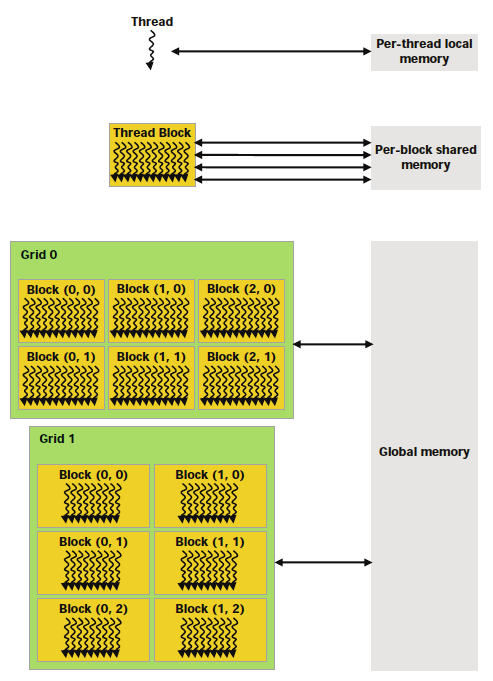
\includegraphics[width=11cm, keepaspectratio]{images/ch1/CUDA_memory_management.png}
	\caption{CUDA memory structuring. Taken from Nvidia's \emph{CUDA C++ Programming Guide} \cite{NVIDIAMay2022}.}
	\label{Figure:theory-CUDA-memory-management}
\end{figure}

Unlike shared memory, global memory functions similarly to RAM: it is initialized with the startup of the program, it will be available while the program is running, and it is terminated with the termination of the program. In order to use global memory, the developer must manually allocate memory on the device, then copy the data from the host to the device, and finally, deallocate (free) the data from the device \cite{Harris7January2013} once it is not required. \\
As mentioned above, in Paragraph~\emph{Per-thread local memory} in Section~\ref{Subsection:memory-management}, for the purpose of this project global memory is assumed to be off-chip - for completion, an exception to this is mentioned by Mark Harris in \emph{How to Access Global Memory Efficiently in CUDA C/C++ Kernels} \cite{Harris7January2013}: "\textit{Depending on the compute capability of the device, global memory may or may not be cached on the chip.}". Accessing (reading and writing) global memory is slower than accessing the aforementioned types of memory. In order to minimize this bottleneck, it is advised by Nvidia to keep the number of transactions that require accessing global memory to as few as possible \cite{Harris7January2013}. One of the main concepts that achieves this is called \textit{global memory coalesced access}. This methodology takes full advantage of the SIMD approach, specifically, instruction execution by threads in warps. In other words, it uses the fact that threads in a warp execute the same instruction simultaneously - in this instance: combine multiple memory accesses into a single transaction. \\
This means that upon the execution of a load instruction by all threads in a warp, the device will detect whether the threads are attempting to access successive global memory locations. If the accessed addresses are successive, then the accesses are coalesced (amalgamated) by the device into a consolidated access to consecutive DRAM locations \cite{Cabrera4December2019}. \\
More specifically, a single coalesced access into global memory - composed of a single access instruction performed by threads of a warp - occurs only if the following conditions are satisfied \cite{xUOrKLpxlGjvTonr, NVIDIAMay2022}:

\begin{enumerate}\label{Enumerate:theory-CUDA-global-memory-coalesced-access-requirements}
	\item Each thread accesses a memory element of size 4, 8, or 16 bytes
	\item The device memory is accessed by memory transactions of 32, 64, or 128 bytes
	\item Each segment must be aligned to its size - first address is a multiple of their size
\end{enumerate}

The alignment requirement signifies that accessing (reading and writing) words of size 1, 2, 4, 8, or 16 bytes within global memory instructions is supported. Moreover, if the size of data stored in global memory is 1, 2, 4, 8, or 16 bytes and it is aligned, then access to this data is joined into one memory transaction. \\
Ad point 2 of the conditions above: when threads of a warp access words larger than 4 bytes, then the memory request made by the warp is divided into separate 128-byte memory requests. These newly-formed requests are subsequently performed separately, based on the word size \cite{NVIDIAMay2022}:

\begin{itemize}
	\item 8 bytes - 2 memory requests (1 for each half-warp)
	\item 6 bytes - 4 memory requests (1 for each quarter-warp)
\end{itemize}

Table~\ref{Table:theory-CUDA-built-in-aligned-vector-types} shows examples of built-in vector types that are aligned in global memory by default; the entire list can be found in Nvidia's \emph{CUDA C++ Programming Guide} \cite{NVIDIAMay2022}.

\begin{table}[ht!]
	\centering
	\renewcommand{\arraystretch}{1.5}
	\begin{tabular}{ |l|l| } 
		\hline
		\textbf{Type} & \textbf{Alignment} \\
		\hline
		int1, int2, int3, int4 & 4, 8, 4, 16 \\
		long1, long2, long3, long4 & 8, 16, 8, 16 \\
		float1, float2, float3, float4 & 4, 8, 4, 16 \\
		double1, double2, double3, double4 & 8, 16, 8, 16 \\
		\hline
	\end{tabular}
	\caption{Built-in vector types that are aligned by default. The suffix numbers specify the number of components the vector composes of, for example, a vector of type \code{int2} has two components: \code{(x, y)}. Taken from Nvidia's \emph{CUDA C++ Programming Guide} \cite{NVIDIAMay2022}.}
	\label{Table:theory-CUDA-built-in-aligned-vector-types}
\end{table}

The size and alignment of other types, such as structures, must be approached manually: forcing the compiler to align them by using specifiers in code. For example, structures of 8 or 16 bytes that are to be aligned are declared using \code{\_\_align\_\_(8)} and \code{\_\_align\_\_(16)} respectively - shown in Listing~\ref{Listing:theory-CUDA-aligned-structure-declaration}.

\begin{lstlisting}[caption={Declaration of to-be-aligned 8- and 16-byte structures. The lower example is aligned to 16 bytes as 12-byte alignment (3 4-byte floats) is not coalesced, therefore, 4 bytes are used for padding. Taken from Nvidia's \emph{CUDA C++ Programming Guide} \cite{NVIDIAMay2022}.},label={Listing:theory-CUDA-aligned-structure-declaration}]
struct __align__(8) {
	float x;
	float y;
};

struct __align__(16) {
	float x;
	float y;
	float z;
};
\end{lstlisting}

On the other hand, if 8-byte or 16-byte words are not aligned, then reading them yields results offset by some words. \\
However, ultimately, if the size and alignment requirements are not adhered to, then the access to global memory is compiled into multiple instructions in such a way that they will not be fully coalesced, which leads to lower bandwidth and suboptimal performance. \\
Examples of coalesced and non-coalesced memory accesses by a 16-thread warp are shown in Figures~\ref{Figure:theory-CUDA-global-memory-coalesced-access} and \ref{Figure:theory-CUDA-global-memory-non-coalesced-access-examples}.

\begin{figure}[ht!]
	\centering
	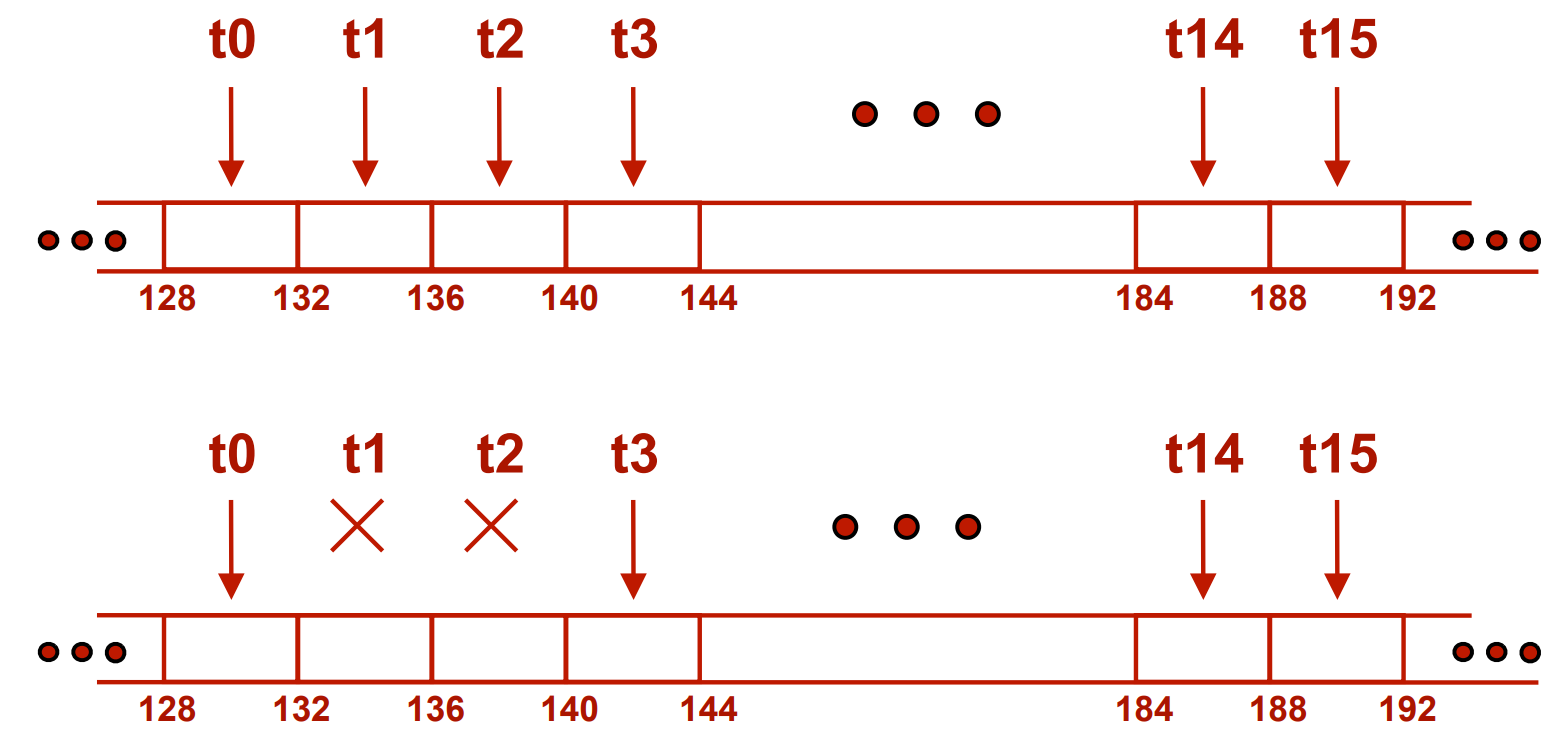
\includegraphics[width=0.7\textwidth, keepaspectratio]{images/ch1/CUDA_global_memory_coalesced_access.png}
	\caption{Coalesced access to global memory. Threads are denoted with \code{t<ID>} and the numbers below the rectangular memory locations are global memory addresses. In the upper image, all threads of the warp access successive memory addresses which house words of size 4 bytes (\code{float}), the size of the memory transaction is 64 bytes, and the segment is aligned to its size so that the first address is a multiple of its size: segment is 64 bytes and the starting address is 128: $ 128/64 = 2 $. The lower image shows an example where two threads from the 16-thread warp do not access data. Thus, threads of the warp have two separate execution paths (thread/warp divergence) that are executed sequentially. However, from a memory standpoint, the access is still coalesced as all requirements are fulfilled. Taken from Martínez Manuel Ujaldón's \emph{CUDA Optimizations, Debugging and Profiling} \cite{xUOrKLpxlGjvTonr}.}
	\label{Figure:theory-CUDA-global-memory-coalesced-access}
\end{figure}

\begin{figure}[ht!]
	\centering
	\begin{subfigure}{\textwidth}
		\centering
		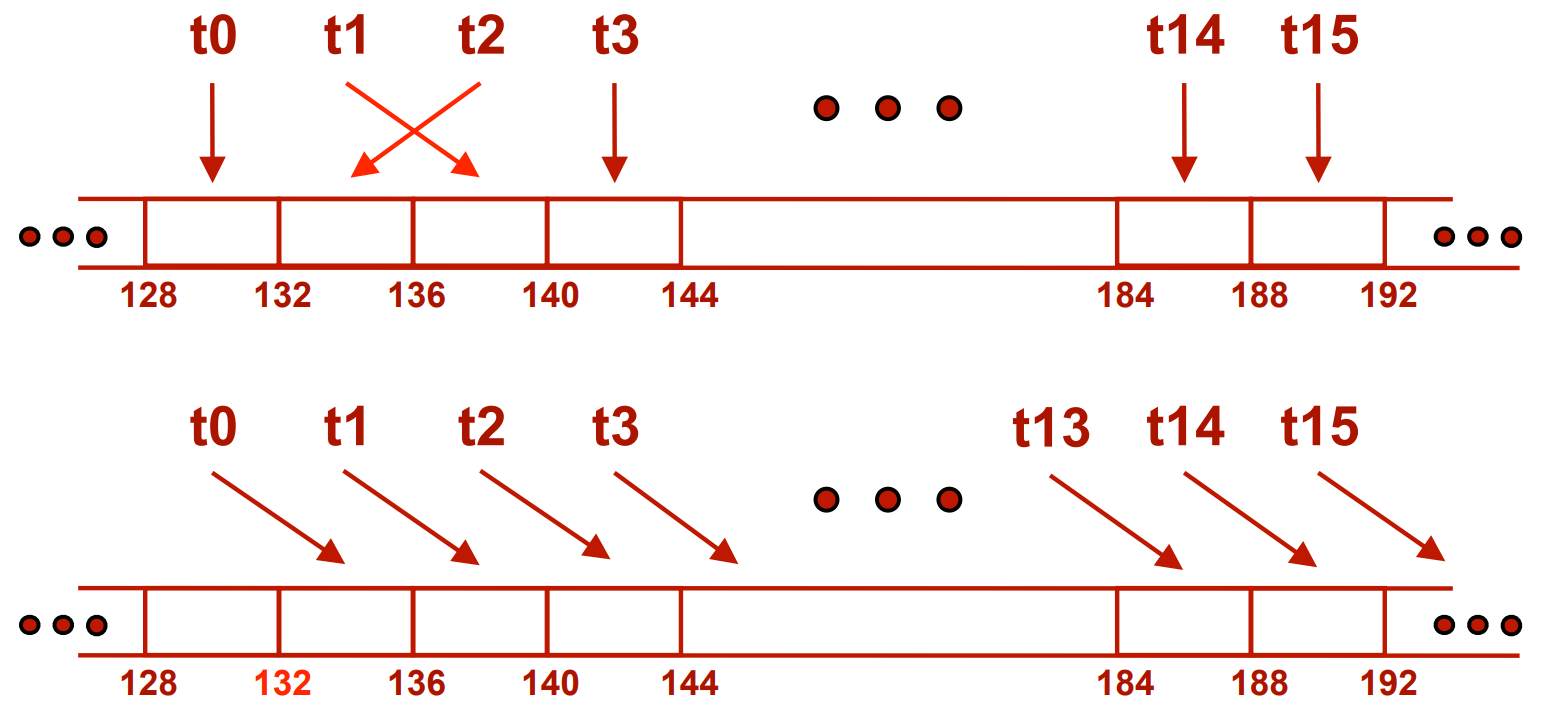
\includegraphics[width=0.7\textwidth, keepaspectratio]{images/ch1/CUDA_global_memory_non-coalesced_access.png}
		\subcaption{In the upper image, two threads swap orders and thus do not access successive floats in global memory. However, according to \emph{CUDA C++ Programming Guide} \cite{NVIDIAMay2022} this does not result in non-coalesced memory access. All other requirements are fulfilled. The lower image shows a scenario where the starting address is misaligned as the size of the memory segment is 64 bytes, but, the starting address is 132 which is not divisible by 64: $ 132/64 = 2.0625 $. Therefore, access is misaligned and the memory segment is read in two sequential memory transactions: starting addresses 128 - 188 and starting addresses 192-252.}
		\label{Sub-figure:theory-CUDA-global-memory-non-coalesced-access}
	\end{subfigure}
	
	\begin{subfigure}{\textwidth}
		\centering
		\hspace*{-0.8cm}
		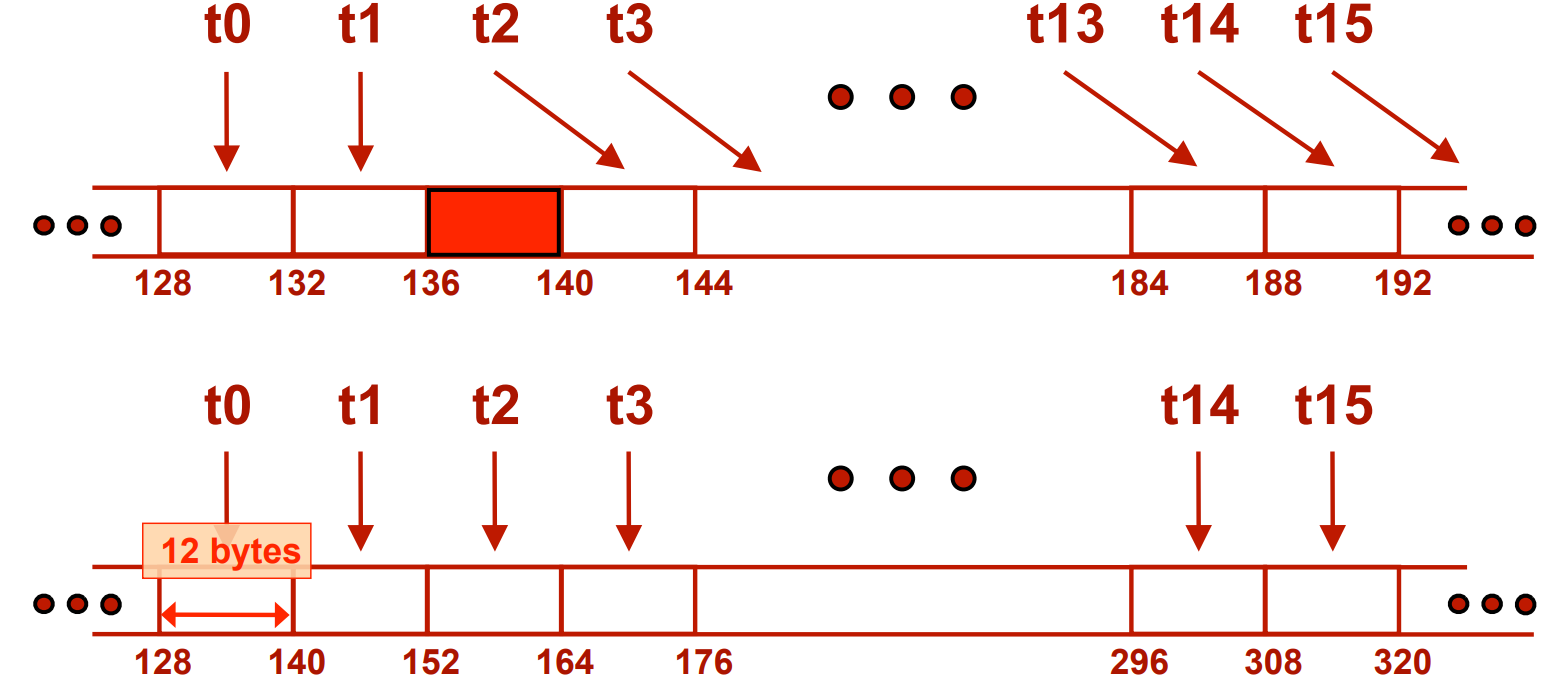
\includegraphics[width=0.7\textwidth, keepaspectratio]{images/ch1/CUDA_global_memory_non-coalesced_access-2.png}
		\subcaption{In the upper image, threads \code{t2} - \code{t15} are misaligned with the original starting address. Thus, similarly to the lower image in Figure~\ref{Sub-figure:theory-CUDA-global-memory-non-coalesced-access} the memory transaction will be split into two sequential transactions. The lower image shows a situation where global memory houses 12-byte \code{struct} types. However, as Table~\ref{Table:theory-CUDA-built-in-aligned-vector-types} and Listing~\ref{Listing:theory-CUDA-aligned-structure-declaration} show, 12-byte alignment is not supported and therefore global memory access is non-coalesced.}
		\label{Sub-figure:theory-CUDA-global-memory-non-coalesced-access-2}
	\end{subfigure}
	\caption{Examples of coalesced and non-coalesced access to global memory composed of 4-byte words (for example, \code{float}) with one exception being 12-byte structures. Taken from Martínez Manuel Ujaldón's \emph{CUDA Optimizations, Debugging and Profiling} \cite{xUOrKLpxlGjvTonr}.}
	\label{Figure:theory-CUDA-global-memory-non-coalesced-access-examples}
\end{figure}

In summary, coalesced access (reading and writing) to global memory must be fulfilled in order to not lower bandwidth - especially when dealing with custom non-built-in vector types - as global memory is implicitly high-latency and low-bandwidth compared to other memory types mentioned above.

\paragraph{Page-locked host memory}\label{Paragraph:theory-CUDA-memory-management-page-locked-host-memory}
This type of memory that can be utilized within CUDA is different from the previous types in that it is not located on the device. Page-locked host memory - sometimes referred to as pinned - resides in the memory of the host. The difference between it and the host's regular pageable memory is its permanent placement and other properties related to CUDA. Firstly, it can be allocated and deallocated using functions that come with CUDA: \code{cudaHostAlloc()} and \code{cudaFreeHost()}, or, if the memory on the host has already been allocated using \code{malloc()} it can be registered - made available within cuda - using \code{cudaHostRegister()}. According to \emph{CUDA C++ Programming Guide} \cite{NVIDIAMay2022} there are many advantages to using page-locked host memory:

\begin{itemize}
	\item Concurrent data transfer between page-locked host memory and device memory, and kernel execution - so-called \textit{asynchronous concurrent execution} (detailed in Section~\ref{Subsection:theory-CUDA-asynchronous-concurrent-execution}).
	\item Elimination of data copying between the host and device by mapping page-locked host memory to the device's address space - so-called \textit{mapped memory} (detailed below).
	\item Higher bandwidth when copying between page-locked host memory and device memory on systems with a front-side bus. Furthermore, if the page-locked host memory is allocated using the write-combining principle, then bandwidth can be even higher.
\end{itemize}

Along with the above-mentioned advantages there are drawbacks such as, the small size of page-locked host memory. Since it is often used by the operating system for paging (host stores data - to-be-used in main memory - in paged memory on a drive rather than in RAM) it is not an abundant resource. Therefore, incautious use can lead to allocation failures and reduced system performance \cite{NVIDIAMay2022}.

\subparagraph{Mapped memory}
As mentioned above one of the advantages of using page-locked host memory is the ability to map this type of memory to the device's address space which eliminates the need for copying data stored in this memory between the host and the device. Specifically, a block of page-locked host memory can be mapped to the device's address space by passing either the \code{cudaHostAllocMapped} flag to \code{cudaHostAlloc()}, or, the \code{cudaHostRegisterMapped} flag to \code{cudaHostRegister()} \cite{NVIDIAMay2022}. \\
Then, the block will have an address in host memory - given by \code{cudaHostAlloc()} (or \code{malloc()}) - and another in device memory. The address in device memory is accessible by using the function \code{cudaHostGetDevicePointer()}, which will provide a pointer that can be used in kernels. Even though this specific type of host memory is accessible from within a kernel, it is not stored on the device and, thus, accessing it is not as fast as accessing device memory. \\
Another advantage of using mapped memory is that copying the block of data between device memory and mapped host memory is done implicitly by kernels when needed, thus, the need to allocate a block in device memory is removed. However, a disadvantage of this characteristic is the potential read-after-write, write-after-read, or write-after-write complications that can arise when asynchronous concurrent execution (detailed in Section~\ref{Subsection:theory-CUDA-asynchronous-concurrent-execution}) is used \cite{NVIDIAMay2022}. These problems can be avoided by forcing memory synchronizations, however, this can have an impact on performance. \\
Further caveats associated with the use of mapped memory can be found in \emph{CUDA C++ Programming Guide} \cite{NVIDIAMay2022}.

\par An overview of how the structure of hardware on a GPU and CUDA can be seen in Figure~\ref{Figure:Nvidia-GPU-structure-CUDA-thread-structure}

\begin{figure}[ht!]
	\centering
	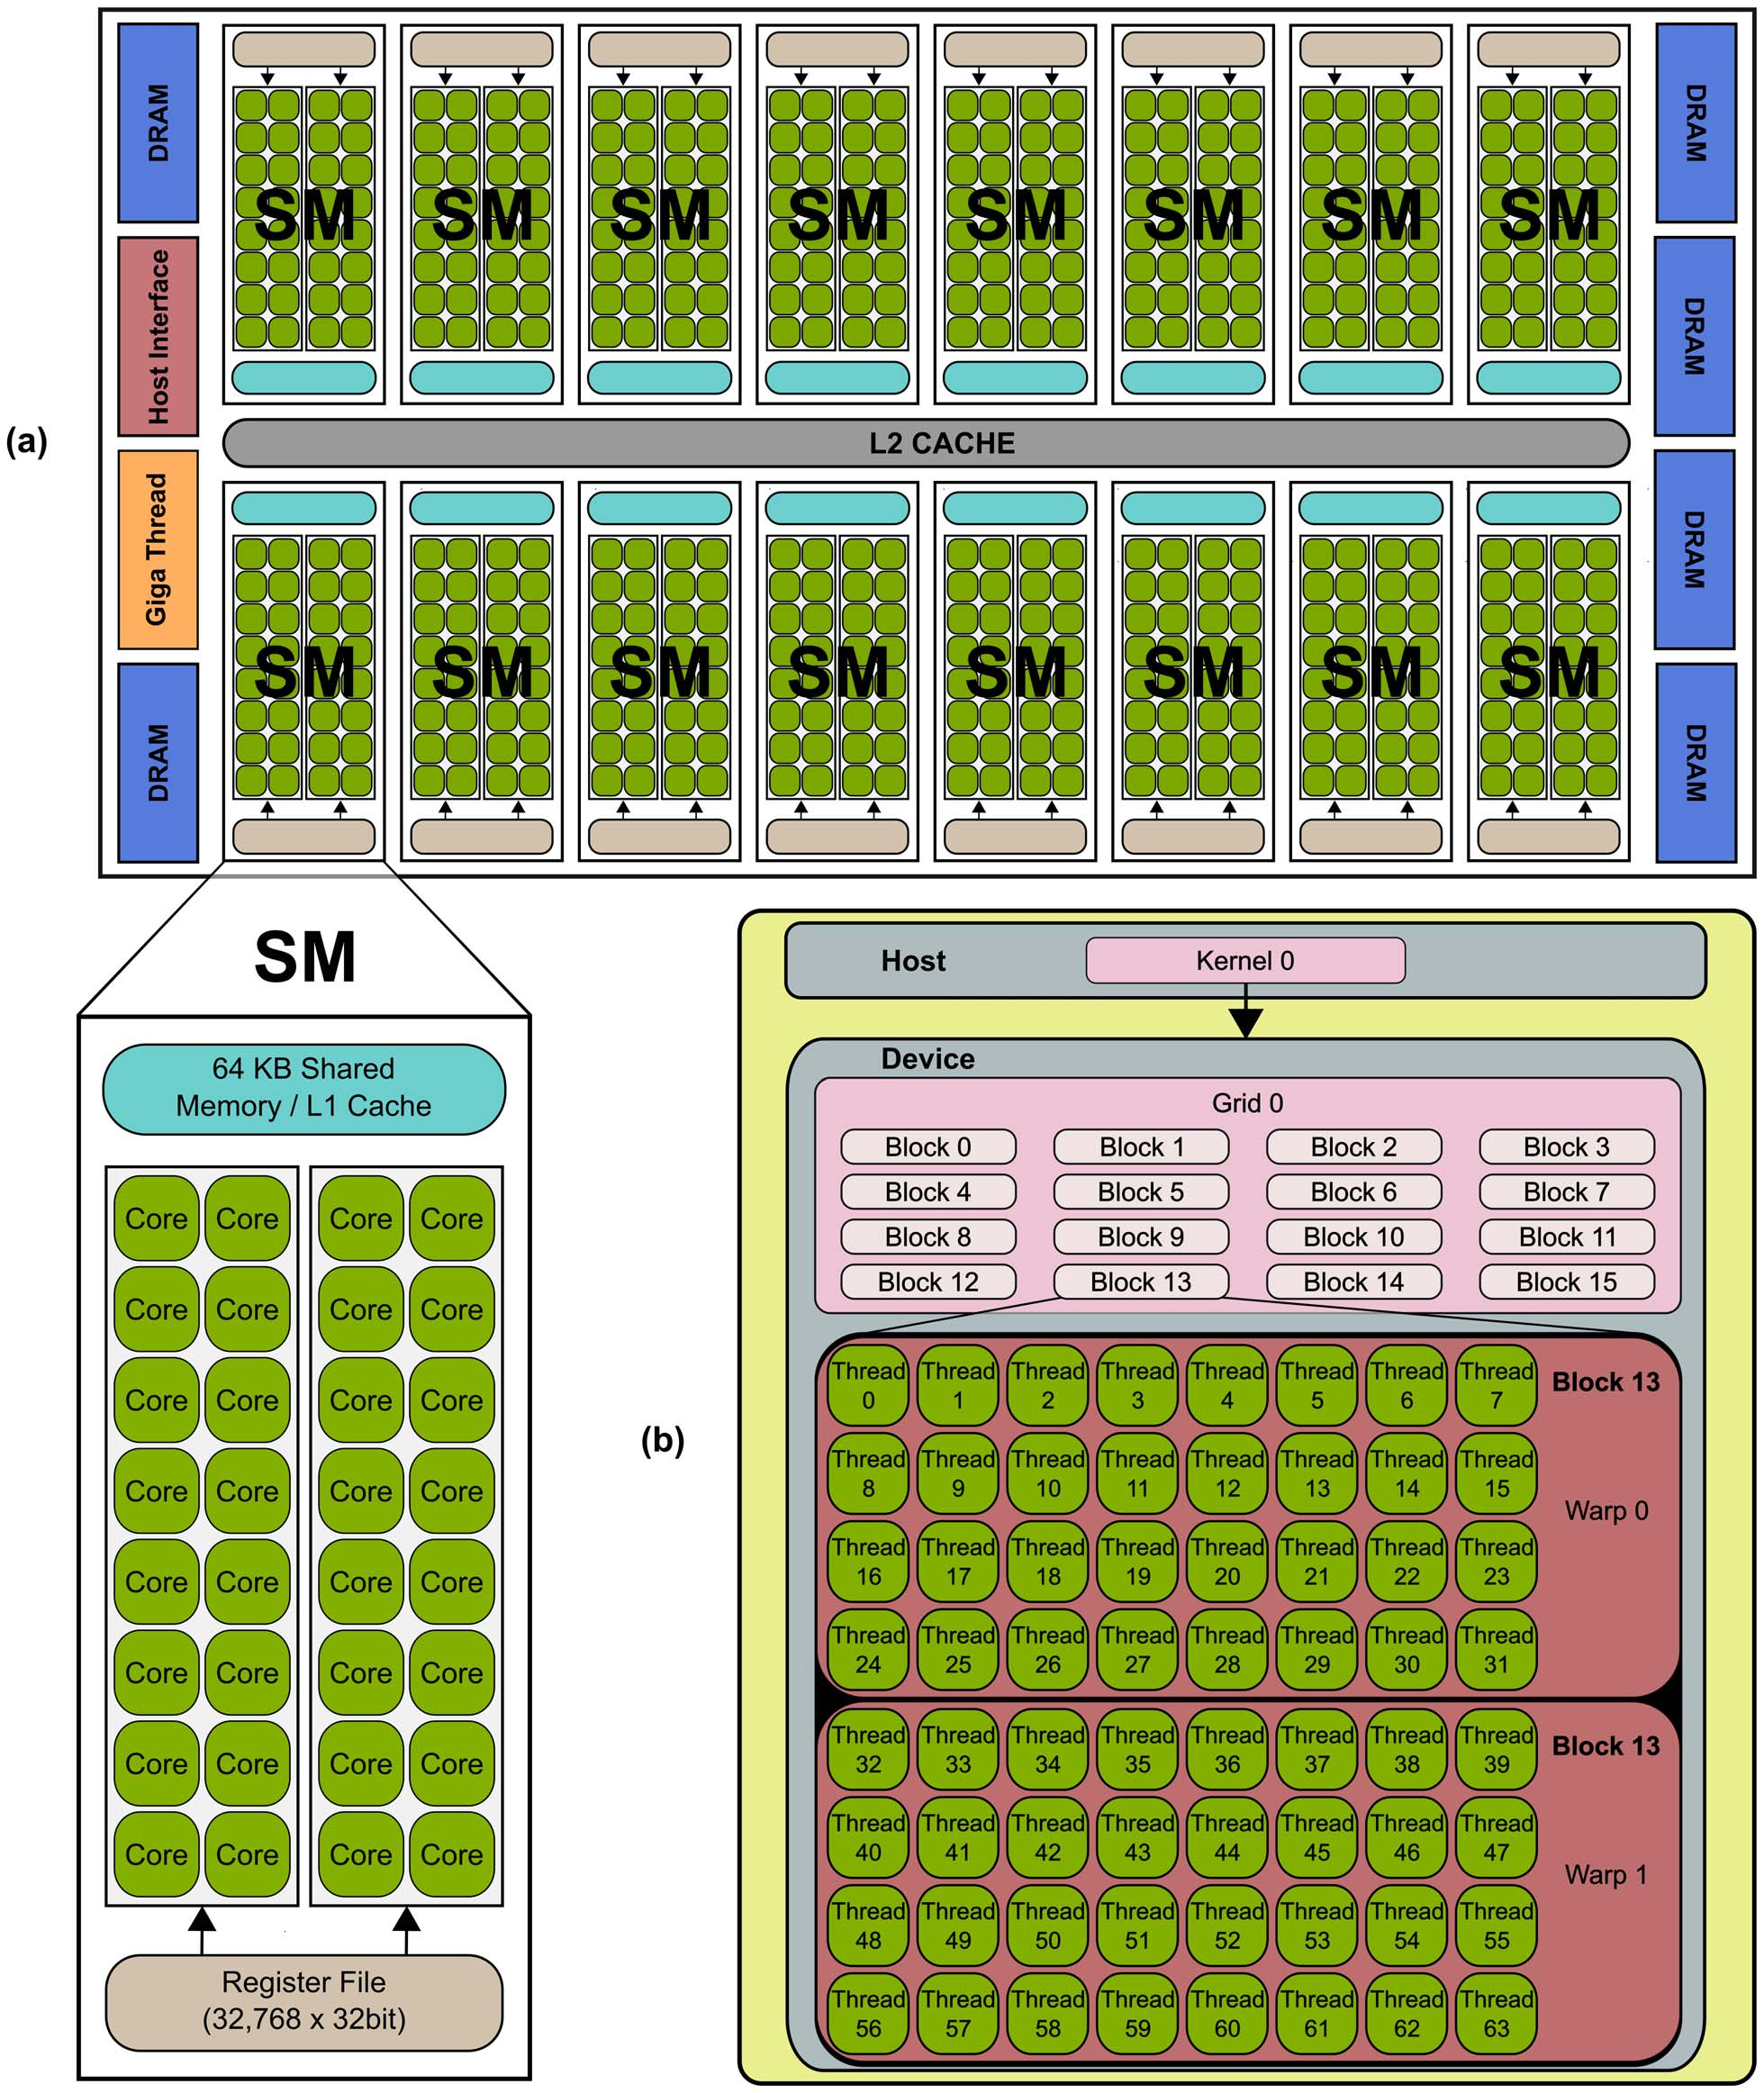
\includegraphics[width=\textwidth, keepaspectratio]{images/ch1/nvidia_gpu_sms_cuda.png}
	\caption{a) Usual architecture of an Nvidia Fermi GPU that comprises of SMs. Furthermore, each SM is made up of SP cores (Stream Processor cores) b) CUDA programming model controls the hardware of the GPU. Taken from \emph{Accelerating Fibre Orientation Estimation from Diffusion Weighted Magnetic Resonance Imaging Using GPUs} \cite{Hernandez2013429}.}
	\label{Figure:Nvidia-GPU-structure-CUDA-thread-structure}
\end{figure}

\subsection{Asynchronous Concurrent Execution}\label{Subsection:theory-CUDA-asynchronous-concurrent-execution}
Within CUDA there are multiple operations that can be executed at the same time (concurrently) - namely \cite{NVIDIAMay2022}:
\begin{itemize}
	\item Computation on the host
	\item Computation on the device
	\item Memory transfers from the host to the device and vice versa
	\item Memory transfers within the memory of a given device
\end{itemize}

However, it is important to note that there is a limit to concurrent load. According to \emph{CUDA C++ Programming Guide} \cite{NVIDIAMay2022} the so-called \textit{level of concurrency} is determined by the compute capability version of the device and its available feature set as detailed below. \\
This section will describe concurrent execution from different perspectives that are used in this project. Firstly, concurrent execution between the host and the device will be presented. Then, concurrent kernel execution will be introduced in greater detail and finally, the topic of streams will be described.
 
\paragraph{Concurrent execution between host and device}
Concurrent host execution means that once the host launches a kernel on the device, then it does not have to wait for the kernel to complete before moving on to the next instruction. CUDA has asynchronous library functions that make the host a controller which essentially sends computation jobs to the device. In other words, once a kernel is launched on the device, the host reclaims control immediately without waiting for the kernel to finish. This means that the host can go on to execute the next line of code. \\
Due to the asynchronous nature, this functionality is especially useful when it comes to queuing job for the device. The jobs are executed on the device by CUDA as soon as sufficient resources are available. Subsequently, the responsibility of managing the device is lifted from the host - allowing it to perform other tasks \cite{NVIDIAMay2022}. \\
Host asynchrony is available for the following device operations \cite{NVIDIAMay2022}:

\begin{itemize}
	\item Kernel launches
	\item Memory copies (only page-locked host memory):
	\begin{itemize}
		\item Within a single device's memory
		\item From host to device - memory block with a limited size of 64 KB
		\item Performed by functions suffixed with \code{Async}
	\end{itemize}
	\item Memory set function calls
\end{itemize}

Asynchronous concurrent execution between host and device can be disabled on a system for all CUDA applications (kernel launches) by using the \code{CUDA\_LAUNCH\_BLOCKING} environment variable (set to \code{1}). However, Nvidia does not recommend using this feature in production - only during debugging. \\
Another noteworthy aspect is that kernel launches are implicitly synchronous when running a CUDA application via a profiler, for example, the Nvidia Visual Profiler. This behavior can be overridden in the profiler by explicitly enabling concurrent kernel profiling \cite{NVIDIAMay2022}.

\paragraph{Concurrent kernel execution}\label{Paragraph:theory-CUDA-asynchronous-concurrent-execution-concurrent-kernel-execution}
Similarly to the concept where the device can be running a kernel while the host is performing another task, kernels can be executed simultaneously on the device. Not all Nvidia devices support this functionality (only some devices with compute capability 2 and higher), therefore, it must be checked per-device using the \code{asyncEngineCount} device property (\code{0} if the device supports it). There are 3 main limitations when it comes to concurrent kernel execution: CUDA-defined maximum number of resident grids per device, no concurrent kernels from different CUDA contexts and resources available on the device. First, the CUDA-defined maximum resident grids per device will be explained. \\
Since each kernel is launched on an individual grid of blocks of threads, then the maximum number of resident grids per device is effectively the maximum number of kernels that can be run concurrently on the device. The limit is a hard-set constant that depends on the compute capability version - Table~\ref{Table:theory-CUDA-maximum-resident-grids-per-device}.

\begin{table}[ht!]
	\centering
	\renewcommand{\arraystretch}{1.5}
	\begin{tabular}{ |c|c|c|c|c|c|c|c|c| } 
		\hline
		Compute Capability & 3.5 - 5.2 & 5.3 & 6.0 & 6.1 & 6.2 & 7.0 & 7.2 & 7.5 - 8.7 \\
		\hline
		Max. resident grids per device & 32 & 16 & 128 & 32 & 16 & 128 & 16 & 128 \\
		\hline
	\end{tabular}
	\caption{Maximum number of resident grids per device depending on the CUDA compute capability version. Taken from Nvidia's \emph{CUDA C++ Programming Guide} \cite{NVIDIAMay2022}.}
	\label{Table:theory-CUDA-maximum-resident-grids-per-device}
\end{table}

The second limitation - CUDA context - signifies that if there are two CUDA applications running at the same time on a system, then two kernels - one from each context - will not be run in concurrently. Instead, the kernel that was launched second will be queued to execute until the first kernel has finished. \\
The last limitation - device resources - is not as severe the previous two since kernels can still be launched concurrently, even if their cumulative required resources exceed the device's available resources. This is due to the fact that if more than one kernel is set to be launched concurrently, they are only run simultaneously if the available resources are sufficient for them all. If the resources available are not sufficient, then the kernels which would not get their requested resources are put aside until the resources are free. In this instance, resources represent memory and threads. \\
In terms of memory, an example of kernels that will often not run concurrently with other kernels are ones that require large amounts of local memory \cite{NVIDIAMay2022}. In terms of threads, the limiting factor is the maximum number of active threads - described at the end of the \textit{\nameref{Paragraph:theory-CUDA-thread-management-grid}} paragraph in Section~\ref{Paragraph:theory-CUDA-thread-management-grid}. For example, if two kernels are to be run concurrently, the total number of threads required by them at once must not exceed the maximum number of active threads on the device. \\
Therefore, whether kernels can be run concurrently is highly dependent on the resource requirements of each kernel and it is up to the device to manage all of these operations.

\subsubsection{Streams}\label{Subsubsection:theory-CUDA-asynchronous-concurrent-execution-concurrent-streams}
Streams can be used to effectively create and manage concurrency on the device, in other words, they are the means by which the above-mentioned operations are controlled. According to \emph{CUDA C/C++ Streams and Concurrency} by Steve Rennich and Nvidia a CUDA \textit{stream} can be defined as "A sequence of operations that execute in issue-order on the GPU" \cite{sk7jHd5INXJOAEUe}. To put it another way, a single stream is basically an open door through which instructions can be sent to the device - kernels. \\
While it is possible to have multiple streams active at once, the device has limited resource available (active threads and memory). Therefore, multiple active streams at once does not necessarily mean multiple kernels running simultaneously. Nevertheless, if multiple streams are active and each is given a different kernel, then these kernels can be executed concurrently if the device's limits are not overstepped - detailed above in paragraph \textit{\nameref{Paragraph:theory-CUDA-asynchronous-concurrent-execution-concurrent-kernel-execution}} in Section\ref{Paragraph:theory-CUDA-asynchronous-concurrent-execution-concurrent-kernel-execution}. \\
Unlike individual kernels, global memory is used by all streams without division, i.e. all streams have access to the same global memory and there is no part of global memory that would belong to a particular stream. \\
According to Nvidia's \emph{CUDA C++ Programming Guide} \cite{NVIDIAMay2022}, individual streams are not dependent on each other, meaning that they are able to execute commands separately or concurrently. However, this behavior does not have to be consistent, for example, communication between kernels is not define. For this reason, Nvidia themselves recommend not relying on the accuracy of CUDA applications when attempting to make streams interact. \\
On the other hand, CUDA provides tools that can assist when synchronicity of streams is required. \\
This section will first present basic information on stream creation and destruction. Then, the topic of the default CUDA stream will follow and, finally, explicit and implicit synchronization will be detailed.

\paragraph{Creation and destruction}
A CUDA stream is created by initializing a stream object - type \code{cudaStream\_t} in code - and then creating the stream itself using \code{cudaStreamCreate()}. The approach that is often used in examples by Nvidia is to create an array of streams as shown in Listing~\ref{Listing:streams-creation}.

\begin{lstlisting}[caption={Creation of streams. Taken from Nvidia's \emph{CUDA C++ Programming Guide} \cite{NVIDIAMay2022}.},label={Listing:streams-creation}]
// Declare array of 2 stream objects
cudaStream_t streams[2];

// Create each stream
for( int i = 0; i < 2; ++i ) {
	cudaStreamCreate( &streams[i] );
}
\end{lstlisting}

In order to make a kernel run on a specific stream, the stream address must be specified as one of the launch parameters of the kernel - detailed in Section~\ref{Subsection:theory-CUDA-C++-extensions}. Launching a kernel on a specific stream is shown in Listing~\ref{Listing:run-kernels-on-streams}.

\begin{lstlisting}[caption={Pseudo-code for launching two different kernels using two different streams. The instructions in this example would be executed from the host. Since each kernel is essentially an open door to the device for instructions, then, once \code{MyKernelA} is launched on \code{stream[0]}, the control is returned to the host without waiting for \code{MyKernelA} to finish. Subsequently, the host will immediately launch \code{MyKernelB} using \code{stream[1]}. In this example, each kernel is launched on a grid made up of one single-thread block with 0 bytes of dynamic shared memory allocated, thus, the devic resources will not be exhausted and both kernels will run concurrently. Taken from Nvidia's \emph{CUDA C++ Programming Guide} \cite{NVIDIAMay2022}.},label={Listing:run-kernels-on-streams}]
// Launch MyKernelA using the 0th stream using 1 block made up of 1 thread and 0 bytes of dynamically allocated shared memory
MyKernelA<<< 1, 1, 0, stream[0] >>>( inputVariableA )

// Launch MyKernelB using the 1st stream
MyKernelB<<< 1, 1, 0, stream[1] >>>( inputVariableB )
\end{lstlisting}

When streams are no longer needed, they are to be destroyed using \code{cudaStreamDestroy()} - show below in Listing~\ref{Listing:streams-destruction}. If \code{cudaStreamDestroy()} is called while a stream is still performing tasks, then it will return without destroying the stream immediately - the destruction (release) of the stream's resources will be delayed until all work is completed on the stream.

\begin{lstlisting}[caption={Destruction of streams. Taken from Nvidia's \emph{CUDA C++ Programming Guide} \cite{NVIDIAMay2022}.},label={Listing:streams-destruction}]
// Destroy each stream
for( int i = 0; i < 2; ++i ) {
	cudaStreamDestroy( stream[i] );
}
\end{lstlisting}

\paragraph{Default stream}\label{Paragraph:theory-CUDA-asynchronous-concurrent-execution-streams-default-stream}
If a stream is not specified when launching a kernel, or when copying memory, then only the default stream - \textit{Stream '0'} - is used and the instruction are executed in order with respect to the device (not concurrently as shown in the examples above) \cite{NVIDIAMay2022}. \\
Nevertheless, it is possible to provide each host thread with its own default stream by setting the \code{----default-stream} compilation flag to \code{per-thread}, i.e. compiling using \code{nvcc ... ----default-stream per-thread}. \\
The default option for the flag is \code{legacy}, which signifies that all host threads will use the special \textit{NULL stream}. This stream is different from other streams as it uses implicit synchronization - detailed below in paragraph~\ref{Paragraph:theory-CUDA-asynchronous-concurrent-execution-streams-implicit-synchronization}.

\paragraph{Explicit synchronization}\label{Paragraph:theory-CUDA-asynchronous-concurrent-execution-streams-explicit-synchronization}
The first, and arguably the most used, type of synchronization when it comes to streams is explicit synchronization. In this instance, the 'explicit' modifier signifies that the synchronization is issued using one of the following functions from code \cite{NVIDIAMay2022, NvidiaJanuary2022}:
\begin{itemize}
	\item \code{cudaDeviceSynchronize()} - Synchronization of the entire device. This function servers as a checkpoint in code where streams will wait until they all get to this point in code.
	\item \code{cudaStreamSynchronize( cudaStream\_t stream )} - Synchronization of a particular stream. This function takes a single \code{stream} as its input parameter and serves a checkpoint to wait the for completion for all actions called before it.
	\item \code{cudaStreamWaitEvent(  cudaStream\_t stream, cudaEvent\_t event )} - Execution delayed for commands added to the input \code{stream} until the input \code{event} completes.
\end{itemize}

Additionally, CUDA provides a function to check whether all commands of a stream that precede the current line of code have finished: \code{cudaStreamQuery()}. Further functions that can be used to manage streams can be found in section \emph{6.4 Stream Management} in the \emph{CUDA Runtime API} \cite{NvidiaJanuary2022}.

\paragraph{Implicit synchronization}\label{Paragraph:theory-CUDA-asynchronous-concurrent-execution-streams-implicit-synchronization}
The opposing type of synchronization is called implicit, and, as mentioned in paragraph \textit{\nameref{Paragraph:theory-CUDA-asynchronous-concurrent-execution-streams-default-stream}} above, it is used by default under certain conditions - unless explicitly overridden by one of the functions above. Specifically, Nvidia states in \emph{CUDA C++ Programming Guide} \cite{NVIDIAMay2022} that if there are two streams, then two commands - each from one stream - cannot be run simultaneously if the host thread issues any of the following operations:

\begin{itemize}
	\item Page-locked host memory allocation
	\item Device memory allocation
	\item Device memory set
	\item Memory copy between two addresses to the same device memory
	\item Any CUDA command to the NULL stream
	\item Switch between the shared memory configurations
\end{itemize}

The hypothetical reasoning behind this is that if any of the operations above would be performed in parallel, it could create irresolvable conflicts. For example, if each stream tried to allocate memory on the device at the same location concurrently - impossible to be done in parallel without a conflict check. However, it can be argued that a conflict check is an unnecessary functionality as it is already present in some form when allocation happens sequentially. \\
Furthermore, there are certain operations that require a dependency check \cite{NVIDIAMay2022}:

\begin{itemize}
	\item Any other commands within the same stream as the launch being checked
	\item Any call to \code{cudaStreamQuery()} on that stream
\end{itemize}

Thus, in order to improve application performance, Nvidia recommends developers issue all independent operations before dependent operations and delay any synchronization until necessary.


\subsection{C++ CUDA Extensions}\label{Subsection:theory-CUDA-C++-extensions}
As previously mentioned at the beginning of Section~\ref{Section:theory-CUDA}, CUDA supports a variety of programming languages. Among them is C++, a widely-used, high-performance C-based language that implicitly allows low-level memory manipulation. CUDA provides many different extensions to C++, however, for the purpose of this project only the core basics that were used during its development along with some other important extensions will be detailed. \\
This section will divided into two main categories: outer-kernel and inner-kernel extensions. The former is made up of memory-related operations (allocating, copying and freeing data), kernel launch configurations, function extensions, streams, etc. - i.e. extensions not used within kernels. The latter consists of any operators, structures and declarations that are used in kernels.

\subsubsection{Outer-kernel Extensions}\label{Subsubsection:theory-CUDA-C++-extensions-outer-kernel-extensions}
This category will first present a selection of important memory managing extensions along with those that were used during the development of this project. Then, kernel-specific extensions will be detailed. Finally, the last part will present function modifiers that state where a function can be executed. The extensions to C++ for streams were described above in the \textit{\nameref{Subsubsection:theory-CUDA-asynchronous-concurrent-execution-concurrent-streams}} part of Section~\ref{Subsubsection:theory-CUDA-asynchronous-concurrent-execution-concurrent-streams}.

\paragraph{Memory managing extensions}\label{Paragraph:theory-CUDA-C++-extensions-outer-kernel-extensions-memory-managing-extensions}
CUDA offers many memory managing extensions to C++, however, there are a select few that are widely used for allocating, copying and freeing data \cite{NVIDIAMay2022, NvidiaJanuary2022, Cejka2020}:

\begin{itemize}
	\item \code{cudaMalloc( void** devPtr, size\_t size )} - Function that allocates \code{size} bytes in device memory and stores the address in the \code{devPtr} pointer. \\
	Note that since the pointer is to an address located in device memory, it is inaccessible from the host - access from the host would first require for the data to be copied using \code{cudaMemcpy()}. \\
	This function is widely used when it comes to allocating anything from single variables to large arrays. \\
	If the data was allocated successfully, then \code{cudaSuccess} is returned, otherwise one of \code{cudaErrorInvalidValue}, \code{cudaErrorMemoryAllocation} is returned - depending on the type of failure.
	\item \code{cudaMemcpy( void* dst, const void* src, size\_t count, }\\ \code{cudaMemcpyKind kind )} - Function that copies \code{count} bytes from the source memory address (\code{src}) to the destination memory address (\code{dst}). The \code{kind} parameter specifies the direction of copying; it has to be one of the following: \code{cudaMemcpyHostToHost}, \code{cudaMemcpyHostToDevice}, \code{cudaMemcpyDeviceToHost}, \code{cudaMemcpyDeviceToDevice}, or \code{cudaMemcpyDefault}. \\
	Similarly to \code{cudaMalloc()}, if the data was copied successfully, then \code{cudaSuccess} is returned, otherwise one of \code{cudaErrorInvalidValue}, \\ \code{cudaErrorInvalidMemcpyDirection} is returned - depending on the type of failure.
	\item \code{cudaFree( void* devPtr )} - Function that frees memory on the device that is pointed to by \code{devPtr}. \\
	If the memory was successfully freed, then \code{cudaSuccess} is returned, otherwise \code{cudaErrorInvalidValue} is returned. \\
	It is also worth noting that in order to be freed using \code{cudaFree()} the memory \code{devPtr} is pointing to must have been allocated by one of CUDA's memory allocation APIs, for example, \code{cudaMalloc()}, \code{cudaMallocAsync()}, etc. - the complete list can be found in Nvidia's \emph{CUDA Runtime API: API Reference Manual} \cite{NvidiaJanuary2022}.
	\item \code{cudaMallocHost( void** ptr, size\_t size )} - Function that allocates \code{size} bytes of page-locked memory on the host and stores the address in the \code{ptr} pointer. The benefits and caveats of using page-locked memory are detailed in paragraph \textit{\nameref{Paragraph:theory-CUDA-memory-management-page-locked-host-memory}} in Section~\ref{Paragraph:theory-CUDA-memory-management-page-locked-host-memory}.
\end{itemize}

Expanding on the memory operations mentioned above, CUDA provides memory space specifiers that can be used to denote in what memory a variable ought to be stored. Among such often-used specifiers are \cite{NVIDIAMay2022}:

\begin{itemize}
	\item \code{\_\_device\_\_} - Memory space specifier declaring that a variable is stored in global memory on the device. Since it resides in global memory, it is accessible by all threads from the grid and it is present for the lifetime of the CUDA application. It is noteworthy that if multiple CUDA devices are present in the system, then a variable with this specifier is a unique object for each device.
	\item \code{\_\_shared\_\_} - Memory space specifier declaring that a variable is stored in shared memory of a thread block. Since it resides in shared memory, it is only accessible by threads of a block as each block has its own unique object of this variable.
\end{itemize}

Listing~\ref{Code:theory-CUDA-memory-managing-extensions-example} shows an example of how memory managing functions can be used in a host-device code that copies arrays.

\begin{lstlisting}[caption= Example of code that utilizes CUDA memory managing extensions of C++. Taken from \emph{Formats for storage of sparse matrices on GPU} \cite{Cejka2020} and Nvidia's \emph{Getting Started with CUDA} presentation \cite{Ruetsch2008}.,label=Code:theory-CUDA-memory-managing-extensions-example]
int main()
{
	float *a_h, *b_h; // data that will be allocated on host
	float *a_d, *b_d; // data that will be allocated on device
	int N = 14, nBytes, i;
	
	nBytes = N * sizeof( float ); // required allocation size
	a_h = (float *) malloc( nBytes ); // allocating host data
	b_h = (float *) malloc( nBytes ); 
	cudaMalloc( (void **) &a_d, nBytes ); // allocating device data
	cudaMalloc( (void **) &b_d, nBytes );
	
	// filling up host data
	for( i = 0, i < N; ++i ) {
		a_h[i] = 100.f + i;
	}

	// copying data from host -> device -> device -> host
	cudaMemcpy( a_d, a_h, nBytes, cudaMemcpyHostToDevice );
	cudaMemcpy( b_d, a_d, nBytes, cudaMemcpyDeviceToDevice );
	cudaMemcpy( b_h, b_d, nBytes, cudaMemcpyDeviceToHost );
	
	// checking that all data is equal
	for( i = 0; i < N; ++i ) {
		assert( a_h[i] == b_h[i] );
	}

	free( a_h ); free( b_h ); // freeing data on host
	cudaFree( a_d ); cudaFree( b_d ); // freeing data on device
	return 0;
}
\end{lstlisting}

\paragraph{Kernels}\label{Paragraph:theory-CUDA-c++-CUDA-extensions-kernels}
While the term \textit{kernel} was introduced earlier in Section~\ref{Subsection:theory-CUDA-introductory-terminology}, the technical details will be covered in this part. In order to differentiate a kernel from a function, the \code{\_\_global\_\_} modifier must be used. Another distinction that kernels have compared to regular functions is the kernel launch configuration which has the following specific syntax: \code{$<$$<$$<$ numBlocks, threadsPerBlock, sharedMemSize,} \code{stream $>$$>$$>$} where \cite{NVIDIAMay2022, Cejka2020}:

\begin{itemize}
	\item \code{numBlocks} specifies the number of blocks in the grid and their structure;
	\item \code{threadsPerBlock} specifies the number of threads per block and their structure;
	\item \code{sharedMemSize} specifies the number of bytes that are to be dynamically allocated in shared memory for each block (on top of any statically allocated shared memory). This argument is not mandatory and its default value is 0;
	\item \code{stream} specifies stream to which the kernel should be sent for execution. This argument is also not mandatory and defaults to 0 - the default stream.
\end{itemize}

The \code{sharedMemSize} parameter is of type \code{size\_t}, \code{stream} is of type \code{cudaStream\_t}, and parameters \code{numBlocks} and \code{threadsPerBlock} can be either of type \code{int} or \code{dim3}. The \code{dim3} type is a 3-dimensional \code{unsigned int} vector used to specify dimensions. It can be defined with up to 3 variables (1 for each dimension) with an implicit dimension value of 1, i.e., if a vector component (dimension) is not specified when declaring a \code{dim3} variable, it is by default initialized to 1. \\
For example, if \code{numBlocks} is of type \code{int}, then the grid is one-dimensional and composed of \code{numBlocks} blocks. Concordantly, if \code{threadsPerBlock} is type \code{int}, then all blocks in the grid will be one-dimensional with \code{threadsPerBlock} threads. \\
On the other hand if \code{threadsPerBlock} is a \code{dim3} variable, then the thread structure of all blocks can be up to three-dimensional. An example of a kernel being called with the properties above can be seen in Listing~\ref{Listing:theory-CUDA-kernel-example}.

\begin{lstlisting}[caption={Example of C++ pseudocode of a Kernel launch on a grid consisting of 1 one-dimensional block that is made up of 8 threads. Taken from Nvidia's \emph{CUDA C++ Programming Guide} \cite{NVIDIAMay2022}.},label={Listing:theory-CUDA-kernel-example}]
// Kernel definition
__global__ void MyKernel( float a, float b, float c )
{
	// Kernel code here
}

int main()
{
	...
	// Kernel invocation on a grid with 1 block of 8 * 1 * 1 threads
	int numBlocks = 1;
	dim3 threadsPerBlock( 8 ); // Defaults to (8, 1, 1)
	MyKernel<<< numBlocks, threadsPerBlock >>>( a, b, c );
	...
}
\end{lstlisting}

\paragraph{Function extensions}\label{Paragraph:theory-CUDA-C++-extensions-outer-kernel-extensions-function-extensions}
In the part above, the \code{\_\_global\_\_} modifier was introduced as a specifier for functions that are to be considered kernels. Along with it, CUDA brings other function modifiers, or, as Nvidia calls them: \textit{execution space specifiers} \cite{NVIDIAMay2022}:

\begin{itemize}
	\item \code{\_\_global\_\_} - Modifier declaring that a function can be called from both the host and the device (as of compute capability 3.2 or higher). However, it can only be executed on the device. Additionally, a function denoted with this modifier must not belong to any class and it can only have a void return type. Furthermore, the launch configuration mentioned above in the \textit{\nameref{Paragraph:theory-CUDA-c++-CUDA-extensions-kernels}} paragraph must be specified for each call.
	\item \code{\_\_device\_\_} - Modifier declaring that a function can only be called from and executed on the device. This means that it can only be called from within kernels.
	\item \code{\_\_host\_\_} - Modifier declaring that a functions can only be called from and executed on the host. This means that it can only be called from regular functions, not kernels.
\end{itemize}

If no modifier is included for a function, it is compiled for the host only. However, if both \code{\_\_device\_\_} and \code{\_\_host\_\_} are specified for a function, then it is compiled both for the host and for the device. The complete list of modifiers can be found in \emph{CUDA C++ Programming Guide} \cite{NVIDIAMay2022}.

\subsubsection{Inter-kernel Extensions}\label{Subsubsection:theory-CUDA-C++-extensions-inter-kernel-extensions}
This category comprises of variables, structures and operations etc. that are most often used within a kernel. First, the means by which developers are able to identify individual threads will be detailed. Then, different memory-type identifiers will be briefly presented along with established operations used to avoid erroneous behaviors in kernels.

\paragraph{Thread identification}
Once a kernel is a launched on the device, it can be run concurrently on thousands of threads. This presents a scenario where the developer must distinguish what each thread will perform within the kernel. For this purpose, the following variables - among others - are available within every kernel for each thread \cite{NVIDIAMay2022}:

\begin{itemize}
	\item \code{threadIdx} - ID of a thread within a block stored in a 3-component vector (1 component for each of 3 dimensions). For example, if the thread block is 2-dimensional, then \code{threadIdx.x} stores the thread's ID in the first dimension and \code{threadIdx.y} stores the thread's ID in the second dimension - the pair of IDs is unique only within the thread's block.
	\item \code{blockIdx} - ID of a block within a grid stored in a 3-component vector (1 component for each of 3 dimensions). Similarly to \code{threadIdx}, the block's ID in the first dimension is retrieved using \code{blockIdx.x}, the second using \code{blockIdx.y} and the third using \code{blockIdx.z}. Within a kernel, the block ID refers to the block of threads that the executing thread belongs to.
	\item \code{blockDimx} - Dimensions of a thread's block stored in a 3-component vector (1 component for each of 3 dimensions). For example, for a block made up of \code{32x16x2} threads: \code{blockDimx.x = 32}, \code{blockDimx.y = 16} and \code{blockDimx.z = 2}.
\end{itemize}

The variables above can be combined to calculate the global ID of a thread, i.e. the thread's ID within a grid:
$$\code{globalID = blockIdx.x * blockDimx.x + threadIdx.x}$$
The \code{globalID} is useful when working with matrices, for example, adding two matrices. In such an example, each thread would take two elements (1 from each matrix), add them and then store the result into a new matrix - as shown in Listing~\ref{Listing:theory-CUDA-matrix-addition-example}.

\begin{lstlisting}[caption={Example of C++ pseudocode of a kernel that adds two matrices using 2-dimensional thread blocks. Since each thread has a unique \code{globalID} for each of two dimensions, then those IDs can be used as indices for adding matrix elements. This simple example does not take into account allocation and copying data from host to device. Taken from Nvidia's \emph{CUDA C++ Programming Guide} \cite{NVIDIAMay2022}.},label={Listing:theory-CUDA-matrix-addition-example}]
// Kernel definition
__global__ void MatAdd( float A[N][N], float B[N][N], float C[N][N] )
{
	// Get thread ID for each dimension -> use as matrix indices
	int i = blockIdx.x * blockDim.x + threadIdx.x;
	int j = blockIdx.y * blockDim.y + threadIdx.y;
	
	// Check if the IDs are within the dimensions of the matrices
	if( i < N && j < N ) {
		C[i][j] = A[i][j] + B[i][j];
	}
}

int main()
{
	...
	// Number of threads per each 2-dimensional block is 16x16 = 256
	dim3 threadsPerBlock( 16, 16 );
	
	// Number of blocks in the grid depends on the matrix dimension (NxN)
	dim3 numBlocks( N / threadsPerBlock.x, N / threadsPerBlock.y );
	
	// Kernel launch: A + B = C
	MatAdd<<< numBlocks, threadsPerBlock >>>( A, B, C );
	...
}
\end{lstlisting}

Accompanying the code in Listing~\ref{Listing:theory-CUDA-matrix-addition-example}, Figure~\ref{Figure:theory-CUDA-GridBlockThread-Structure} visualizes how elements of a matrix can be divided into a grid comprising of 2-dimensional thread blocks.

\begin{figure}[ht!]
	\centering
	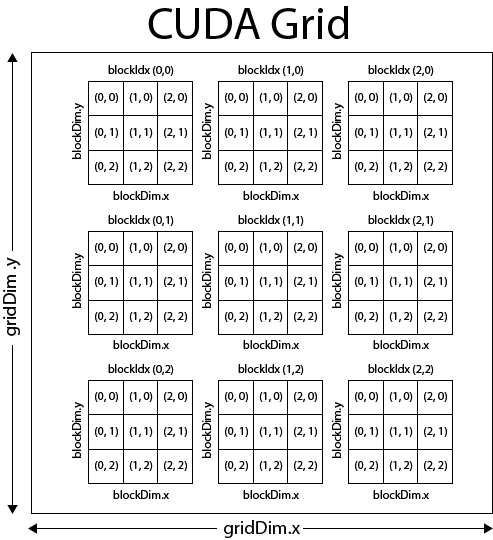
\includegraphics[width=0.8\textwidth, keepaspectratio]{images/ch1/CUDA-GridBlockThread-Structure.png}
	\caption{Grid made up of 2-dimensional thread blocks. Each square represents a thread with its IDs within its block (\code{threadIdx.x}, \code{threadIdx.y}). It can be imagined that each block is a submatrix and together all submatrices make up the full matrix. Taken from \emph{CUDA Parallel Thread Management} \cite{McKennon13June2013}.}
	\label{Figure:theory-CUDA-GridBlockThread-Structure}
\end{figure}

Finally, as mentioned in paragraph \textit{\nameref{Paragraph:theory-CUDA-memory-management-global-memory}} in Section~\ref{Paragraph:theory-CUDA-memory-management-global-memory}, the coalesced access of threads effectively means that neighboring threads access global memory. To add to this, it is important to mention that threads are considered neighboring in the first dimension. In other words, neighbors according to \code{threadIdx.x} values.

\paragraph{Memory specifiers and other operations}
Some memory space specifiers described in above in paragraph \textit{\nameref{Paragraph:theory-CUDA-C++-extensions-outer-kernel-extensions-memory-managing-extensions}} in Section~\ref{Paragraph:theory-CUDA-C++-extensions-outer-kernel-extensions-memory-managing-extensions} can be used within kernels, specifically the \code{\_\_shared\_\_} specifier. Its use within kernels is mostly related to statically allocated shared memory where the size of the variable or array is known during compilation \cite{NVIDIAMay2022}. An example showing this use of the specifier can be seen in Listing~\ref{Listing:theory-CUDA-matrix-multiplication-with-shared-memory-example}. \\
In paragraph \textit{\nameref{Paragraph:theory-CUDA-memory-management-shared-memory}} in Section~\ref{Paragraph:theory-CUDA-memory-management-shared-memory}, it was mentioned that threads of a block are able to share data purely among each other. However, this advantage can also bring problems, such as, some threads overwriting data that other threads have not finished using, or, some threads reading data that other threads have not yet written - known as a \textit{race condition} \cite{Harris28January2013}. CUDA addresses this issue by enabling the synchronization of threads in a block which can be done by calling the built-in function: \code{\_\_syncthreads()}. This function can seen as a meeting checkpoint for all threads of a particular block, i.e., threads of a block will wait at this point until every single thread in their block has finished their work until this point. To put it more clearly: threads of a block are halted on the the line in code that contains \code{\_\_syncthreads()} until all threads of the block arrive to at it \cite{NVIDIAMay2022}.


\subsection{Matrix Multiplication}\label{Subsection:matrix-multiplication}
In order to consolidate how CUDA can be used to accelerate the execution of a simple task, such as matrix multiplication, this section will present solutions to this task from Nvidia's \emph{CUDA C++ Programming Guide} \cite{NVIDIAMay2022}. Furthermore, for the purpose of showcasing and stressing the importance of abiding by Nvidia's recommendations when it comes to best practices and optimal performance, two examples will be presented. The first example will only use global memory to read the input matrix and write the resulting matrix, i.e. without shared memory. On the other hand, the second example will use shared memory to minimize accessing global memory. \\
It is important to note that neither example is fully functional as the logic of some functions has been omitted due to unnecessary complexity and irrelevance to showcasing the capabilities of CUDA. In other words, the code shown will not compile, nor will it run - the full code can be found in Nvidia's \emph{CUDA C++ Programming Guide} \cite{NVIDIAMay2022}. The full working example (\code{matrixMul.cu}) encompassed by the build automation tool \code{make} can be unpacked during the installation of a CUDA toolkit. \\
Before introducing the specifics of each example, their similarities will be presented. \\
First, the task that will be performed is matrix multiplication:

\begin{equation}\label{Equation:matrix-multiplication-definition}
	\mathbb{C} = \mathbb{A} \cdot \mathbb{B} \,.
\end{equation}

In the context of this operation all matrix dimensions are assumed such that it is a legal operation. Additionally, for simplicity, the dimensions of the matrices are assumed to be multiples of the thread block size. This limitation can be avoided by allocating an extra row and column of blocks in the grid and setting a boundary condition in the kernel - each of the two examples (global vs shared memory) require slightly different approaches which will be described later. \\
Let each matrix be represented by a structure \code{Matrix}:

\begin{lstlisting}[caption={Definition of the structure that will represent a matrix. The \code{width} variable stores the number of columns and \code{height} stores the number of rows the matrix has. The elements of the matrix are stored in row-major order in the single-precision (float) array: \code{values}. Taken from Nvidia's \emph{CUDA C++ Programming Guide} \cite{NVIDIAMay2022}.},label={Listing:theory-CUDA-matrix-multiplication-matrix-structure-definition}]
// Matrices are stored in row-major order:
// M( row, col ) = *( M.values + row * M.width + col )
typedef struct {
	int width;
	int height;
	float* values;
} Matrix;
\end{lstlisting}

Furthermore, let there be a host function \code{MatMul} that will:

\begin{enumerate}
	\item Take matrices $ \mathbb{A} $, $ \mathbb{B} $, $ \mathbb{C} $ from Equation~\ref{Equation:matrix-multiplication-definition} as input structures: \code{A}, \code{B}, \code{C}.
	\item Allocate memory for the matrix structures on the device.
	\item Copy the matrix structures from host to device memory.
	\item Invoke the matrix multiplication kernel with a constant thread block size set at compile time.
	\item Copy the resulting matrix from device to host memory.
	\item Free previously allocated memory from the device.
\end{enumerate}

Listing~\ref{Listing:theory-CUDA-matrix-multiplication-host-mat-mul-function} shows the implementation of the points mentioned above.

\begin{lstlisting}[caption={Definition of the function that will allocate and copy all matrices to the device, invoke the kernel and then free the device memory. The size of the thread block is constant and set during compile time using the \code{\#define} macro. Taken from Nvidia's \emph{CUDA C++ Programming Guide} \cite{NVIDIAMay2022}.},label={Listing:theory-CUDA-matrix-multiplication-host-mat-mul-function}]
// Thread block size - 16x16 = 256 threads
#define BLOCK_SIZE 16

// Matrix multiplication - Host code
// Matrix dimensions are assumed to be multiples of BLOCK_SIZE
void MatMul( const Matrix A, const Matrix B, Matrix C )
{
	// Allocate and copy A to device memory
	Matrix d_A;
	d_A.width = A.width; d_A.height = A.height;
	size_t size = A.width * A.height * sizeof(float);
	cudaMalloc( &d_A.values, size );
	cudaMemcpy( d_A.values, A.values, size, cudaMemcpyHostToDevice );
	
	// Allocate and copy B to device memory
	Matrix d_B;
	d_B.width = B.width; d_B.height = B.height;
	size = B.width * B.height * sizeof(float);
	cudaMalloc( &d_B.values, size );
	cudaMemcpy( d_B.values, B.values, size, cudaMemcpyHostToDevice );
	
	// Allocate C in device memory
	Matrix d_C;
	d_C.width = C.width; d_C.height = C.height;
	size = C.width * C.height * sizeof(float);
	cudaMalloc( &d_C.values, size );
	
	// Invoke kernel
	dim3 threadPerBlock( BLOCK_SIZE, BLOCK_SIZE );
	dim3 numBlocks( B.width / threadPerBlock.x, A.height / threadPerBlock.y );
	MatMulKernel<<< numBlocks, threadPerBlock >>>( d_A, d_B, d_C );
	
	// Read C from device memory
	cudaMemcpy( C.values, d_C.values, size, cudaMemcpyDeviceToHost );
	
	// Free device memory
	cudaFree( d_A.values );
	cudaFree( d_B.values );
	cudaFree( d_C.values );
}
\end{lstlisting}

The \code{Matrix} structure and \code{MatMul} function conclude the equivalent part of the examples.

\subsubsection{Example without Shared Memory}
The first example uses only global memory access, i.e. without shared memory. This means that the kernel - invoked on line 31 in Listing~\ref{Listing:theory-CUDA-matrix-multiplication-host-mat-mul-function} - receives the \code{Matrix} structures stored in global memory and each thread reads from and writes to the same global memory whenever they need to. \\
The kernel is launched on a grid of thread such that each thread is responsible for calculating exactly one element of the resulting \code{C} matrix. For example, let there be a thread with indices \code{row\_id} and \code{col\_id}. This thread will perform element-wise multiplication of row \code{row\_id} from matrix \code{A} and column \code{col\_id} from matrix \code{B}. Then, it will store the sum of these elements as the resulting value \code{C(row\_id, col\_id)} into matrix \code{C}. \\
The visualization of this approach is shown in Figure~\ref{Figure:theory-CUDA-matrix-multiplication-without-shared-memory-example} and the kernel is presented in Listing~\ref{Listing:theory-CUDA-matrix-multiplication-without-shared-memory-example}.

\begin{figure}[ht!]
	\centering
	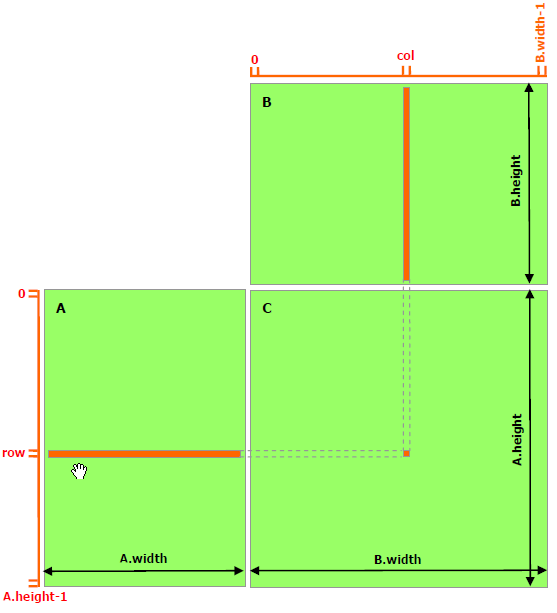
\includegraphics[width=0.8\textwidth, keepaspectratio]{images/ch1/CUDA-matrix-multiplication-without-shared-memory.png}
	\caption{Visualization of the execution of the kernel that does not use shared memory - shown in Listing~\ref{Listing:theory-CUDA-matrix-multiplication-without-shared-memory-example}. Taken from Nvidia's \emph{CUDA C++ Programming Guide} \cite{NVIDIAMay2022}.}
	\label{Figure:theory-CUDA-matrix-multiplication-without-shared-memory-example}
\end{figure}

\begin{lstlisting}[caption={Definition of the matrix multiplication kernel that uses global memory without shared memory. Each thread has a variable \code{Cvalue} stored in registers into which it calculates its specific \code{C(row, col)} matrix element. Taken from Nvidia's \emph{CUDA C++ Programming Guide} \cite{NVIDIAMay2022}.},label={Listing:theory-CUDA-matrix-multiplication-without-shared-memory-example}]
// Matrix multiplication kernel called by MatMul()
__global__ void MatMulKernel( Matrix A, Matrix B, Matrix C )
{
	// Each thread computes one element of C by accumulating results into Cvalue
	float Cvalue = 0;
	int row = blockIdx.y * blockDim.y + threadIdx.y;
	int col = blockIdx.x * blockDim.x + threadIdx.x;
	for( int i = 0; i < A.width; ++i ) {
		Cvalue += A.values[row * A.width + i] * B.values[i * B.width + col];
	}

	C.values[row * C.width + col] = Cvalue;
}
\end{lstlisting}

As can be seen in Listing~\ref{Listing:theory-CUDA-matrix-multiplication-without-shared-memory-example}, each thread performs \code{A.width + B.height} reads from global memory when calculating its \code{Cvalue}. Since CUDA threads are executed simultaneously in a warp of 32 threads, the memory access to global memory should be coalesced for the threads within each warp. Nevertheless, this kernel is suboptimal as accessing global memory is considered suboptimal when avoidable.
\par At the end of the introduction to Section~\ref{Subsection:matrix-multiplication}, it was mentioned that in order to eliminate the "matrix dimensions being multiples of \code{BLOCK\_SIZE}" requirement, the kernel would need to include a boundary condition. In this example, the condition would be simply to allocate an extra column and row of thread blocks to the grid. This would mean that the last row and column of blocks would overlap the dimensions of the matrix. Then, the kernel would be terminated for threads that are outside the matrix dimensions, i.e. if either \code{row} is greater than \code{A.height} or \code{col} is greater than \code{B.width}. However, it is noteworthy that this will result in thread divergence, even though in this instance it will not have a large impact on overall performance as one of the execution paths would be a simple \code{return} statement.

\subsubsection{Example with Shared Memory}\label{Subsubsection:theory-CUDA-matrix-multiplication-example-with-shared-memory}
The second example uses both global and shared memory. Similarly to the approach without using shared memory, each thread is responsible for calculating a single element of the resulting \code{C} matrix. However, in this example, each thread is also responsible for loading elements of matrices \code{A} and \code{B} from global memory into shared memory. Thus, shared memory is the primary means of obtaining elements for calculations. Overall, the calculation is changed from each thread calculating its individual element to a block of threads iterating over submatrices of \code{A} and \code{B}.
\par In order to make use of shared memory, matrix \code{C} is divided into submatrices of \code{BLOCK\_SIZE x BLOCK\_SIZE} elements ($ \mathbb{C}_{sub} $). Then, each submatrix $ \mathbb{C}_{sub} $ is computed by a single thread block; each thread within a thread block is responsible for the computation of an element in $ \mathbb{C}_{sub} $. In the previous approach, each thread performed element-wise multiplication of a row and a column to form a resulting element of matrix \code{C} - effectively a multiplication of an \code{1xn} and \code{nx1} matrix. The approach with shared memory expands this concept to blocks. In other words, the submatrix $ \mathbb{C}_{sub} $ is a result of multiplying two rectangular submatrices of \code{A} and \code{B} (illustrated in Figure~\ref{Figure:theory-CUDA-matrix-multiplication-with-shared-memory-example}) - denoted $ \mathbb{A}_{rect} $ and $ \mathbb{B}_{rect} $ for the purpose of this explanation:

\begin{enumerate}
	\item $ \mathbb{A}_{rect} $ is a \code{BLOCK\_SIZE x A.width} submatrix of \code{A} that has the same row indices as $ \mathbb{C}_{sub} $.
	\item $ \mathbb{B}_{rect} $ is a \code{B.height x BLOCK\_SIZE} submatrix of \code{B} that has the same column indices as $ \mathbb{C}_{sub} $.
\end{enumerate}

\begin{figure}[ht!]
	\centering
	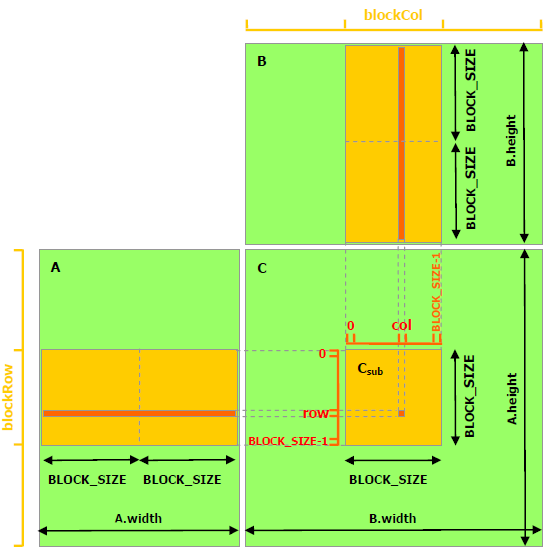
\includegraphics[width=0.8\textwidth, keepaspectratio]{images/ch1/CUDA-matrix-multiplication-with-shared-memory.png}
	\caption{Visualization of the execution of the kernel that uses shared memory - shown in Listing~\ref{Listing:theory-CUDA-matrix-multiplication-with-shared-memory-example}. Taken from Nvidia's \emph{CUDA C++ Programming Guide} \cite{NVIDIAMay2022}.}
	\label{Figure:theory-CUDA-matrix-multiplication-with-shared-memory-example}
\end{figure}

The rectangular submatrices $ \mathbb{A}_{rect} $ and $ \mathbb{B}_{rect} $ are split into \code{BLOCK\_SIZE x BLOCK\_SIZE} submatrices $ \mathbb{A}_{sub} $ and $ \mathbb{B}_{sub} $. A thread block will begin its computation by multiplying the leftmost $ \mathbb{A}_{sub} $ with the uppermost $ \mathbb{B}_{sub} $, then it will move to the next $ \mathbb{A}_{sub} $ on the right and to the next $ B_{sub} $ below. After every iteration, each thread appends its partial sum to the \code{Cvalue} variable that it is responsible for in the $ \mathbb{C}_{sub} $ submatrix. The computation of $ \mathbb{C}_{sub} $ is finished once the thread block reaches and multiplies the rightmost $ \mathbb{A}_{sub} $ and the lowermost $ \mathbb{B}_{sub} $ submatrix. \\
The reasoning behind splitting $ \mathbb{A}_{rect} $ and $ \mathbb{B}_{rect} $ into multiple $ \mathbb{A}_{sub} $ and $ \mathbb{B}_{sub} $ respectively stems from the use of shared memory in every iteration for a particular block:

\begin{enumerate}
	\item All threads of the block load $ \mathbb{A}_{sub} $ and $ \mathbb{B}_{sub} $ from global memory to a two-dimensional array residing in the block's shared memory.
	\item Each thread of the block performs its computation, i.e. it multiplies row \code{row\_id} from\space $ \mathbb{A}_{sub} $ with column \code{col\_id} from$ \mathbb{B}_{sub} $ and sums the resulting values (\code{row\_id} and \code{col\_id} are the thread's IDs).
	\item Each thread stores the temporary result to its local variable \code{Cvalue} stored in its registers.
	\item If there still is a $ \mathbb{A}_{sub} $ to the right and a $ \mathbb{B}_{sub} $ below, then, all threads of the block move to them and continue to step 1.
	\item Otherwise, the computation is finished and all threads store their local variable \code{Cvalue} to the element that they're responsible  in $ \mathbb{C}_{sub} $ that resides in global memory.
\end{enumerate}

The visualization of this approach is shown in Figure~\ref{Figure:theory-CUDA-matrix-multiplication-with-shared-memory-example} and the kernel is presented in Listing~\ref{Listing:theory-CUDA-matrix-multiplication-with-shared-memory-example}.

\begin{lstlisting}[caption={Definition of the matrix multiplication kernel that uses both global memory with shared memory. The \code{GetSubMatrix(mtx, row, col)} is a function returns a \code{BLOCK\_SIZE x BLOCK\_SIZE} submatrix of a matrix that is located \code{col} submatrices to the right and \code{row} submatrices down from the upper-left corner of a the specified \code{Matrix}. The \code{GetElement(sub\_mtx, row, col, val)} function returns the element found at a matrices \code{row} and \code{col} indices. Taken from Nvidia's \emph{CUDA C++ Programming Guide} \cite{NVIDIAMay2022}.},label={Listing:theory-CUDA-matrix-multiplication-with-shared-memory-example}]
// Matrix multiplication kernel called by MatMul()
__global__ void MatMulKernel( Matrix A, Matrix B, Matrix C )
{
	// Block row and column - indices of the submatrices within A and B respectively
	int blockRow = blockIdx.y;
	int blockCol = blockIdx.x;
	
	// Each thread block computes one submatrix Csub of C
	Matrix Csub = GetSubMatrix( C, blockRow, blockCol );
	
	// Each thread computes one element of Csub by accumulating results into Cvalue
	float Cvalue = 0;
	
	// Thread row and column within Csub
	int row = threadIdx.y;
	int col = threadIdx.x;
	
	// Loop over all the submatrices of A and B that are required to compute Csub by multiplying each pair of submatrices together and accumulate the results
	for( int i = 0; i < ( A.width / BLOCK_SIZE ); ++i ) {
		
		// Get submatrix Asub of A
		Matrix Asub = GetSubMatrix( A, blockRow, i );
		
		// Get submatrix Bsub of B
		Matrix Bsub = GetSubMatrix( B, i, blockCol );
		
		// Shared memory used to store Asub and Bsub respectively
		__shared__ float As[BLOCK_SIZE][BLOCK_SIZE];
		__shared__ float Bs[BLOCK_SIZE][BLOCK_SIZE];
		
		// Load Asub and Bsub from device memory to shared memory
		// Each thread loads one element of each submatrix
		As[row][col] = GetElement( Asub, row, col );
		Bs[row][col] = GetElement( Bsub, row, col );
		
		// Synchronize to make sure the submatrices are loaded before starting the computation
		__syncthreads();
		// Multiply Asub and Bsub together
		for( int k = 0; k < BLOCK_SIZE; ++k ) {
			Cvalue += As[row][k] * Bs[k][col];
		}
		
		// Synchronize to make sure that the preceding computation is done before loading two new submatrices of A and B in the next iteration
		__syncthreads();
	}
	
	// Write Csub to device memory - each thread writes one element
	SetElement( Csub, row, col, Cvalue );
}
\end{lstlisting}

Unlike the previous example, the code shown in Listing~\ref{Listing:theory-CUDA-matrix-multiplication-with-shared-memory-example} has less accesses to global memory which leads to an performance improvement as detailed later in the \textit{\nameref{Subsubsection:matrix-multiplication-comparison-of-examples}} part of Section~\ref{Subsubsection:matrix-multiplication-comparison-of-examples}. Concretely, in the kernel above, each thread performs only \code{A.width/BLOCK\_SIZE + B.height/BLOCK\_SIZE} reads from global memory when loading submatrices $ \mathbb{A}_{sub} $ and $ \mathbb{B}_{sub} $ into shared memory. This means that all threads will perform \code{BLOCK\_SIZE} times less accesses to global memory and \code{A.width + B.height} accesses to shared memory instead. Equivalently to the example before, the access to global memory is coalesced. Thus, by Nvidia's recommendations, this kernel can be considered being close to optimal.

\par In order to eliminate the "matrix dimensions being multiples of \code{BLOCK\_SIZE}" requirement, the kernel would need to include a boundary condition. In the earlier approach it was a matter of allocating extra blocks and terminating the kernel for threads that would reach out of matrix bounds. However, for this approach - with shared memory - that method would result in incorrect results as the threads that would reach out of bounds for one matrix read elements into shared memory from the other matrix. Thus, the boundary condition is split into:

\begin{enumerate}
	\item If the thread would reach out of bounds of a particular matrix, load the edge element, i.e. the last element of the row/col before the thread would reach out of bounds. This condition would be used when the elements are being loaded from global into shared memory.
	\item Then let the computation continue as normal - to avoid thread divergence of threads.
	\item Once the computation si done, terminate the threads that would reach out of bounds of matrix \code{C} before they write their results to global memory.
\end{enumerate}

This solution ensures correct results and avoids a case of thread divergence in the main loop which would occur multiple times during the computation. However, the thread divergence will still occur when deciding which value to load from global memory and when terminating the kernel for some threads. Nevertheless, similarly to the previous approach, in this instance thread divergence will not have a large impact on overall performance as one of the execution paths would be a simple assignment operation in the first condition and a \code{return} statement in the second condition.

\subsubsection{Comparison of Both Examples}\label{Subsubsection:matrix-multiplication-comparison-of-examples}
In order to show the performance difference, benchmarks for both examples using single precision were run on a set of matrices with varying dimensions - from 160 by 160 to 16,000 by 16,000. The hardware and software specifications of the machine used for the benchmarks can be found in Table~\ref{Table:theory-CUDA-matrix-multiplication-benchmark-system}. The code used for the comparison was taken from Nvidia's GitHub repository  \textit{CUDA Samples}\footnote{CUDA Samples GitHub repository URL: \url{https://github.com/NVIDIA/cuda-samples}}, specifically from \code{cuda-samples/Samples/0\_Introduction/matrixMul/}.

\begin{table}[h]
	\centering
	\begin{tabular}{|l|l|}
		\hline
		CPU              & Ryzen 9 5900x @ 3.7 GHz (12 cores, 24 threads) \\
		RAM              & 32GB RAM \\
		GPU              & Nvidia GeForce GTX 1070 8GB GDDR5 (256.3 GByte/s)\\
		Operating System & Ubuntu 20.04.4 LTS (Focal Fossa) \\
		Compiler         & GCC 8.4.0 \\
		CUDA             & CUDA 11.5 \\ \hline
	\end{tabular}
	\caption{Specifications of the platform that the matrix multiplication benchmarks were run on.}
	\label{Table:theory-CUDA-matrix-multiplication-benchmark-system}
\end{table}

The operation measured during the benchmark was only the multiplication of matrices
$$ \mathbb{C} = \mathbb{A} \cdot \mathbb{B} $$
In other words, allocation and copying of the matrices was not included in the measurement. Furthermore, the operation was looped 10 times - the measured FLOPS and run times were averaged from the 10 recorded loops. The values in Matrix $ \mathbb{A} $ were all set to 1 and to 0.1 in matrix $ \mathbb{B} $. The benchmark results in FLOPS can be found in Figure~\ref{Figure:theory-CUDA-matrix-multiplication-benchmark-results-flops} and Table~\ref{Table:theory-CUDA-matrix-multiplication-benchmark-results-msec} shows the results in milliseconds.

\begin{figure}
	\centering
	\tikzset{mark options={mark size=2.5, line width=1pt}}
	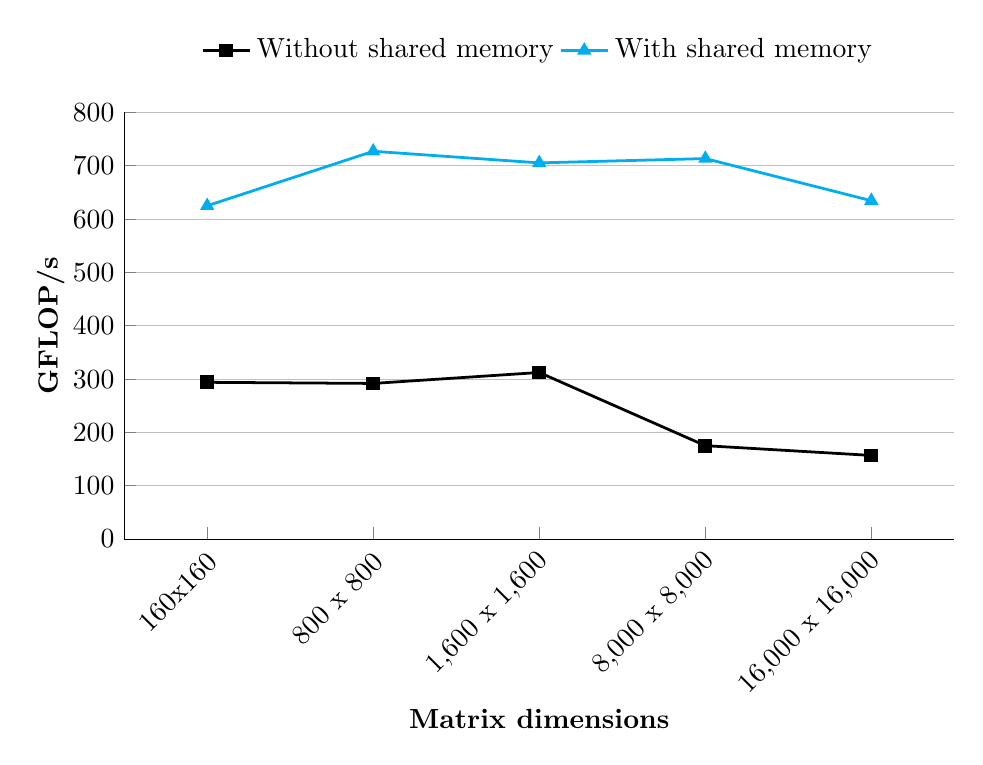
\begin{tikzpicture}
		\begin{axis}
			[
			,width=\textwidth
			,height=7cm
			,axis x line*=bottom
			,axis y line*=left
			,xlabel=\textbf{Matrix dimensions}
			,x label style={at={(axis description cs:0.5,-0.375)},anchor=north,font=\normalsize}
			,ylabel=\textbf{GFLOP/s}
			,y label style={at={(axis description cs:-0.06,.5)},rotate=0,anchor=south,font=\normalsize}
			,xmin=0.5, xmax=5.5
			,ymin=0, ymax=800
			,xtick=data,
			,xtick pos=left
			,ytick={0,100,200,300,400,500,600,700,800}
			,ytick pos=left
			,xticklabels={160x160,800 x 800,{1,600 x 1,600},{8,000 x 8,000},{16,000 x 16,000}}
			,x tick label style={rotate=45,anchor=east,yshift=-6pt,align=right,font=\normalsize}
			,y tick label style={font=\normalsize}
			,ymajorgrids
			,scatter/classes={
				shared-mem={mark=square*,blue},
				no-shared-mem={mark=triangle*,black}
			}
			,legend style={at={(0.5,1.2)},anchor=north,font=\normalsize,cells={anchor=east}, legend columns=-1,draw=none}
			]
			\addplot[black,line width=1pt,mark=square*,mark options={mark size=2}] coordinates {
				(1, 293.96) [no-shared-mem]
				(2, 291.84) [no-shared-mem]
				(3, 312.38) [no-shared-mem]
				(4, 175.16) [no-shared-mem]
				(5, 156.85) [no-shared-mem]
			};
			\addplot[cyan,line width=1pt,mark=triangle*] coordinates {
				(1, 625.00) [shared-mem]
				(2, 727.18) [shared-mem]
				(3, 705.41) [shared-mem]
				(4, 713.48) [shared-mem]
				(5, 634.50) [shared-mem]
			};
			\legend{Without shared memory, With shared memory}
		\end{axis}
	\end{tikzpicture}
	\caption{Matrix multiplication results of matrices with varying dimensions; matrices are filled with 1 element. The values - presented in GFlop/s - are averages from 10 loops of the operation.}
	\label{Figure:theory-CUDA-matrix-multiplication-benchmark-results-flops}
\end{figure}

\begin{table}[ht!]
	\centering
	\renewcommand{\arraystretch}{1.5}
	\begin{tabular}{ |c|r|r| } 
		\hline
		\multicolumn{1}{|c|}{Matrix dimensions} & \multicolumn{1}{c|}{Without shared memory} & \multicolumn{1}{c|}{With shared memory} \\
		\hline
		160 x 160 & 0.028 & 0.013 \\
		\hline
		800 x 800 & 3.509 & 1.408 \\
		\hline
		1,600 x 1,600 & 26.224 & 11.613 \\
		\hline
		8,000 x 8,000 & 5,846.247 & 1,435.221 \\
		\hline
		16,000 x 16,000 & 52,226.867 & 12,910.967 \\
		\hline
	\end{tabular}
	\caption{Matrix multiplication execution times (in milliseconds) of matrices with varying dimensions; matrices are filled with 1 element. The values are averages from 10 loops of the operation.}
	\label{Table:theory-CUDA-matrix-multiplication-benchmark-results-msec}
\end{table}

As can be seen in Figure~\ref{Figure:theory-CUDA-matrix-multiplication-benchmark-results-flops} and Table~\ref{Table:theory-CUDA-matrix-multiplication-benchmark-results-msec}, the approach that utilizes shared memory achieved between 2-4 times the number of GFLOPs per second and similarly faster execution times compared to the approach that does not use shared memory and instead relies only on global memory. Additionally, the difference seems to be increasing with growing matrix dimensions, however, this statement has not been verified for dimensions greater than 16,000 by 16,000.



\section{LU Decomposition}\label{Section:theory-LU-decomposition}
It can be argued that, in recent years, computational systems and software layers allowing developers to use them to their full potential have developed significantly - Nvidia GPUs and CUDA. Subsequently, many novel uses have been found for such powerful computing systems, especially in areas that require results to be available quickly on demand. An example of such an area is solving systems of linear equations. Being one of the fundamental parts of numerical linear algebra, the requirement for their solution arises not only in computer science, but also in physics, engineering, chemistry, etc. \\
While there are many different methods capable of solving a system comprising of more than one linear equation, in this project, Lower-Upper (LU) decomposition will be detailed. \\
In order to show how LU decomposition can be used to solve a simple system of linear equations an example will be presented. 
\par \textbf{First}, it is necessary to introduce the system. For the purpose of the explanation, let the coefficients of the following system of linear equations:

\begin{align}
	a_{11}x_1 + a_{12}x_2 + a_{13}x_{3}&= \,b_1 \nonumber\,, \\ 
	a_{21}x_1 + a_{22}x_2 + a_{23}x_{3}&= \,b_2 \label{Equation:theory-LU-decomposition-system-linear-equations}\,, \\
	a_{31}x_1 + a_{32}x_2 + a_{33}x_{3}&= \,b_3 \nonumber\,,
\end{align}

be rewritten into the matrix form

\begin{equation}\label{Equation:theory-LU-decomposition-system-linear-equations-matrix-form-Axb}
	\mathbb{A}\textbf{x} = \textbf{b}\,,
\end{equation}

where

\begin{equation}
	\mathbb{A} = 
	\begin{bmatrix}
		a_{11} & a_{12} & a_{13} \\
		a_{21} & a_{22} & a_{23} \\
		a_{31} & a_{32} & a_{33}
	\end{bmatrix}
	,\quad
	\mathbf{x} = 
	\begin{bmatrix}
		x_{1} \\
		x_{2} \\
		x_{3}
	\end{bmatrix}
	,\quad
	\mathbf{b} = 
	\begin{bmatrix}
		b_{1} \\
		b_{2} \\
		b_{3}
	\end{bmatrix}.
\end{equation}

In order to be able to use LU decomposition, matrix $ \mathbb{A} $ must be a square matrix ($ n\times n $) that is also strongly regular. This requirement can be relaxed to only requiring regularity by properly ordering the rows and columns of the matrix using a permutation matrix $ \mathbb{P} $, however, such a procedure will not be present in this project, and therefore all coefficient matrices are required to be strongly regular.
\par \textbf{Second}, using a \textit{decomposition algorithm} the coefficient matrix $ \mathbb{A} $ is decomposed into the product of a lower triangular matrix $ \mathbb{L} $ and a upper triangular matrix $ \mathbb{U} $:

\begin{equation}
	\mathbb{A} = \mathbb{LU}\,,
\end{equation}

\begin{equation}
	\begin{bmatrix}
		a_{11} & a_{12} & a_{13} \\
		a_{21} & a_{22} & a_{23} \\
		a_{31} & a_{32} & a_{33}
	\end{bmatrix}
	=
	\begin{bmatrix}
		l_{11} & 0      & 0          \\
		l_{21} & l_{22} & 0          \\
		l_{31} & l_{32} & l_{33}
	\end{bmatrix}
	\begin{bmatrix}
		u_{11} & u_{12} & u_{13} \\
		0      & u_{22} & u_{23} \\
		0      & 0      & u_{33}
	\end{bmatrix}.
\end{equation}

Then, substituting Equation~\ref{Equation:theory-LU-decomposition-system-linear-equations-matrix-form-Axb} into Equation~\ref{Equation:theory-LU-decomposition-system-linear-equations-matrix-form-Axb} yields:

\begin{equation}\label{Equation:theory-LU-decomposition-system-linear-equations-matrix-form-LUxb}
	\mathbb{LU}\textbf{x} = \textbf{b}\,.
\end{equation}.

\par \textbf{Third}, the matrix form from Equation~\ref{Equation:theory-LU-decomposition-system-linear-equations-matrix-form-LUxb} is used to obtain the solution to the system of linear equations using forward and backward substitution:

\begin{enumerate}
	\item Solve the equation $ \mathbb{L}\textbf{y} = \textbf{b} $ (where only $ \textbf{y} $ is not known):
	\begin{equation}\label{Equation:theory-LU-decomposition-solving-Lyb}
		\begin{bmatrix}
			l_{11} & 0      & 0          \\
			l_{21} & l_{22} & 0          \\
			l_{31} & l_{32} & l_{33}
		\end{bmatrix}
		\begin{bmatrix}
			y_{1} \\
			y_{2} \\
			y_{3}
		\end{bmatrix}
		=
		\begin{bmatrix}
			b_{1} \\
			b_{2} \\
			b_{3}
		\end{bmatrix}.
	\end{equation}
	\item Solve the equation $ \mathbb{U}\textbf{x} = \textbf{y} $ (where only $ \textbf{x} $ is not known):
	\begin{equation}\label{Equation:theory-LU-decomposition-solving-Uxy}
		\begin{bmatrix}
			u_{11} & u_{12} & u_{13} \\
			0      & u_{22} & u_{23} \\
			0      & 0      & u_{33}
		\end{bmatrix}
		\begin{bmatrix}
			x_{1} \\
			x_{2} \\
			x_{3}
		\end{bmatrix}
		=
		\begin{bmatrix}
			y_{1} \\
			y_{2} \\
			y_{3}
		\end{bmatrix}.
	\end{equation}
\end{enumerate}

It is noteworthy that since the values on the right-hand side (vector $ \textbf{b} $) are only required in step 3 (equations~\ref{Equation:theory-LU-decomposition-solving-Lyb} and \ref{Equation:theory-LU-decomposition-solving-Uxy}), they are not required for the process of decomposition itself. Thus, if there is more than one right side in the system of linear equations, matrix $ \mathbb{A} $ needs to be decomposed into matrices $ \mathbb{L} $ and $ \mathbb{U} $ only once; the same principle is valid even if the right side is not known ahead of time. In other words, $ \mathbb{L} $ and $ \mathbb{U} $ can used to solve the system for different right-hand sides without the need for repeated decomposition. Additionally, this concept can be seen as an advantage for LU decomposition compared to Gaussian elimination as the latter requires the right-hand side to obtain the system's upper triangular matrix and subsequently use it for backward substitution. This concept is described, for example, by George Lindfield and John Penny in \emph{Numerical Methods: Linear Equations and Eigensystems} \cite{Lindfield2019}.

In summary, from the steps above, it can argued that the \textit{decomposition algorithm} mentioned in step 2 is one of the key components of the procedure and as such it will be the main topic of this project.

\subsection{Crout Method}\label{Subsection:theory-LU-decomposition-crout-method}
This section aims to explain in greater detail the decomposition algorithm mentioned above in step 2. There are many different procedures to decompose matrix $ \mathbb{A} $ into matrices $ \mathbb{L} $ and $ \mathbb{U} $ such that $ \mathbb{A} = \mathbb{LU} $. One such procedure, developed by Prescott Durand Croutis, is the \textit{Crout method} - sometimes also referred to as \textit{Crout matrix decomposition} or \textit{Crout factorization} \cite{Press2007}. \\
This method differs from similar procedures in that the resulting $ \mathbb{U} $ matrix is a unit upper triangular matrix, while $ \mathbb{L} $ remains to be a lower triangular matrix. A unit triangular matrix differs from a regular triangular matrix in that its main diagonal is comprised solely of ones. In other words, all elements on the main diagonal of $ \mathbb{U} $ are equal to 1 ($ u_{11} = u_{22} = u_{33} = 1 $):

\begin{equation}
	\begin{bmatrix}
		1      & u_{12} & u_{13} \\
		0      & 1      & u_{23} \\
		0      & 0      & 1
	\end{bmatrix}.
\end{equation}

\paragraph{Algorithm}
The Crout matrix decomposition algorithm is based on sequentially computing matrices $ \mathbb{L}_{n\times n} $ and $ \mathbb{U}_{n\times n} $ using elements from matrix $ \mathbb{A}_{n\times n} $. At the core of this computation are the following formulas and their conditions for $ l_{ij} $ and $ u_{ij} $:

\begin{align}
	l_{ij} &= a_{ij} - \sum_{k=1}^{j-1}l_{ik}u_{kj} 								  &\quad i \geq j\,, \label{Equation:theory-LU-decomposition-crout-method-lij} \\
	u_{ij} &= \frac{1}{l_{ii}} \left ( a_{ij} - \sum_{k=1}^{i-1}l_{ik}u_{kj} \right ) &\quad i < j\,, \\ \label{Equation:theory-LU-decomposition-crout-method-uij}
	u_{ij} &= 1 																	  &\quad i = j\,, \\
	i,j &\in \widehat{n} \nonumber\,.
\end{align}

Specifically, the algorithm first computes a column $ j $ in $ \mathbb{L} $ and then row $ j $ in $ \mathbb{U} $. This process repeats itself for $ j $ from 1 to $ n $. The pseudocode implementing the algorithm can be seen in Listing~\ref{Listing:theory-LU-decomposition-crout-method-pseudocode} and the visualization of the algorithm's advance is shown in Figure~\ref{Figure:theory-LU-decomposition-crout-method-visualisation}.

\begin{lstlisting}[caption={C++ pseudocode implementing Crout's matrix decomposition algorithm. It assumes that \code{A[n][n]} is a two-dimensional array that represents the invertible square coefficient matrix $ \mathbb{A} $; \code{L[n][n]} and \code{U[n][n]} are also two-dimensional arrays reprenting matrices $ \mathbb{L} $ and $ \mathbb{U} $ respectively. Furthermore, it is assumed that \code{L} and \code{U} are populated with zeros. Derived from \emph{Crout's LU Factorization} \cite{rqjYYJkSwERYYbSy}, \emph{Numerical recipes: the art of scientific computing} \cite{Press2007} and \emph{Crout matrix decomposition} \cite{TgtpOw7zCHo3ii0m}.},label={Listing:theory-LU-decomposition-crout-method-pseudocode}]
void crout_method( A, L, U )
{
	int i, j, k;
	double sum = 0;
	
	// Fill main diagonal of U with 1s
	for( i = 0; i < n; ++i ) {
		U[i][i] = 1;
	}	

	// Loop through the main diagonal
	for( j = 0; j < n; ++j ) {
		
		// Compute column j in L
		for( i = j; i < n; ++i ) {
			sum = 0;
			for( k = 0; k < j; ++k ) {
				sum += L[i][k] * U[k][j];
			}

			L[i][j] = A[i][j] - sum;
		}
		
		// Compute row j in U
		for( i = j; i < n; ++i ) {
			sum = 0;
			for( k = 0; k < j; ++k ) {
				sum = sum + L[j][k] * U[k][i];
			}

			if( L[j][j] == 0 ) {
				printf( "det(L) close to 0!\n Can't divide by 0...\n" );
				exit( EXIT_FAILURE );
			}

			U[j][i] = ( A[j][i] - sum ) / L[j][j];
		}
	}
}
\end{lstlisting}

\begin{figure}[ht!]
	\centering
	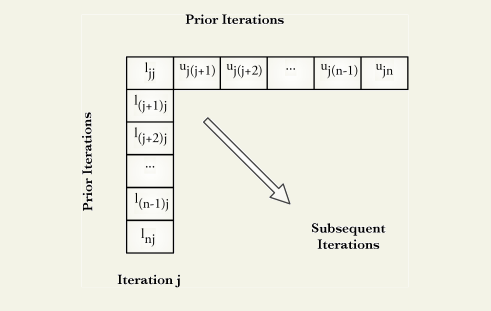
\includegraphics[width=0.8\textwidth, keepaspectratio]{images/ch1/LU_decomposition_crout_method_visualization.png}
	\caption{Sequence of computations of the Crout method. First, column $ j $ in $ \mathbb{L} $ is computed and then row $ j $ of $ \mathbb{U} $. Taken from Vismor's \emph{Crout's LU Factorization} \cite{rqjYYJkSwERYYbSy}.}
	\label{Figure:theory-LU-decomposition-crout-method-visualisation}
\end{figure}

\subsection{Numerical Method}\label{Subsection:theory-LU-decomposition-numerical-method}
When solving systems of linear equations there are two main groups of methods:

\begin{enumerate}
	\item Direct methods - theoretically, the exact solution will be obtained after a finite amount of steps (e.g. Crout method).
	\item Iterative methods - theoretically, these methods converge to the solution, however, the exact solution is not guaranteed to be found (numerical methods).
\end{enumerate}

The Crout method as described in Section~\ref{Subsection:theory-LU-decomposition-crout-method} is a direct method, meaning that it provides an exact solution. Furthermore, it is strictly sequential, meaning that there is seemingly no room for parallelization. \\
However, Hartwig Anzt et al. in their paper \emph{ParILUT - A Parallel Threshold ILU for GPUs} \cite{Anzt2019} describe different approaches to generating incomplete factorizations. An example of such a group of approaches is referred to as \textit{ParILU algorithms} which are distinct in the fact that they abandon the methodology akin to Gaussian elimination. Rather, these methods use "\textit{fixed-point iterations to approximate the incomplete factors on a pre-defined sparsity pattern}" - iterative methods. The authors in the paper explain the methods belonging to this group as algorithms that do not take every nonzero into account. \\
However, for the purpose of this paper, it was decided to derail from this principle - exclude any sparsity pattern conditions - and focus purely on the iterative aspect of the methodology. In other words, use the fixed-point iterating algorithm that - according to the authors - converges to a sufficiently approximate solution of $ \mathbb{A} = \mathbb{LU} $ without taking into account sparsity patterns. \\
Specifically, the algorithm is as follows:

\begin{enumerate}
	\item Provide an initial guess (estimate) of matrices $ \mathbb{L}^0 $ and $ \mathbb{U}^0 $. For example, using $ \mathbb{A} $:
		\begin{align}
			l_{ij}^{0} &= a_{ij} \quad &i < j \nonumber\,, \\
			u_{ij}^{0} &= a_{ij} \quad &i > j \nonumber\,, \\
			u_{ij}^{0} &= 1 \quad      &i = j \nonumber\,.
		\end{align}
	\item Using the formulas in Equations~\ref{Equation:theory-LU-decomposition-crout-method-lij} and \ref{Equation:theory-LU-decomposition-crout-method-lij} calculate the next iteration of $ \mathbb{L}^{t} $ and $ \mathbb{U}^{t} $ (where $ t \in \widehat{\mathbb{N}}_0 $ denotes the iteration): $ \mathbb{L}^{t+1} $ and $ \mathbb{U}^{t+1} $
		\begin{align}
			l_{ij}^{t+1} &= a_{ij} - \sum_{k=1}^{j-1}l_{ik}^{t}u_{kj}^{t} 								   		&\quad i \geq j \nonumber\,, \\
			u_{ij}^{t+1} &= \frac{1}{l_{ii}^{t}} \left ( a_{ij} - \sum_{k=1}^{i-1}l_{ik}^{t}u_{kj}^{t} \right ) &\quad i < j    \nonumber\,. 
		\end{align}
	\item If either $ \left | \mathbb{L}^{t+1} - \mathbb{L}^{t} \right | $ or $ \left | \mathbb{U}^{t+1} - \mathbb{U}^{t} \right | $ is greater than some tolerance, e.g. $ 0.001 $, then go back to step 2.
	\item If both differences are smaller than the tolerance, then the algorithm has iteratively converged to an approximate solution of $ \mathbb{A} = \mathbb{LU} $.
\end{enumerate}

On one hand, the number of iterations it takes the algorithm to converge to a solution is not possible to accurately predict and therefore could lead to poor performance if performed sequentially. On the other hand, since $ \mathbb{L}^{t+1} $ and $ \mathbb{U}^{t+1} $ are calculated independently, the operation can be run in parallel. \\
Another noteworthy, but unverified, aspect of this method's convergent nature is related to rounding errors. Specifically, since Crout's method is direct, it can be theorized that rounding errors may result in it providing less accurate results compared to its numerical modification. This thought stems from the fact that the numerical method converges and thus - under specific convergence rules - may arrive at a more accurate solution. However, this is purely a hypothesis and remains to be verified. \\
Joining together the highly parallel nature of CUDA-enabled Nvidia GPUs and such a heavily parallelizable algorithm is the main focus of this project and will be detailed further in the following chapters.

\chapter{Implementation \TO}\label{Chapter:implementation-introduction}
This chapter will present the implementation of the \textit{Decomposition} project that was built around the algorithms described in Sections~\ref{Subsection:LU-decomposition-crout-method} and \ref{Subsection:LU-decomposition-numerical-method}. First, the \textit{TNL} library\footnote{TNL Library GitLab repository URL: \url{https://gitlab.com/tnl-project/tnl}} will be introduced briefly as it contains a structure that was paramount to the implementation of this project. Then, the description of the \textit{Decomposition} project itself will follow. Finally, the last section will present how the iterative algorithm, mentioned in Section~\ref{Subsection:LU-decomposition-numerical-method}, was fine-tuned for optimal performance using CUDA.

\section{TNL Library \TO}\label{Section:implementation-tnl-library}
The Template Numerical Library (TNL) is a collaborative, open-source project licensed under the MIT license. It aims to use modern programming paradigms combined with the computational power of parallel architectures to provide highly performant numerical solvers and simulations. In terms of parallel architectures, TNL supports both multi-core CPUs (using OpenMP\footnote{OpenMP website URL: \url{https://www.openmp.org/}}) and GPUs (as of July 2022 only CUDA-enabled Nvidia GPUs with compute capability 9.0 or higher \cite{Ednu6dyrkWKz1Bv2}). As TNL is written in C++ (with the exception of some helping Python/Bash scripts) it is designed to benefit from C++ templates and the advantages they bring. For example, the use of template specializations allows for minimal run-time overhead which makes execution of architecture-dependent code simple and fast \cite{Oberhuber20210210}. Further up-to-date information regarding TNL can be found on the project's website\footnote{TNL project website URL: \url{https://tnl-project.org/}}. \\
While TNL contains, among others, many different data structures. For the purpose of this project only the one used during development will be introduced.

\paragraph{Dense matrix}\label{Paragraph:implementation-tnl-library-dense-matrix}
As mentioned at the end of Section~\ref{Subsection:LU-decomposition-numerical-method}, the goal of this project is to combine the parallel nature of CUDA-enabled Nvidia GPUs and the heavily parallelizable algorithm described in the same section (labeled as \textit{Iterative Crout method} for the purpose of this project). \\
Therefore, in order to store all matrices involved in the computation, an efficient, robust and intuitive data structure was required. While in terms of matrices TNL mainly revolves around sparse implementations (i.e. efficiently storing and performing operations with matrices that have more zero than non-zero elements), it also possesses the opposite: \textit{dense matrices}. As the name suggest, dense matrices are matrix structures densely populated with elements. In other words, a dense matrix stores every single element, regardless of its value (zeros and non-zeros are stored). In TNL, the class representing the dense matrix data structure is called \code{DenseMatrix} and it is located in the \code{TNL::Matrices} namespace. Similarly to the majority of classes representing matrices in TNL, it inherits from the \code{Matrix} class; the visualization of inheritance can be found in Figure~\ref{Figure:implementation-tnl-library-dense-matrix}.

\begin{figure}[h!]
	\centering
	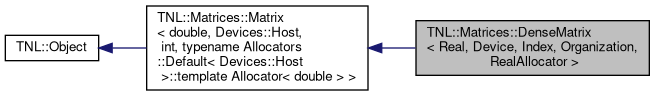
\includegraphics[width=\textwidth, keepaspectratio]{images/ch2/tnl_matrices_dense_matrix-inheritance.png}
	\caption{Inheritance diagram for the \code{TNL::Matrices::DenseMatrix} class. Taken from the \emph{Template Numerical Library Documentation} \cite{Ednu6dyrkWKz1Bv2}.}
	\label{Figure:implementation-tnl-library-dense-matrix}
\end{figure}

In the diagram shown in Figure~\ref{Figure:implementation-tnl-library-dense-matrix} the \code{DenseMatrix} class contains the following template parameters \cite{Ednu6dyrkWKz1Bv2}:

\begin{itemize}
	\item \code{Real} - Datatype of the matrix's elements, for example, \code{float} or \code{double} (default).
	\item \code{Device} - Type of device that the matrix structure is stored on. Its value can be either \code{TNL::Devices:Host} (default) or \code{TNL::Devices::Cuda}. The former indicates that the structure is stored in host memory, whereas the latter indicates that the data is stored in device memory. Furthermore, this parameter dictates which of the class's methods can be called and what device-dependent code should be executed.
	\item \code{Index} - Datatype of the matrix's index, for example, \code{short}, \code{int} (default), or \code{long}.
	\item \code{Organization} - Type of matrix element ordering. It can be either \code{RowMajorOrder} or \code{ColumnMajorOrder}. The former indicates that the elements of the matrix are stored in row-major order in a \code{DenseMatrix} instance's 1D array \code{values}, whereas the latter dictates that the elements are stored in the array in a column-major order. Implicitly, row-major order is used when the structure is allocated on the host and column-major order if it is allocated on the device.
	\item \code{RealAllocator} - Allocator for the matrix elements.
\end{itemize}

The \code{DenseMatrix} class contains an assortment of methods with varying functionalities - from the initialization of an entire matrix via arrays to per-element lambda functions and CUDA-tailored algorithms. In terms of this project, the most used methods were those that set and get elements, which can be done by using \code{setElement()} and \code{getElement()} respectively. Alternatively, for setting and getting elements, \code{DenseMatrix} possesses the overloaded operator: \code{operator()}, which allows the developer to write cleaner code that conveys its purpose more clearly. From the perspective of performance, both approaches are congruous as they take the same arguments and compute the index of the element in the instance's 1D array. Nonetheless, there is a difference between the two approaches: \code{operator()} has the \code{\_\_cuda\_callable\_\_} prefix, which specifies that it can be called from both host functions and CUDA kernels. However, this prefix comes with certain caveats:

\begin{itemize}
	\item Data allocated on the host can only be accessed by \code{operator()} from host functions.
	\item Data allocated on the device can only be accessed by \code{operator()} from the device, specifically, from CUDA kernels. For example, if an instance of \code{DenseMatrix} has \code{Device} set to \code{TNL::Devices::Cuda} and \code{operator()} would be used to access data from a host function, then the program would fail.
\end{itemize}

The limitations above are not present for the other approach (\code{setElement()} and \code{getElement()}). In other words, both \code{setElement()} and \code{getElement()} can be used from host functions and CUDA kernels, irrespective of where the \code{DenseMatrix} instance is allocated. However, this convenience has a pitfall: accessing data stored on the other device type. For example, let an instance of \code{DenseMatrix} be stored in device memory. Then, if it is accessed from a host function using \code{getElement()}, the procedure will be slow and only the value of the element will be returned. Listing~\ref{Listing:implementation-dense-matrix-getters-setters} shows an example of both approaches - including the caveats and pitfalls.

\begin{lstlisting}[caption={Code example showing the use of \code{setElement()}, and \code{operator()}; \code{getElement()} and getting a matrix element using \code{operator()} would be done similarly. The example requires the TNL library to already be installed. As mentioned in the code, the \code{setElements()} function will run correctly when evoked using the \code{TNL::Devices::Host} template parameter. However, if the \code{DenseMatrix} instance is allocated on the device, then the first setting of elements (using \code{setElement()}) will be slow due to the data transfer between the host and the device - each call will mean a unique data transfer. Furthermore, the second setting of elements (using \code{operator()}) will fail as \code{operator()} will be called from a host function on a \code{DenseMatrix} instance allocated on the device. For the second setter to work, it would need to be called from within a kernel. Taken from section \code{Tutorials/Matrices/DenseMatrices} in the \emph{Template Numerical Library Documentation} \cite{Ednu6dyrkWKz1Bv2}.},label={Listing:implementation-dense-matrix-getters-setters}]
#include <iostream>
#include <TNL/Matrices/DenseMatrix.h>
#include <TNL/Devices/Host.h>

template< typename Device >
void setElements()
{
	// Create an instance of 5x5 DenseMatrix
	TNL::Matrices::DenseMatrix< double, Device > matrix( 5, 5 );
	
	// Set elements of the main diagonal using setElement()
	for( int i = 0; i < 5; ++i ) {
		matrix.setElement( i, i, i );
	}

	// Increment elements of the main diagonal using operator()
	for( int i = 0; i < 5; ++i ) {
		matrix( i, i ) += i;
	}
}

int main( int argc, char* argv[] )
{
	// This example will run without any problems
	std::cout << "Set elements on host:" << std::endl;
	setElements< TNL::Devices::Host >();
	
#ifdef HAVE_CUDA
	// This example will fail on the second setting of elements
	std::cout << "Set elements on CUDA device:" << std::endl;
	setElements< TNL::Devices::Cuda >();
#endif
}
\end{lstlisting}

More detailed information on the structure's implementation can be found under \code{Namespaces/TNL/Matrices/DenseMatrix} in \emph{Template Numerical Library Documentation} \cite{Ednu6dyrkWKz1Bv2} and further examples of usage can be found under \code{Tutorials/Matrices/DenseMatrices}.



\section{Decomposition Project \TO}\label{Section:implementation-decomposition-project}
Even though the \code{DenseMatrix} class from TNL is used in the Decomposition project - and a select few solvers are already implemented in TNL - it was decided to create a separate repository\footnote{\label{Footnote:decomposition-project-gitlab-url}Decomposition GitLab repository URL: \url{https://mmg-gitlab.fjfi.cvut.cz/gitlab/tnl/lu-decomposition}} in GitLab solely for this rendition of decomposition. Since the project is continually under development it is only available internally,
i.e. to users belonging to the TNL group on the Mathematical Modelling Group's\footnote{MMG main page URL: \url{https://geraldine.fjfi.cvut.cz/mmg/index.php}} GitLab page\footnote{TNL GitLab group URL: \url{https://mmg-gitlab.fjfi.cvut.cz/gitlab/tnl}}. \\
Although development was done outside of TNL, its structuring and building processes were adopted with minor changes to allow for easier familiarization and to keep the option of incorporating the Decomposition project into TNL open for the future. The compilation/installation of the project is done using the \code{install} Bash script that was adopted from TNL. The script itself serves as a wrapper for the \code{build} script that takes several building arguments, for example, the mandatory target parameter allows the user to choose to build one of the following:

\begin{itemize}
	\item \code{all} - compile the entire project including all other targets and the algorithm implementations.
	\item \code{benchmark} - compile the benchmark only.
	\item \code{tests} - compile the unit tests only.
\end{itemize}

Additionally, the \code{build} script provides optional parameters that can aid in compilation, for example:
\begin{itemize}
	\item \code{---install} - enables installation of the Decomposition project files into \code{\$HOME/.local/include}.
	\item \code{---cmake} - allows the user to supply the path to the CMake that is to be used for compilation.
	\item \code{---with-cuda-arch} - allows the user to specify the CUDA compute capability version to compile the project with. While there is an auto-detect feature for this parameter, the manual setting can be indispensable in some situations, for example, when running the benchmark on a computational cluster the compilation is usually done beforehand on a node that is not guaranteed to have a CUDA-enabled GPU. 
\end{itemize}

The full list of compilation options (\code{build} script usage) can be found in Attachment~\ref{Attachment:decomposition-project-build-script-parameters}. \\
The \code{build} script then calls CMake\footnote{CMake website URL: \url{https://cmake.org/}} which subsequently takes care of the build process using instructions from \code{CMakeLists.txt} files interspersed throughout the project. \\
The Decomposition project was written in \textit{C++} which was extended by \textit{CUDA} (GPU programming) and \textit{GoogleTest}\footnote{\label{Footnote:google-test}GoogleTest GitHub repository URL: \url{https://github.com/google/googletest}} (unit testing - approach adopted from TNL's matrix unit tests). Additionally, \textit{Python}\footnote{Python website URL: \url{https://www.python.org/}} and \textit{Bash}\footnote{Bash website URL: \url{https://www.gnu.org/software/bash/}} were used when adopting scripts from TNL, for example, a python script that creates tables and graphs in HTML from json files generated by the benchmark. \\
In this section, each part of the project's structure will be briefly described. First, unit tests will be detailed followed by the implementation of the Crout method (introduced in Section~\ref{Subsection:LU-decomposition-crout-method}), along with the Iterative Crout method (introduced in Section~\ref{Subsection:LU-decomposition-numerical-method}). Finally, the last part focuses on the benchmark implementation that aims to put into perspective the performance differences between the direct and iterative approach. \\
The ordering of topics follows the development process which was inspired by Test-driven development\footnote{Test-driven development Wikipedia page URL: \url{https://en.wikipedia.org/wiki/Test-driven_development}} (TDD). Specifically, the unit tests were written first; they were purposefully failing. Then, the implementation of the Crout method, along with the Iterative Crout method followed; this saw the unit tests passing. Finally, the benchmark was added as a feature at the end - without unit tests.

\subsection{Unit Tests \TO}
Despite the simplicity of this project - implementation of two short algorithms - quality assurance is still a key factor that aims to minimize erring development. Not counting manual verification of functionalities, unit tests are the most basic form of quality assurance. They allow for continual development with near-instant feedback on any changes in the implementation. \\
As mentioned before, GoogleTest\footref{Footnote:google-test} was chosen as the testing framework. The main reasons behind this choice were:

\begin{itemize}
	\item GoogleTest was used successfully to implemented unit tests in TNL.
	\item GoogleTest has the ability to run tests of a test suite across class instances with different hard-set template parameter values.
	\item GoogleTest is simple to use and can be easily integrated with the Decomposition project.
	\item GoogleTest fully supports C++ and is still actively being developed (roughly at least one merged pull request a week as of July 2022).
\end{itemize}

As the testing infrastructure was mostly adopted from TNL (detailed in Section 3.1 of the author's bachelor thesis \textit{Formats for storage of sparse matrices on GPU} \cite{Cejka2020}) it will only be described briefly.

\par For each algorithm (Crout method and Iterative Crout method) a suite of unit tests was written. The aim of the tests was to verify that a matrix was decomposed within some reasonable error range which was obtained by comparing the decomposition result to either existing solutions or solutions computed by programs, such as MATLAB\footnote{MATLAB website URL: \url{https://www.mathworks.com/products/matlab.html}}. Examples of tests are:

\begin{itemize}
	\item \code{test\_CroutMethod2x2MatrixDecompose< MatrixType >()} - Test that the algorithm will decompose a 2x2 matrix correctly. The decomposition of a small matrix is likely to produce its exact solution, thus, tests where a such a matrix is decomposed can have zero tolerance when it comes to checking for errors in computation.
	\item \code{test\_CroutMethod38x38MatrixDecompose< MatrixType >()} - Test that the algorithm will decompose a 38x38 matrix correctly with some tolerance. The tolerance for solutions is required as the larger the dimensions, the more prone to differences the solutions are. This erring behavior is due to the limited accuracy of double and single precision when compared to, for example, MATLAB.
	\item \code{test\_CroutMethod10x10DecomposeSingularMatrixShouldFail< MatrixType >()} - Test that the algorithm will fail to decompose a 10x10 singular matrix. The execution of the program will fail as such a matrix cannot be decomposed without a permutation matrix which is not in the scope of this project.
\end{itemize}

In the examples of tests above, the \code{MatrixType} template parameter represents an instance of the \code{DenseMatrix} class from the set of instances which can be seen in Listing~\ref{Listing:implementation-decomposition-project-unit-tests-instances-set}. Additionally, Listing~\ref{Listing:implementation-decomposition-project-unit-tests-2x2-matrix-decomposition-test} shows the implementation of the 2x2 matrix test mentioned above in the list of examples and also in Listing~\ref{Listing:implementation-decomposition-project-unit-tests-instances-set}.

\begin{lstlisting}[caption={Implementation of the set of \code{DenseMatrix} instances and one test using GoogleTest. The unit tests are all run for each instance. The test suite is tied to the set of instances using \code{TYPED\_TEST\_SUITE} and each test is added to the test suite using the declaration \code{TYPED\_TEST}. Taken from the Decomposition project repository on GitLab\protect\footref{Footnote:decomposition-project-gitlab-url}.},label={Listing:implementation-decomposition-project-unit-tests-instances-set}]
template< typename Matrix >
class ILUCroutMethodTest : public ::testing::Test
{
	protected:
		using MatrixType = Matrix;
};

using MatrixTypes = ::testing::Types<
TNL::Matrices::DenseMatrix< float,  TNL::Devices::Host, short >,
TNL::Matrices::DenseMatrix< double, TNL::Devices::Host, short >,
TNL::Matrices::DenseMatrix< float,  TNL::Devices::Host, int   >,
TNL::Matrices::DenseMatrix< double, TNL::Devices::Host, int   >,
TNL::Matrices::DenseMatrix< float,  TNL::Devices::Host, long  >,
TNL::Matrices::DenseMatrix< double, TNL::Devices::Host, long  >
#ifdef HAVE_CUDA
,TNL::Matrices::DenseMatrix< float, TNL::Devices::Cuda, short, TNL::Algorithms::Segments::RowMajorOrder >,
TNL::Matrices::DenseMatrix< double, TNL::Devices::Cuda, short, TNL::Algorithms::Segments::RowMajorOrder >,
TNL::Matrices::DenseMatrix< float,  TNL::Devices::Cuda, int,   TNL::Algorithms::Segments::RowMajorOrder >,
TNL::Matrices::DenseMatrix< double, TNL::Devices::Cuda, int,   TNL::Algorithms::Segments::RowMajorOrder >,
TNL::Matrices::DenseMatrix< float,  TNL::Devices::Cuda, long,  TNL::Algorithms::Segments::RowMajorOrder >,
TNL::Matrices::DenseMatrix< double, TNL::Devices::Cuda, long,  TNL::Algorithms::Segments::RowMajorOrder >
#endif
>;

TYPED_TEST_SUITE( ILUCroutMethodTest, MatrixTypes );

TYPED_TEST( ILUCroutMethodTest, croutMethod2x2MatrixDecomposeTest )
{
	using MatrixType = typename TestFixture::MatrixType;
	test_CroutMethod2x2MatrixDecompose< MatrixType >();
}
\end{lstlisting}

\begin{lstlisting}[caption={Implementation of the test where a 2x2 \code{DenseMatrix} instance is decomposed. As mentioned before, the matrix decomposed in this test is small and therefore the decomposed $ \mathbb{L} $ and $ \mathbb{U} $ matrices are expected to be exact solutions rather than within some range of the exact solution. Taken from the Decomposition project repository on GitLab\protect\footref{Footnote:decomposition-project-gitlab-url}.},label={Listing:implementation-decomposition-project-unit-tests-2x2-matrix-decomposition-test}]
template< typename Matrix >
void test_CroutMethod2x2MatrixDecompose()
{
	const Matrix A( {
		{ 4, 24 },
		{ 2, 15 }
	} );
	
	Matrix L, U;
	L.setLike( A );
	U.setLike( A );
	
	Decomposition::LU::CroutMethodIterative::decompose( A, L, U );
	
	EXPECT_EQ( L.getElement( 0, 0 ),  4.0 );
	EXPECT_EQ( L.getElement( 0, 1 ),  0.0 );
	EXPECT_EQ( L.getElement( 1, 0 ),  2.0 );
	EXPECT_EQ( L.getElement( 1, 1 ),  3.0 );

	EXPECT_EQ( U.getElement( 0, 0 ),  1.0 );
	EXPECT_EQ( U.getElement( 0, 1 ),  6.0 );
	EXPECT_EQ( U.getElement( 1, 0 ),  0.0 );
	EXPECT_EQ( U.getElement( 1, 1 ),  1.0 );
}

\end{lstlisting}

Since the unit tests are run with every compilation of the algorithms they had to be lightweight. Thus, matrix dimensions of tested matrices ranged from 2x2 to only 38x38 and included the following: 2x2, 3x3, 4x4, 10x10, 19x19 and 38x38. The larger dimensions - from 10x10 - were chosen to test a specific part of the Iterative Crout method's implementation on the GPU: matrix convergence by sections (detailed in Section~\ref{Subsection:implementation-decomposition-project-lu-decomposition}).


\subsection{LU Decomposition \TO}\label{Subsection:implementation-decomposition-project-lu-decomposition}
The core of the Decomposition project is made up of the Crout method and the Iterative Crout method, detailed in Section~\ref{Subsection:LU-decomposition-crout-method} and Section~\ref{Subsection:LU-decomposition-numerical-method} respectively. This part contains a description of their implementations. First, it is necessary to introduce a memory-saving concept used in this project. Then, the requirements for the implementations will be presented and, finally, the description of the implementations of the individual algorithms will follow.

\paragraph{Memory-saving concept} Whenever LU decomposition was mentioned in the previous chapters and sections, it was presented as decomposing matrix $ \mathbb{A} $ into matrices $ \mathbb{L} $ and $ \mathbb{U} $. However, since \code{DenseMatrix} stores every element of a matrix and the upper triangle of $ \mathbb{L} $ and the lower triangle of $ \mathbb{U} $ are zeros, then only half of the elements stored in the two matrices are used during decomposition. Therefore, to avoid using memory unnecessarily, another approach was used in alongside the original: store $ \mathbb{L} $ and $ \mathbb{U} $ into a single matrix $ \mathbb{Z} $. The lower triangle of matrix $ \mathbb{Z} $ (including the main diagonal) would house the elements of $ \mathbb{L} $ and the upper triangle (excluding the 1s on the main diagonal) would be made up of elements from $ \mathbb{U} $. \\
While this approach uses less memory, it has some drawbacks:

\begin{itemize}
	\item it is not aligned with the convention of LU decomposition to return two matrices; and
	\item it does not store the 1s found on the main diagonal of $ \mathbb{U} $.
\end{itemize}

Thus, in order for the decomposed solution to be used it may be required to extract matrices $ \mathbb{L} $ and $ \mathbb{U} $ from matrix $ \mathbb{Z} $ - this step is not implemented in the Decomposition project currently and is up to the user to handle it for now. \\
Nevertheless, to save memory, in this project every decomposing method is written in two variants:

\begin{enumerate}
	\item Decompose matrix $ \mathbb{A} $ into matrices $ \mathbb{L} $ and $ \mathbb{U} $.
	\item Decompose matrix $ \mathbb{A} $ into matrix $ \mathbb{Z} $ which contains elements of $ \mathbb{L} $ and $ \mathbb{U} $ - except for their zero-filled triangles and the main diagonal of $ \mathbb{U} $.
\end{enumerate}

\paragraph{Implementation requirements}\label{Paragraph:implementation-decomposition-project-lu-decomposition-implementation-requirements} To put the algorithms mentioned earlier into context of the project's tasks, the tasks requiring some sort of implementation were the following:

\begin{enumerate}
	\item Implement a parallel version of LU decomposition in CUDA for GPUs.
	\item Measure the acceleration of the GPU version of the LU decomposition against the CPU version.
\end{enumerate}

In other words, this means implementing the following:

\begin{enumerate}
	\item Crout method for the CPU detailed in Section~\ref{Subsection:LU-decomposition-crout-method}.
	\item Iterative Crout method for the GPU detailed in Section~\ref{Subsection:LU-decomposition-numerical-method}.
\end{enumerate}

As mentioned at the beginning of this Section, the process of development was inspired by TDD. Thus, once unit tests were implemented and successfully failing, the implementation of the algorithms began.

\paragraph{Crout method}\label{Paragraph:implementation-decomposition-project-lu-decomposition-crout-method}
The Crout method - as described in Section~\ref{Subsection:LU-decomposition-crout-method} - was implemented only for the CPU as implementing it on the GPU would not bring any interesting results since it is a sequential algorithm. \\
Since the implementation of the Crout method in the Decomposition project differs slightly from the pseudo-code shown in Listing~\ref{Listing:LU-decomposition-crout-method-pseudocode}, the code is shown only in Attachment~\ref{Attachment:crout-method-implementation-CPU}. \\
One of the noticeable differences between the pseudo-code from Listing~\ref{Listing:LU-decomposition-crout-method-pseudocode} and the implementations is that the lines where the elements on the main diagonal of $ \mathbb{U} $ are all set to 1s are not present in the latter. They were removed as it was observed that they were not needed since the algorithm would compute them regardless.

\paragraph{Iterative Crout method}\label{Paragraph:implementation-decomposition-project-lu-decomposition-iterative-crout-method}
According to the requirements mentioned above, the Iterative Crout method was to be implemented only on the GPU, however, in order to verify the correctness of the results its first version was also implemented on the CPU. \\
The CPU version served purely as a means to verify that the GPU version did not exhibit unexpected behaviors due to parallelism, for example, race conditions. In this instance, a race condition refers to a scenario where one thread would overwrite a value before another thread would read the old value. After a brief comparison of results produced by the CPU and GPU versions on a set of matrices no differences were found. Thus, even though originally it was planned for the CPU version to mirror the GPU version and have it continually verify the results, this approach was abandoned due to the large computational time required for the CPU version to complete. In summary, the CPU version only mirrors the initial GPU version and was not developed further. \\
The GPU version of the Iterative Crout method went through various optimizations during development - the different concepts are detailed in Section~\ref{Section:implementation-optimization}. This section will only present the latest - and for now final - GPU version that uses matrix $ \mathbb{Z} $. \\
The GPU implementation can be split into two parts:

\begin{enumerate}
	\item Convergence by sections.
	\item Convergence of a single section using the Iterative Crout method detailed in Section~\ref{Subsection:LU-decomposition-numerical-method}.
\end{enumerate}

\subparagraph{Convergence by Sections}\label{Subparagraph:implementation-decomposition-project-lu-decomposition-iterative-crout-method-convergence-by-sections}
This part leverages advantages from both the sequential and parallel versions of the Crout method in order to optimize the entire procedure. \\
Similarly to the Iterative algorithm detailed in Section~\ref{Subsection:LU-decomposition-numerical-method}, the \textit{convergence by sections} concept begins by providing an initial estimate of matrix $ \mathbb{Z} $, for example, $ \mathbb{Z} = \mathbb{A}$. Then, $ \mathbb{Z} $ is divided into equally-sized sub-matrices (in this project, the sub-matrices are called \textit{sections} and are labeled with $ _{sub} $, for example, $ \mathbb{Z}_{sub} $). Then, beginning in the top-left corner, the sections are sequentially converged (equivalent to a sub-matrix being decomposed) using the Iterative Crout method algorithm described in Section~\ref{Subsection:LU-decomposition-numerical-method}. The order in which sections are converged is crucial to achieving near-optimal execution times; it is shown in Figure~\ref{Figure:implementation-decomposition-project-lu-decomposition-order-of-convergence-of-sections}.

\begin{figure}[h!]
	\vspace{0.8cm}					  % Add space above figure to make room for the 's' label above the matrix
	\setlength{\arraycolsep}{24pt}    % Larger gap between columns
	\renewcommand{\arraystretch}{3.6} % Larger gap between rows
	\[\begin{bNiceArray}{cccc}[margin=26pt, create-medium-nodes]
		0 & 1 & 2 & 3 \\
		1 & 4 & 5 & 6 \\
		2 & 5 & 7 & 8 \\
		3 & 6 & 8 & 9 \\
		\CodeAfter
		\begin{tikzpicture}
			\draw[decorate, decoration=brace, transform canvas={xshift=5.75em}, thick] (row-1-|col-4) -- node[right=2pt] {\large $s$} (row-2-|col-4);
			\draw[decorate, decoration=brace, transform canvas={yshift=0.5em}, thick] (row-1-|col-4) -- node[above=2pt] {\large $s$} (row-1-|col-5);
			\foreach \i in {2,...,4}
			{
				\draw[densely dotted] (row-\i-|col-1) -- (row-\i-|col-5);
				\draw[densely dotted] (row-1-|col-\i) -- (row-5-|col-\i);
			}
		\end{tikzpicture}
	\end{bNiceArray}\]
	\caption{Visualization of matrix $ \mathbb{Z} $ divided into sections of size $ s\times s $. The order in which sections are converged is denoted by the number in each section. First, the upper-left-most section (section '$ 0 $') is converged, then, the sections below and to the right of it (sections labeled with a '$ 1 $') are converged in parallel. Then, certain sections to the right and below of each section '$ 1 $' (sections labeled with '$ 2 $') are converged in parallel etc.}
	\label{Figure:implementation-decomposition-project-lu-decomposition-order-of-convergence-of-sections}
\end{figure}

The order of convergence of sections is derived from the fact that a single element in $ \mathbb{Z} $, for example, $ z_{ij} $ (where $ i,j \in \widehat{n} $), is computed using only some elements above and to the left of it. Specifically, only $ 2x $ (where $ x = \min(i, j) $) elements will be used, i.e. in row $ i $ only columns $ \left[0, x\right] $ and in column $ j $ only rows $ \left[0, x\right] $. This means that the quality of an element's value greatly depends on the quality of the elements used to compute it (quality refers to how close an element is to its final (converged) value in a given iteration). The visualization of what elements are used to compute a single element $ z_{ij} $ is shown in Figure~\ref{Figure:implementation-decomposition-project-lu-decomposition-element-dependance}.

\begin{figure}[h!]
	\centering
	\begin{subfigure}{.5\textwidth}
		\centering
		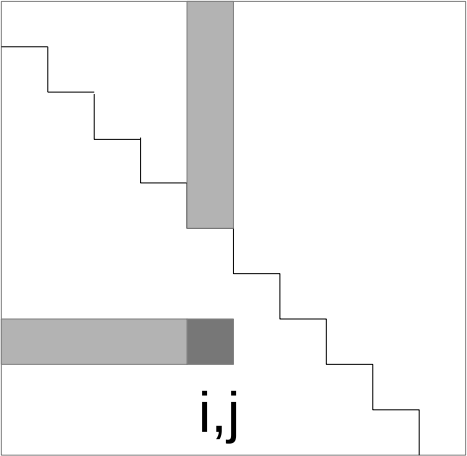
\includegraphics[width=.8\textwidth, keepaspectratio]{images/ch2/LU_decomposition_crout_method_visualization_elements_used_simple_lower.png}
		\label{Figure:implementation-decomposition-project-lu-decomposition-element-dependance-lower}
	\end{subfigure}%
	\begin{subfigure}{.5\textwidth}
		\centering
		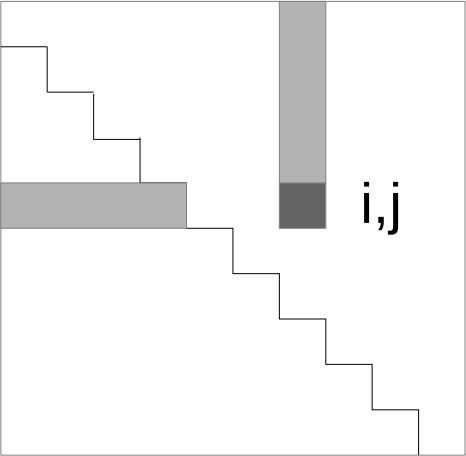
\includegraphics[width=.8\textwidth, keepaspectratio]{images/ch2/LU_decomposition_crout_method_visualization_elements_used_simple_upper.png}
		\label{Figure:implementation-decomposition-project-lu-decomposition-element-dependance-upper}
	\end{subfigure}
	\caption{Examples showing the elements used (shaded regions) to calculate an element at row $ i $ and column $ j $ (dark square). As described earlier, only elements with indices in the interval $ \left[0, \min(i, j)\right] $ are used in the element's row and column. Taken from E. Chow's and A. Patel's \emph{Fine-Grained Parallel Incomplete LU Factorization} \cite{Chow2015}.}
	\label{Figure:implementation-decomposition-project-lu-decomposition-element-dependance}
\end{figure}

The implementation of the Iterative Crout method for the GPU using matrix $ \mathbb{Z} $ is shown in Listing~\ref{Listing:implementation-decomposition-project-lu-decomposition-iterative-crout-method-convergence-by-sections}. The listing does not contain the decomposition kernel itself as it is shown later in Listing~\ref{Listing:implementation-decomposition-project-lu-decomposition-iterative-crout-method-convergence-of-single-section} in \textit{\nameref{Subparagraph:implementation-decomposition-project-lu-decomposition-iterative-crout-method-convergence-of-single-section}}.

\begin{lstlisting}[caption={GPU implementation of the Iterative Crout method. Some code has been omitted as it is not important for the description, for example, checking if the input matrix is square. Overall, the code performs the following: initialization of variables (including CUDA grid specifications, page-locked host memory, streams, etc.), then the entire matrix $ \mathbb{A} $ is decomposed using the \textit{Convergence by sections} concept. The constant \code{BLOCK\_SIZE} dictates how many threads are present in a single thread block. The \code{converged\_host} variable is purposefully initialized using page-locked host memory as its value is copied between the host and device in every iteration of the do-while loop. Thus, as described in \textit{\nameref{Paragraph:CUDA-memory-management-page-locked-host-memory}} in Section~\ref{Paragraph:CUDA-memory-management-page-locked-host-memory}, the higher bandwidth provided can help reduce the overall time spent copying during computation. Taken from the Decomposition project repository on GitLab\protect\footref{Footnote:decomposition-project-gitlab-url}.},label={Listing:implementation-decomposition-project-lu-decomposition-iterative-crout-method-convergence-by-sections},escapechar=@]
template< typename Matrix1,	typename Matrix2 >
void CroutMethodIterative::decompose( Matrix1& A, Matrix2& Z )
{
	using Real   = typename Matrix1::RealType;
	using Device = typename Matrix1::DeviceType;
	using Index  = typename Matrix1::IndexType;
	
	Index num_rows = A.getRows();
	Index num_cols = A.getColumns();
	
	Matrix2 Znew;
	Znew.setLike( Z );
	Z = A;
	bool converged = true;
	Real tolerance = 0;
	
	// Compute the size of a section
	Index sectionSize = min( max( num_cols / 10, (Index)256 ), (Index)1024 );
	sectionSize = ( sectionSize + BLOCK_SIZE - 1 ) / BLOCK_SIZE * BLOCK_SIZE;
	
	// Determine the number of blocks based on the section size
	Index blocks = sectionSize / BLOCK_SIZE;
	dim3 threadsPerBlock( BLOCK_SIZE, BLOCK_SIZE );
	dim3 blocksPerGrid( blocks, blocks );
	
	// Copy required data to the GPU
	Matrix1* matrixA_kernel     = TNL::Cuda::passToDevice( A );
	Matrix2* matrixZ_kernel     = TNL::Cuda::passToDevice( Z );
	Matrix2* matrixZnew_kernel  = TNL::Cuda::passToDevice( Znew );
	bool*    converged_kernel   = TNL::Cuda::passToDevice( converged );
	Real*    tolerance_kernel   = TNL::Cuda::passToDevice( tolerance );
	
	// Initialize the converged switch to page-locked host memory
	bool* converged_host = NULL;
	cudaMallocHost( (void **) &converged_host, sizeof(bool) );
	
	// Allocate and initialize an array of 2 stream handles
	int nstreams = 2;
	cudaStream_t *streams = (cudaStream_t *)malloc( nstreams * sizeof(cudaStream_t) );
	for( int i = 0; i < nstreams; ++i ) {
		cudaStreamCreate( &(streams[i] ) );
	}
	
	// Initialize variables for keeping track of where the main diagonal section begins and ends
	Index diag_start, diag_end, sStart, sEnd;
	
	// Converge by sections
	for( diag_start = 0, diag_end = min( num_cols, sectionSize ); diag_start < diag_end; diag_start += sectionSize, diag_end = min( num_cols, diag_end + sectionSize ) ) {
		// Converge the diagonal section first using the Default stream
		do {
			*converged_host = true;
			cudaMemcpy( converged_kernel, converged_host, sizeof(bool), cudaMemcpyHostToDevice );
			
			DecomposeKernel< Real, Index ><<< blocksPerGrid, threadsPerBlock >>>( matrixA_kernel, matrixZ_kernel, matrixZnew_kernel, diag_start, diag_end, diag_start, diag_end, tolerance_kernel, converged_kernel );
			
			// Synchronize after execution of kernel before copying value of converged
			cudaDeviceSynchronize();@\label{Line:decompose-method-cudaDeviceSynchronize-1}@
			cudaMemcpy( converged_host, converged_kernel, sizeof(bool), cudaMemcpyDeviceToHost );
		} while( !*converged_host );
		
		// Converge sections below and to the right of the main diagonal section using the two streams
		for( sStart = diag_end, sEnd = min( num_cols, diag_end + sectionSize );	sStart < sEnd;	sStart += sectionSize, sEnd = min( num_cols, sEnd + sectionSize ) ) {
			do {
				*converged_host = true;
				cudaMemcpy( converged_kernel, converged_host, sizeof(bool), cudaMemcpyHostToDevice );
				
				// Run Stream 1: iterate columns - rows should stay the same
				DecomposeKernel< Real, Index ><<< blocksPerGrid, threadsPerBlock, 0, streams[0] >>>( matrixA_kernel, matrixZ_kernel, matrixZnew_kernel, sStart, sEnd, diag_start, diag_end, tolerance_kernel, converged_kernel );
				
				// Run Stream 2: iterate rows - columns should stay the same
				DecomposeKernel< Real, Index ><<< blocksPerGrid, threadsPerBlock, 0, streams[1] >>>( matrixA_kernel, matrixZ_kernel, matrixZnew_kernel, diag_start, diag_end, sStart, sEnd, tolerance_kernel, converged_kernel );
				
				// Synchronize after execution of kernels before copying value of converged
				cudaDeviceSynchronize();@\label{Line:decompose-method-cudaDeviceSynchronize-2}@
				cudaMemcpy( converged_host, converged_kernel, sizeof(bool), cudaMemcpyDeviceToHost );
			} while( !*converged_host );
		}
	}
}
\end{lstlisting}

One of the first performance-determining aspects shown in Listing~\ref{Listing:implementation-decomposition-project-lu-decomposition-iterative-crout-method-convergence-by-sections} is the size of a section (\code{sectionSize} or $ s $). It affects both the speed of computation and the accuracy of results (detailed further in Chapter~\ref{Chapter:benchmark-results}). Specifically, the phrase "\textit{accuracy of results}" refers to how much the matrix resulting from $ \mathbb{L}\cdot\mathbb{U} $ differs from the original input matrix $ \mathbb{A} $. How the size of a section is calculated changed many times throughout development. Initially, the size of a section is set to $ 1/10 $ of the dimensions of $ \mathbb{Z} $, however, this value must be within the interval $ \left[256, 1024\right] $. If it is outside of this interval, then the size is set to the interval's closest endpoint (256 or 1024). Then, its value is rounded to the nearest multiple of \code{BLOCK\_SIZE} (8, 16, or 32) that is larger than the original \code{sectionSize} due to CUDA-related reasons described later in \textit{\nameref{Subparagraph:implementation-decomposition-project-lu-decomposition-iterative-crout-method-convergence-of-single-section}}. \\
As can be seen in Listing~\ref{Listing:implementation-decomposition-project-lu-decomposition-iterative-crout-method-convergence-by-sections} each section is converged using a decomposition kernel. Since each kernel is launched on a grid of blocks that are made up of threads, then each section is converged using a grid. Thus, in order to facilitate parallel convergence of sections, CUDA streams (detailed in Section~\ref{Subsubsection:CUDA-asynchronous-concurrent-execution-concurrent-streams}) were used. Specifically, sections that encompass the main diagonal (main diagonal sections) are converged using the default stream and sections converged in parallel were each given a separate stream, i.e. two streams are created and each is used to converge one of the parallel sections. For example - using the numbering of sections from Figure~\ref{Figure:implementation-decomposition-project-lu-decomposition-order-of-convergence-of-sections} - first, section '$ 0 $' is converged using the default stream. Then, sections labeled with a '$ 1 $' are converged - each using a different stream. Following that, sections labeled with a '$ 2 $' are converged - each using a different stream - and so on until sections labeled with a '$ 3 $'. Then section '$ 4 $' is converged, again using the default stream. \\
In Figure~\ref{Figure:implementation-decomposition-project-lu-decomposition-order-of-convergence-of-sections} it can be seen that some sections are converged in parallel. In general, a section can be converged optimally only if specific sections above and to the left of it are already converged. The specific sections that the to-be-converged section depends are the same as the elements required to converge a specific element quickly. In order to imagine this better, the dark square in Figure~\ref{Figure:implementation-decomposition-project-lu-decomposition-element-dependance} can be considered as the to-be-converged section and the shaded regions can be considered as the sections that must be converged before it. It is noteworthy that the general concept - how a section can be converged optimally - allows for more than two sections to be converging simultaneously. This and any other potential performance improvements are detailed in Section~\ref{Section:implementation-optimization}. \\
In summary, converging the input matrix by sections is faster than converging all of it at once since its elements - especially those in the lower-right corner - will have higher quality elements available for the computation of their value. For example, let $ z_{ij} $ (located in the lower-right corner of $ \mathbb{Z} $) be the currently computed element. If the entire matrix $ \mathbb{Z} $ is being converged at once and if it is a large matrix, then, since elements in the first few rows and columns (excluding the 1st row and column as their values are taken directly from $ \mathbb{A} $ and not altered further) are highly inaccurate they will cooperatively produce even less accurate elements in the later rows and columns - a snowball effect of low quality elements. Thus, during the first few iterations $ z_{ij} $ will be calculated using low quality elements and it will be far from its final converged value. Slowly, through multiple iterations the quality of elements will increase row-by-row and column-by-column which will in turn slowly converge $ z_{ij} $. Thus, when converging the entire matrix simultaneously, computing elements found further in the matrix (elements near and in the lower-right corner of the matrix) is a waste of resources and time. Ultimately, this makes convergence by sections more optimal.

\subparagraph{Convergence of a single section}\label{Subparagraph:implementation-decomposition-project-lu-decomposition-iterative-crout-method-convergence-of-single-section}
While the previous part detailed how an entire matrix is converged by sections, this part describes how a single section is converged. A single section denotes a $ s\times s $ sub-matrix of matrix $ \mathbb{Z} $ that is labeled $ \mathbb{Z}_{sub} $. Since the sub-matrix (section) is not being decomposed itself as a matrix, rather this part of matrix $ \mathbb{Z} $ is being decomposed, then, the phrase "\textit{single section is converged}" is befitting. In technical terms this means providing a series of inputs (sub-matrices, indexes, tolerance values, etc.) to a kernel that is executed on the device. First, for the explanation of the decomposition kernel, it is necessary to slightly alter the algorithm from Section~\ref{Subsection:LU-decomposition-numerical-method} - using matrix $ \mathbb{Z} $ instead of $ \mathbb{L} $ and $ \mathbb{U} $ - to the perspective of a section:

\begin{enumerate}
	\item Given input matrices $ \mathbb{A} $ and $ \mathbb{Z}^t $ calculate the next iteration of a specific sub-matrix: $ \mathbb{Z}^{t+1}_{sub} $:
		\begin{align}
			z_{ij}^{t+1} &= a_{ij} - \sum_{k=1}^{j-1}z_{ik}^{t}z_{kj}^{t}                                                              &\quad i \geq j \nonumber\,, \\
			z_{ij}^{t+1} &= \frac{1}{z_{ii}^{t}} \left ( z_{ij} - \sum_{k=1}^{i-1}z_{ik}^{t}z_{kj}^{t} \right ) &\quad i < j \nonumber\,.\\
		\end{align}
	\item Check if the section has converged according to the tolerance rule: $ \left | \mathbb{Z}^{t+1}_{sub} - \mathbb{Z}^{t}_{sub} \right | > tol $ (where $ tol $ is some hard-set value, for example, $ 0.0001 $). If the tolerance rule has not passed, then go back to step 2.
	\item If the tolerance rule has passed, then the algorithm has arrived to an approximate solution of a sub-matrix in $ \mathbb{L}\mathbb{U} $ (stored in $ \mathbb{Z} $).
\end{enumerate}

Note that the value of the $ tol $ parameter is another important factor that determines the performance (speed of execution and accuracy of results). If the value of the parameter is too high, for example, $ 1.5 $ then the algorithm will converge faster, however, the matrix resulting from $ \mathbb{L}\mathbb{U} $ will differ more significantly from $ \mathbb{A} $, i.e. the decomposition will be inaccurate. On the other hand, the closer the tolerance value is to zero, the more accurate the results will be, however, it will take longer for the algorithm to converge. This parameter went through many changes, before finally settling to $ 0.0 $. The reasons behind this decision were the following:

\begin{itemize}
	\item \textit{\nameref{Subparagraph:implementation-decomposition-project-lu-decomposition-iterative-crout-method-convergence-by-sections}} allows for greater granularity as the quality of each $ s \times s $ section depends on the quality of specific sections that were converged before it. Thus, setting the tolerance parameter to zero means that the elements of a section are computed using elements that are as accurate as possible.
	\item Testing the solution on a set of matrices that comprised of 61 sparse, dense, small and large matrices revealed that the difference in performance when setting the tolerance value near zero (for example, $ 0.0001 $) and just zero was negligible. However, the accuracy of results when $ tol = 0.0 $ was significantly higher - detailed further in Section~\ref{Section:implementation-optimization} and Chapter~\ref{Chapter:benchmark-results}.
	\item The testing further revealed that the accuracy of results can decrease if the dimensions of the input matrix increase. Thus, it was decided that even though speed of convergence is important, it loses meaning if the produced results are unusable.
\end{itemize}

The implementation of the decomposition kernel using matrix $ \mathbb{Z} $ is shown in Listing~\ref{Listing:implementation-decomposition-project-lu-decomposition-iterative-crout-method-convergence-of-single-section}.

\begin{lstlisting}[caption={The constant \code{BLOCK\_SIZE} is by default hard-coded to be equal to 8 in the \code{CroutMethodIterative} header file using the \code{\#define} macro. The kernel takes matrices $ \mathbb{A} $, $ \mathbb{Z} $ (iteration $ t $ of $ \mathbb{Z} $), and $ \mathbb{Z}_{new} $ (iteration $ t+1 $ of $ \mathbb{Z} $) as input parameters, and uses other input variables to offset the threads in the grid so that only a specific section of $ \mathbb{Z} $ is computed. Note that the kernel is not part of the \code{CroutMethodIteartive} class since kernels cannot be members of a class - as mentioned in \textit{\nameref{Paragraph:CUDA-C++-extensions-outer-kernel-extensions-function-extensions}} in Section~\ref{Paragraph:CUDA-C++-extensions-outer-kernel-extensions-function-extensions} - however, it is located in the same file that it is called from. Taken from the Decomposition project repository on GitLab\protect\footref{Footnote:decomposition-project-gitlab-url}.},label={Listing:implementation-decomposition-project-lu-decomposition-iterative-crout-method-convergence-of-single-section},escapechar=@]
template< typename Real, typename Index, typename Matrix1, typename Matrix2 >
__global__ void DecomposeKernel( const Matrix1* _A, Matrix2* _Z, Matrix2* _Znew, const Index col_sStart, const Index col_sEnd, const Index row_sStart, const Index row_sEnd, const Real* tolerance, bool* converged )
{
	auto& A = *_A; auto& Z = *_Z; auto& Znew = *_Znew;
	
	// Get a thread's sub-matrix ID that is offset to become a global ID of Z
	Index row = blockIdx.y * blockDim.y + threadIdx.y + row_sStart;
	Index col = blockIdx.x * blockDim.x + threadIdx.x + col_sStart;
	
	Index tx = threadIdx.x;
	Index ty = threadIdx.y;
	Real sum = 0;
	
	// Set overreaching thread ID to the closest edge of the matrix's dimensions
	Index max_col = col_sEnd - 1;
	Index max_row = row_sEnd - 1;
	Index new_row = min( row, max_row );
	Index new_col = min( col, max_col );
	
	// Get the smallest index of the thread's element and offset it by BLOCK_SIZE - preparation for the use of shared memory
	Index min_row_col = min( new_row, new_col ) - BLOCK_SIZE;
	
	// Initialize shared memory
	__shared__ Real ZsLower[BLOCK_SIZE][BLOCK_SIZE];
	__shared__ Real ZsUpper[BLOCK_SIZE][BLOCK_SIZE];
	
	Index i, k;
	
	// Compute the sum needed for element (row, col) by loading blocks of elements from global to shared memory and multiplying them
	for( i = 0; i <= min_row_col; i += BLOCK_SIZE ) {
		ZsLower[ty][tx] = Z( new_row, i + tx );
		ZsUpper[ty][tx] = Z( i + ty, new_col );
		
		__syncthreads();
		
		#pragma unroll
		for( k = 0; k < BLOCK_SIZE; ++k ) {
			sum += ZsLower[ty][k] * ZsUpper[k][tx]; @\label{Line:decomposition-kernel-shared-memory-correct-usage-1}@
		}
		__syncthreads();
	}
	
	// Loop unrolling means looping by multiples of BLOCK_SIZE @\label{Line:decomposition-kernel-loop-unrolling-begin}@
	// If the number of remaining elements is less than BLOCK_SIZE, then compute them separately
	ZsLower[ty][tx] = Z( new_row, min( i + tx, max_col ) );
	ZsUpper[ty][tx] = Z( min( i + ty, max_row ), new_col );
	__syncthreads();
	Index t_to_use = row >= col ? tx : ty;
	for( k = 0; k < t_to_use; ++k ) {
		sum += ZsLower[ty][k] * ZsUpper[k][tx]; @\label{Line:decomposition-kernel-shared-memory-correct-usage-2}@
	} @\label{Line:decomposition-kernel-loop-unrolling-end}@
	
	//  Terminate threads whose ID reaches out of matrix dimensions @\label{Line:decomposition-kernel-terminate-threads-begin}@
	if( row >= row_sEnd || col >= col_sEnd ) {
		return;
	} @\label{Line:decomposition-kernel-terminate-threads-end}@
	
	// Compute the value of element (row, col) in the new iteration
	if( row >= col ) {
		Znew( row, col ) = A( row, col ) - sum;
	} else {
		if( Z( row, row ) == 0 ) {
			printf( "Key element: %f\t(row:%d, col:%d)\n", Z( row, row ), (int)row, (int)col );
			assert( Z( row, row ) != 0 );
		}

		Znew( row, col ) = ( A( row, col ) - sum ) / Z( row, row );
	}
	
	// Check if the element (row, col) has converged
	if( abs( Znew( row, col ) - Z( row, col ) ) > *tolerance ) {
		*converged = false;
	}
	
	// Assign element for this iteration
	Z( row, col ) = Znew( row, col );
}
\end{lstlisting}

The kernel presented in Listing~\ref{Listing:implementation-decomposition-project-lu-decomposition-iterative-crout-method-convergence-of-single-section} has the following input parameters:

\begin{itemize}
	\item \code{col\_sStart} - Starting column index of the section in matrix $ \mathbb{Z} $.
	\item \code{col\_sEnd} - Ending column index of the section in matrix $ \mathbb{Z} $.
	\item \code{row\_sStart} - Starting row index of the section in matrix $ \mathbb{Z} $.
	\item \code{row\_sEnd} - Ending row index of the section in matrix $ \mathbb{Z} $.
	\item \code{tolerance} - Tolerance parameter stored in global memory of the device. All threads only need to read it in order to check the tolerance rule for their element.
	\item \code{converged} - Boolean switch stored in global memory of the device that determined whether element \code{(row, col)} has converged. At the end of the kernel, each thread evaluates whether its element has converged according to the convergence rule describe above. While it is generally considered bad practice for multiple threads to write to a single address in memory, in this instance, is it befitting. The reasoning is that for the algorithm to perform another iteration, only one thread needs to set \code{converged = false}. As long the value of \code{converged} is copied from the device to the host after all threads have finished executing the kernel, then the intended behavior occurs. This is assured using the \code{cudaDeviceSynchronize()} function used in lines~\ref{Line:decompose-method-cudaDeviceSynchronize-1} and \ref{Line:decompose-method-cudaDeviceSynchronize-2} in Listing~\ref{Listing:implementation-decomposition-project-lu-decomposition-iterative-crout-method-convergence-by-sections} as explained in \textit{\nameref{Paragraph:CUDA-asynchronous-concurrent-execution-streams-explicit-synchronization}} in Section~\ref{Paragraph:CUDA-asynchronous-concurrent-execution-streams-explicit-synchronization}.
\end{itemize}

From the parameters listed above, the first four are used to determine where in matrix $ \mathbb{Z} $ the thread's element is located. Together, the threads then converge the elements of the intended section. The remaining input parameters are specifically prefixed with a \code{\_} as they are not used, instead, pointers to their memory address are initialized in such a way that allows for clean use of the overloaded \code{operator()} which is detailed \textit{\nameref{Paragraph:implementation-tnl-library-dense-matrix}} in Section~\ref{Paragraph:implementation-tnl-library-dense-matrix}. \\
Furthermore, other than the input parameters and CUDA-related extensions detailed \textit{\nameref{Subsubsection:CUDA-C++-extensions-inter-kernel-extensions}} in Section~\ref{Subsubsection:CUDA-C++-extensions-inter-kernel-extensions} the kernel also has access to the macro-defined \code{BLOCK\_SIZE} variable. The \code{BLOCK\_SIZE} constant is set using the \code{\#define} macro to make the compiler unroll the \code{for} loop during compile time using \code{\#pragma unroll}. Loop unrolling is a compiler optimization that reduces the work done by the processing thread. Specifically, it removes the need for the processing thread to initialize the loop variable, evaluate the condition and increment the variable \cite{Cardoso2017}. However, if the number of loops in a \code{for} loop is now known during compile time, then the loop cannot be unrolled. An example showing loop unrolling is shown in Listing~\ref{Listing:implementation-decomposition-project-lu-decomposition-iterative-crout-method-loop-unrolling}.

\begin{lstlisting}[caption={Example demonstrating loop unrolling. In this specific case, if loop unrolling is used, then the processor will not have to: initialize \code{k}, evalute \code{k < BLOCK\_SIZE} nine times and increment \code{k} eight times. If \code{BLOCK\_SIZE} would be obtained as an input parameter, then the loop would not be unrolled as the input parameter is not known during compile time. Taken from \emph{Embedded Computing for High Performance} \cite{Cardoso2017}.},label={Listing:implementation-decomposition-project-lu-decomposition-iterative-crout-method-loop-unrolling}]
// Hard-set constant - value is known by the compiler at compile time
#define BLOCK_SIZE 8

// Original for loop
for( k = 0; k < BLOCK_SIZE; ++k ) {
	sum += ZsLower[ty][k] * ZsUpper[k][tx];
}

// For loop transformed using loop unrolling during compilation
sum += ZsLower[ty][0] * ZsUpper[0][tx];
sum += ZsLower[ty][1] * ZsUpper[1][tx];
sum += ZsLower[ty][2] * ZsUpper[2][tx];
sum += ZsLower[ty][3] * ZsUpper[3][tx];
sum += ZsLower[ty][4] * ZsUpper[4][tx];
sum += ZsLower[ty][5] * ZsUpper[5][tx];
sum += ZsLower[ty][6] * ZsUpper[6][tx];
sum += ZsLower[ty][7] * ZsUpper[7][tx];
\end{lstlisting}

Another important aspect of the implementation lies at the core of the kernel: use of shared memory. Since each section is assigned a grid made up of blocks, then each block has limited shared memory available to it as described in \textit{\nameref{Paragraph:CUDA-memory-management-shared-memory}} in Section~\ref{Paragraph:CUDA-memory-management-shared-memory}. Overall, shared memory is used exactly as described in the matrix multiplication \textit{\nameref{Subsubsection:CUDA-matrix-multiplication-example-with-shared-memory}} in Section~\ref{Subsubsection:CUDA-matrix-multiplication-example-with-shared-memory} with an exception. In the example - depicted in Figure~\ref{Figure:CUDA-matrix-multiplication-with-shared-memory-example} - the blocks loop through the entire matrix. As explained earlier in \textit{\nameref{Subparagraph:implementation-decomposition-project-lu-decomposition-iterative-crout-method-convergence-by-sections}} in Section~\ref{Subparagraph:implementation-decomposition-project-lu-decomposition-iterative-crout-method-convergence-by-sections} and shown in Figure~\ref{Figure:implementation-decomposition-project-lu-decomposition-element-dependance} using all elements in the row and column of an element is not required. Thus, in this implementation, the thread block finishes looping once the last required block of elements is used for the computation. However, this presented an obstacle if loop unrolling is used as it was on line~\ref{Line:matrix-multiplication-pragma-unroll} in the example code attached in Listing~\ref{Listing:CUDA-matrix-multiplication-full-code} of Attachment~\ref{Attachment:CUDA-matrix-multiplication-code}. The obstacle is that once the thread block arrives to the last block of elements required for the computation, it must stop at specific elements, i.e. each thread needed to stop at a different element. In other words, the number of loops required for each thread in the last block of elements is not known at compile time. This means that loop unrolling is not possible for the last block of required elements and it can only be performed for the blocks before. For this purpose the variable \code{min\_row\_col} is offset by \code{BLOCK\_SIZE} to make the loop using loop unrolling end sooner. The remaining elements are then computed using a regular \code{for} loop (lines \ref{Line:decomposition-kernel-loop-unrolling-begin} - \ref{Line:decomposition-kernel-loop-unrolling-end} in Listing~\ref{Listing:implementation-decomposition-project-lu-decomposition-iterative-crout-method-convergence-of-single-section}). \\
As detailed in \textit{\nameref{Paragraph:CUDA-memory-management-shared-memory}} in Section~\ref{Paragraph:CUDA-memory-management-shared-memory} when using shared memory, it is important to avoid a bank conflict. In the kernel shown in Listing~\ref{Listing:implementation-decomposition-project-lu-decomposition-iterative-crout-method-convergence-of-single-section} shared memory is read from only on lines~\ref{Line:decomposition-kernel-shared-memory-correct-usage-1} and \ref{Line:decomposition-kernel-shared-memory-correct-usage-2}. Specifically, in the multiplication operation \code{ZsLower[ty][k] * ZsUpper[k][tx]} shared memory is being read from in two different ways (also detailed in \textit{\nameref{Paragraph:CUDA-memory-management-shared-memory}} in Section~\ref{Paragraph:CUDA-memory-management-shared-memory}):

\begin{itemize}
	\item \code{ZsLower[ty][k]} - All threads in a warp have the same \code{ty} id. This means that for a given \code{k} all threads of a warp access the same location in shared memory - known as a \textit{Broadcast} - which is a fast data-serving strategy.
	\item \code{ZsUpper[k][tx]} - Each thread in a warp has a unique and linearly increasing \code{tx}. This means that for a given \code{k} each thread of a warp accesses one word in a different bank. In other words, a single word is requested from each bank by a unique thread, thus, all 32 threads of a warp are served by all 32 banks simultaneously and expeditiously.
\end{itemize}

In \textit{\nameref{Subparagraph:implementation-decomposition-project-lu-decomposition-iterative-crout-method-convergence-by-sections}}, it was mentioned that the size of a section must be a multiple of \code{BLOCK\_SIZE}. Although \code{sectionSize} is not used directly in the kernel, the use of shared memory needed to be explained in order to present the reasoning for this limitation. Lines ~\ref{Line:decomposition-kernel-terminate-threads-begin} - \ref{Line:decomposition-kernel-terminate-threads-end} in Listing~\ref{Listing:implementation-decomposition-project-lu-decomposition-iterative-crout-method-convergence-of-single-section} show that any threads whose shifted global ID overreaches the matrix dimensions are terminated. In a typical CUDA kernel, this step would be performed near the beginning of the kernel. However, in this case, the threads that overreach are needed for loading data from global to shared memory. For example, looking at Figure~\ref{Figure:CUDA-matrix-multiplication-with-shared-memory-example}, if the matrix dimensions were not a multiple of \code{BLOCK\_SIZE} and the blocks computing the last columns were partly outside of matrix dimensions, then the of right-most threads of the upper block (matrix $ \mathbb{B} $) would reach out of matrix dimensions and they should - under normal circumstances - be terminated to avoid erroneous behavior. However, the same threads are concurrently being used to load data from global to shared memory in the left block (matrix $ \mathbb{A} $) - there the threads would not reach out of bounds. For this reason, the threads cannot be terminated when computing the sum and that is also the reason why their cut global ID is used during calculation. The threads mentioned compute sums identical to the threads whose global ID is on the edge of the matrix's dimensions. Then, the values computed by the cut threads is discarded once they are terminated. Thus, if \code{sectionSize} is not a multiple of \code{BLOCK\_SIZE}, then loop unrolling would not be possible as the block of elements loaded into shared memory would not cover the entire section.


\subsection{Benchmark \TO}\label{Subsection:implementation-decomposition-project-benchmark}
As mentioned in \textit{\nameref{Paragraph:implementation-decomposition-project-lu-decomposition-implementation-requirements}} in Section~\ref{Paragraph:implementation-decomposition-project-lu-decomposition-implementation-requirements} one of the goals of this project was to measure the acceleration of the GPU version of the LU decomposition against the CPU version. For this purpose a benchmark system was implemented. In its majority, the structuring and code was adopted from the SpMV TNL Benchmark structure\footnote{TNL SpMV Benchmark GitLab repository URL: \url{https://gitlab.com/tnl-project/tnl/-/tree/main/src/Benchmarks/SpMV}} which was implemented by one of the main developers for TNL, Ph.D. student Jakub Klinkovský. However, some logic was reworked specifically for this project. \\
The benchmarking procedure is initiated from a Bash script\footnote{Benchmark script URL in the Decomposition GitLab repository: \url{https://mmg-gitlab.fjfi.cvut.cz/gitlab/tnl/lu-decomposition/-/blob/master/src/Benchmark/scripts/run-decomposition-benchmark}} and it involves running the entire benchmark six times. Specifically, for each precision (single or double) it is run three times - each with a different number of threads per block: $ 8 $, $ 16 $, or $ 32 $; i.e. blocks of $ 8 \times 8 $, $ 16 \times 16 $, or $ 32 \times 32 $ threads. More threads per block are not possible since the maximum numbers of threads per block is 1024 - detailed in \textit{\nameref{Paragraph:CUDA-thread-management-block}} in Section~\ref{Paragraph:CUDA-thread-management-block}. While the "\textit{threads-per-block}" part of the benchmark was initially added to determine the optimal number of threads per block, it was never apparent from any benchmark run which value is optimal, therefore, it was kept for future development. Each run of the benchmark involves decomposing a set of matrices; each matrix is stored in an \code{.mtx} file. Specifically, the subroutine for benchmarking a matrix is as follows (assuming the \code{precision} and \code{threads-squared-per-block} arguments are set):

\begin{enumerate}
	\item Load the matrix from its \code{.mtx} file using the \code{MatrixReader} class implemented in TNL\footnote{\code{MatrixReader} class header file in the TNL GitLab repository URL: \url{https://gitlab.com/tnl-project/tnl/-/blob/main/src/TNL/Matrices/MatrixReader.h}} to an instance of \code{DenseMatrix}.
	\item Compute the decomposition using the CPU implementation of the Crout method described in \textit{\nameref{Paragraph:implementation-decomposition-project-lu-decomposition-crout-method}} in Section~\ref{Paragraph:implementation-decomposition-project-lu-decomposition-crout-method} and, if specified, compute the maximum difference of $ \left| \mathbb{A} - \mathbb{L}\mathbb{U} \right| $. Then, log statistics such as execution time, bandwidth achieved, maximum difference, etc. into the log file.
	\item Compute the decomposition using the GPU implementation of the Iterative Crout method described in \textit{\nameref{Paragraph:implementation-decomposition-project-lu-decomposition-iterative-crout-method}} in Section~\ref{Paragraph:implementation-decomposition-project-lu-decomposition-iterative-crout-method} and, if specified, compute the maximum difference of $ \left| \mathbb{A} - \mathbb{L}\mathbb{U} \right| $. Then, log statistics such as execution time, bandwidth achieved, maximum difference, etc. into the log file.
\end{enumerate}

Additionally, the log file can be transformed into an HTML table and data such as bandwidth and relative speedup can be plotted into graphs using a convenient Python script\footnote{Transforming Python script GitLab repository URL: \url{https://mmg-gitlab.fjfi.cvut.cz/gitlab/tnl/lu-decomposition/-/blob/master/src/Benchmark/scripts/decomposition-benchmark-make-tables-json.py}} - originally adopted from TNL and later modified. \\
As mentioned in Section~3.2 of the author's bachelor thesis \textit{Formats for storage of sparse matrices on GPU} \cite{Cejka2020}, benchmarks can be used to identify issues missed by unit tests. This claim persisted during the development of this project as some matrices were too large to be stored using \code{DenseMatrix} on the GPU. Furthermore, the benchmark implementation played a crucial role when optimizing the solution.



\section{Optimization \TO}\label{Section:implementation-optimization}
In the preceding sections, it was mentioned that the \textit{Decomposition} project went through various optimizations during development. This section aims to summarize the evolution of the GPU LU decomposition implementation from its initial naive version to its present form. Additionally, a selection of concepts that were attempted, but ultimately ended up being sub-optimal will also be described. The performance of each change was measured by running the benchmark on a set of 50 sparse and dense matrices with varying dimensions between $ 27 \times 27 $ and $ 10581 \times 10581 $. This section will not present specific results (execution time, bandwidth, etc.), nor will some of the matrices will be presented or described in greater detail; that will be shown in Chapter~\ref{Chapter:benchmark-results}.

\paragraph{Initial naive implementation}\label{Paragraph:implementation-optimization-initial-naive-implementation}
The initial naive implementation was designed in such a manner where the entire matrix was decomposed by a single CUDA grid. In other words, each thread would compute one element in each iteration, then, the tolerance rule would be imposed (with $ tol = 0.001 $). The kernel and how convergence was handled withing \code{CroutMethodIterative::decompose()} is shown in Listing~\ref{Listing:implementation-optimization-initial-naive-implementation}.

\begin{lstlisting}[caption={Initial naive implementation of the GPU version of the Iterative Crout method. Taken from the Decomposition project repository on GitLab\protect\footref{Footnote:decomposition-project-gitlab-url}.},label={Listing:implementation-optimization-initial-naive-implementation},escapechar=@]
template< typename Real, typename Index, typename Matrix1, typename Matrix2 >
__global__ void DecomposeKernel( const Matrix1* A, Matrix2* Z, Matrix2* Znew, Index row_size )
{
	int row = blockIdx.y * blockDim.y + threadIdx.y;
	int col = blockIdx.x * blockDim.x + threadIdx.x;
	
	if( row < row_size && col < row_size ) { @\label{Line:initial-naive-implementation-thread-divergence-1}@
		Index k;
		Real sum = 0;
		
		if( row >= col ) {  @\label{Line:initial-naive-implementation-thread-divergence-2}@
			sum = 0;
			for( k = 0; k < col; k++ ) {
				sum = sum + Z->getElement( row, k ) * Z->getElement( k, col );
			}
			
			Znew->setElement( row, col, A->getElement( row, col ) - sum );
		}
		else {
			TNL_ASSERT( Z->getElement( row, row ) != 0,	std::cerr << "Z( " << row << ", " << row << " ) = 0. Cannot divide by 0!" << std::endl );
			sum = 0;
			for( k = 0; k < row; k++ ) {
				sum = sum + Z->getElement( row, k ) * Z->getElement( k, col );
			}
			
			Znew->setElement( row, col, ( A->getElement( row, col ) - sum ) / Z->getElement( row, row ) );
		}
	} @\label{Line:initial-naive-implementation-thread-divergence-end}@
}

template< typename Matrix1, typename Matrix2 > @\label{Line:initial-naive-implementation-convergence-checking-begin}@
void CroutMethodIterative::decompose( Matrix1& A, Matrix2& Z )
{
	// ...
	do {
		DecomposeKernel< RealType, IndexType, Matrix1, Matrix2 ><<< blocksPerGrid, threadsPerBlock >>>( matrix1_kernel, matrix2_kernel, matrix2new_kernel, num_rows );
		
		// Determine if Z has converged by computing the maximum absolute difference between Z and Znew, and comparing it with a hard-set tolerance
		converged = matrixDifferenceTolerable( Znew, Z ); @\label{Line:initial-naive-implementation-convergence-checking}@
		
		Z = Znew;
	} while( !converged );
	// ...
} @\label{Line:initial-naive-implementation-convergence-checking-end}@
\end{lstlisting}

As can be seen in Listing~\ref{Listing:implementation-optimization-initial-naive-implementation}, the implementation had several drawbacks:

\begin{itemize}
	\item The condition on line~\ref{Line:initial-naive-implementation-thread-divergence-1} caused divergence of threads (described in \textit{\nameref{Paragraph:CUDA-thread-management-warp}} in Section~\ref{Paragraph:CUDA-thread-management-warp}). However, this affected only the warps whose threads would overreach the matrix dimensions.
	\item The condition on line~\ref{Line:initial-naive-implementation-thread-divergence-2} also caused divergence of threads. However, in this instance the majority of warps were affected.
	\item All operations with elements of the input matrices are done in the device's global memory. Reading from global memory is sub-optimal compared to reading from shared memory, however, global memory bandwidth is even lower if the access to memory is not coalesced. Since the number of loops each thread performed in its \code{for} differed, then further thread divergence and non-coalesced memory access occurred as a consequence.
	\item The inefficient convergence described at the end of \textit{\nameref{Subparagraph:implementation-decomposition-project-lu-decomposition-iterative-crout-method-convergence-by-sections}} in Section~\ref{Subparagraph:implementation-decomposition-project-lu-decomposition-iterative-crout-method-convergence-by-sections} is precisely the means of convergence used in this naive implementation.
\end{itemize}

In summary, this implementation was sub-optimal, however, it served as a foundation for future development.

\paragraph{Dynamic parallelism}\label{Paragraph:implementation-optimization-dynamic-parallelism}
Following the initial naive implementation, it was theorized that the sub-optimal performance stemmed from repeatedly copying between device and host. The reasoning behind this thought came from the fact that the tolerance rule was checked on the host (line~\ref{Line:initial-naive-implementation-convergence-checking} in Listing~\ref{Listing:implementation-optimization-initial-naive-implementation}). Practically, this meant that matrices \code{Z} and \code{Znew} were copied between the host and device in every iteration. Dynamic parallelism\footnote{CUDA Dynamic Parallelism API and Principles URL: \url{https://developer.nvidia.com/blog/cuda-dynamic-parallelism-api-principles/}} was found as a potentially suitable solution. The solution involved having one main kernel, that would then house the tolerance-checking \code{do-while} cycle which would launch another kernel from within itself. However, this solution ultimately proved sub-optimal and as such, it was abandoned in favor of a multiple kernel setup. 

\paragraph{Multiple kernels} The multiple kernel setup involved splitting the logic done on the host (checking for convergence and assigning the newly-computed value of \code{Z} to \code{Znew}) into two kernels:

\begin{itemize}
	\item \code{ConvergenceKernel} - Kernel that would check whether \code{Z} converged to an approximate solution.
	\item \code{MatrixAssignKernel} - Kernel that would assign \code{Z} to \code{Znew}.
\end{itemize}

These three kernel would then be called in every iteration of the \code{do-while} cycle - shown in Listing~\ref{Listing:implementation-optimization-multiple-kernels}.

\begin{lstlisting}[caption={Solution that replaced the procedure presented on lines~\ref{Line:initial-naive-implementation-convergence-checking-begin} - \ref{Line:initial-naive-implementation-convergence-checking-end} in Listing~\ref{Listing:implementation-optimization-initial-naive-implementation}. Taken from the Decomposition project repository on GitLab\protect\footref{Footnote:decomposition-project-gitlab-url}.},label={Listing:implementation-optimization-multiple-kernels},escapechar=@]
	do
	{
		*converged_host = true;
		cudaMemcpy( converged_kernel, converged_host, sizeof(bool), cudaMemcpyHostToDevice );
		
		DecomposeKernel< RealType ><<< blocksPerGrid, threadsPerBlock >>>( matrixA_kernel, matrixZ_kernel, matrixZnew_kernel, num_rows );
		
		ConvergenceKernel< RealType ><<< blocksPerGrid, threadsPerBlock >>>( matrixZ_kernel, matrixZnew_kernel, num_rows, converged_kernel );
		
		MatrixAssignKernel<<< blocksPerGrid, threadsPerBlock >>>( matrixZ_kernel, matrixZnew_kernel, num_rows );
		
		cudaMemcpy( converged_host, converged_kernel, sizeof(bool), cudaMemcpyDeviceToHost );
	} while( !*converged_host );
\end{lstlisting}

Ultimately this solution improved the performance over both the \textit{\nameref{Paragraph:implementation-optimization-initial-naive-implementation}} and the failed solution involving \textit{\nameref{Paragraph:implementation-optimization-dynamic-parallelism}}.

\paragraph{Calculation by tiles using shared memory}\label{Paragraph:implementation-optimization-calculation-by-tiles-using-shared-memory}
The core of the decomposition kernel from the multiple kernel setup was still the same as in the \textit{\nameref{Paragraph:implementation-optimization-initial-naive-implementation}} (lines~\ref{Line:initial-naive-implementation-thread-divergence-1} - \ref{Line:initial-naive-implementation-thread-divergence-end} in Listing~\ref{Listing:implementation-optimization-initial-naive-implementation}). Thus, in order to improve performance the core logic was re-worked. Since the algorithm for computing LU decomposition is similar to matrix multiplication - with minor differences - the logic from CUDA's \textit{\nameref{Subsubsection:CUDA-matrix-multiplication-example-with-shared-memory}} shown in Listing~\ref{Listing:CUDA-matrix-multiplication-with-shared-memory-example} was adopted. Listing~\ref{Listing:implementation-optimization-convergence-by-tiles-using-shared-memory} shows the replacement for the lines mentioned earlier.

\begin{lstlisting}[caption={Calculation of a single iteration of the GPU Iterative Crout method using logic from Listing~\ref{Listing:CUDA-matrix-multiplication-with-shared-memory-example}. Taken from the Decomposition project repository on GitLab\protect\footref{Footnote:decomposition-project-gitlab-url}.},label={Listing:implementation-optimization-convergence-by-tiles-using-shared-memory},escapechar=@]
	int tx = threadIdx.x;
	int ty = threadIdx.y;
	
	RealType sum = 0;
	
	for( int i = 0; i <= num_rows; i += BLOCK_SIZE ) { @\label{Line:implementation-optimization-convergence-by-tiles-using-shared-memory-outer-for-begin}@
		__shared__ RealType ZsLower[BLOCK_SIZE][BLOCK_SIZE];
		__shared__ RealType ZsUpper[BLOCK_SIZE][BLOCK_SIZE];
		
		// Possible non-coalesced global memory access and thread divergence
		ZsLower[ty][tx] = ( row >= num_rows || i + tx >= num_rows ) ? 0 : Z->getElement( row, i + tx );
		ZsUpper[ty][tx] = ( col >= num_rows || i + ty >= num_rows ) ? 0 : Z->getElement( i + ty, col );
		
		// Synchronize to make sure the matrices are loaded
		__syncthreads();
		
		// Get global ID of max current position
		int glob_id = i + BLOCK_SIZE;
		
		if( row >= col ) {
			// If row < BLOCK_SIZE or col < BLOCK_SIZE, then use the for loop without pragma unroll
			if( col >= glob_id ) {
				#pragma unroll
				for( int k = 0; k < BLOCK_SIZE; k++ ) {
					sum += ZsLower[ty][k] * ZsUpper[k][tx];
				}
			} else {
				for( int k = 0; k < tx; k++ ) {
					sum += ZsLower[ty][k] * ZsUpper[k][tx];
				}
				break;
			}
		} else {
			if( row >= glob_id ) {
				#pragma unroll
				for( int k = 0; k < BLOCK_SIZE; k++ ) {
					sum += ZsLower[ty][k] * ZsUpper[k][tx];
				}
			} else {
				for( int k = 0; k < ty; k++ ) {
					sum += ZsLower[ty][k] * ZsUpper[k][tx];
				}
				break;
			}
		}
		
		// Synchronize to make sure that the preceding computation is done before loading two new sub-matrices in the next iteration
		__syncthreads();
	} @\label{Line:implementation-optimization-convergence-by-tiles-using-shared-memory-outer-for-end}@

	// Terminate overreaching threads
	if( row >= num_rows || col >= num_rows ) {
		return;
	}
	
	// Compute the element (row, col)
	if( row >= col ) {
		Znew->setElement( row, col, A->getElement( row, col ) - sum );
	} else {
		if( Z->getElement( row, row ) == 0 ) {
			printf( "Key element: %f\n", Z->getElement( row, row ) );
			printf( "row:%d\tcol:%d\n", row, col );
			assert( Z->getElement( row, row ) != 0 );
		}
		Znew->setElement( row, col, ( A->getElement( row, col ) - sum ) / Z->getElement( row, row ) );
	}
\end{lstlisting}

While the procedure shown in Listing~\ref{Listing:implementation-optimization-convergence-by-tiles-using-shared-memory} removed some of the inefficiencies that the previous solution posed, it still contained some undesired behaviors. For example, the nested conditions that made sure each thread stopped its computation at the desired element. The conditions could cause thread divergence in almost any warp. Nevertheless, the re-worked part of the implementation performed better than its predecessor and it was accepted as an optimization.

\paragraph{Elimination of conditions}\label{Paragraph:implementation-optimization-elimination-of-conditions}
As mentioned in \textit{\nameref{Paragraph:implementation-optimization-calculation-by-tiles-using-shared-memory}}, one of the sub-optimal aspects of the decomposition kernel's core was the handling of conditions. To solve this issue, another approach was devised that would almost entirely eliminate the need for conditions. Specifically, lines~\ref{Line:implementation-optimization-convergence-by-tiles-using-shared-memory-outer-for-begin} - \ref{Line:implementation-optimization-convergence-by-tiles-using-shared-memory-outer-for-end} in Listing~\ref{Listing:implementation-optimization-convergence-by-tiles-using-shared-memory} were replace with the code shown in Listing~\ref{Listing:implementation-optimization-elimination-of-conditions}.

\begin{lstlisting}[caption={Core of the decomposition kernel with the inefficient conditions replaced by a combinated of the \code{min()} function and helpful variables. Taken from the Decomposition project repository on GitLab\protect\footref{Footnote:decomposition-project-gitlab-url}.},label={Listing:implementation-optimization-elimination-of-conditions},escapechar=@]
	int max_id = num_rows - 1;
	int new_row = min( row, max_id );
	int new_col = min( col, max_id );
	
	// Each thread needs to end its calculation by its smallest dimension
	// Offest by BLOCK_SIZE, so in the for loop it is not needed to check `i + BLOCK_SIZE <= min_row_col` in every iteration
	int min_row_col = min( new_row, new_col ) - BLOCK_SIZE;
	
	// Allocate Lower and Upper submatrices from matrix Z into which shared memory will be loaded.
	__shared__ RealType ZsLower[BLOCK_SIZE][BLOCK_SIZE];
	__shared__ RealType ZsUpper[BLOCK_SIZE][BLOCK_SIZE];
	
	// Initialize loop variable outisde of loop
	int i;
	
	// End the for loop early if this thread needs to end its calculation in the current loop's submatrix
	// The original condition in the for loop was: `i + BLOCK_SIZE <= min_row_col`
	// Since all threads in a block either need to end their calculations in a submatrix, or they all do not
	// Submatrices are iterated until the loops gets to a submatrix where the threads would need to end their calculations
	// This means that the threads would need to end their calculation before BLOCK_SIZE and the pragma loop could not be used In that case, a loop specific is needed for that thread
	for( i = 0; i <= min_row_col; i += BLOCK_SIZE ) {
		ZsLower[ty][tx] = Z( new_row, i + tx );
		ZsUpper[ty][tx] = Z( i + ty, new_col );
		
		// Synchronize to make sure the matrices are loaded
		__syncthreads();
		
		#pragma unroll
		for( int k = 0; k < BLOCK_SIZE; ++k ) {
			sum += ZsLower[ty][k] * ZsUpper[k][tx];
		}
		
		// Synchronize after computation before loading new submatrices
		__syncthreads();
	}
	
	// Perform calculations remaining for each thread
	// Check that threads would not reach out of range when loading data using min
	ZsLower[ty][tx] = Z( new_row, min( i + tx, max_id ) );
	ZsUpper[ty][tx] = Z( min( i + ty, max_id ), new_col );
	
	// Synchronize the threads before working with data loaded from global memory
	__syncthreads();
	
	int t_to_use = row >= col ? tx : ty;
	for( int k = 0; k < t_to_use; ++k ) {
		sum += ZsLower[ty][k] * ZsUpper[k][tx];
	}
\end{lstlisting}

This approach further improved the performance and thus it was accepted as an optimization. Ultimately, except for combining all three kernels into one, this was the final change before the final implementation - \textit{\nameref{Subparagraph:implementation-decomposition-project-lu-decomposition-iterative-crout-method-convergence-by-sections}} - was introduced.
\par Note that up until this point the tolerance value was set to $ 0.001 $, however, with the introduction of \textit{\nameref{Subparagraph:implementation-decomposition-project-lu-decomposition-iterative-crout-method-convergence-by-sections}} the accuracy of results was inadequate. Thus, through testing it was observed that $ 0.0 $ was the optimal value as it greatly improved the accuracy of results while only slightly reducing the speed of execution. \\
Additionally, the interval for the size of the section in the first version of \textit{\nameref{Subparagraph:implementation-decomposition-project-lu-decomposition-iterative-crout-method-convergence-by-sections}} was $ \left[512, 1024\right] $. While discovering the optimal interval range, it was observed that even with the tolerance value set to zero, if the section size was decreased to less than $ 256 \times 256 $ then the results produced were less accurate; this behavior remains unexplained. Theoretically, since the zero-tolerance rule leaves no room for errors, it should not matter whether what the section size is. On the other hand, it is possible that there was an error somewhere in the implementation, however, it has not been found yet.

\paragraph{Other explored improvements} After arriving at the final implementation, two potential improvements were explored:

\begin{enumerate}
	\item Section size set to $ 1/2 $ of the maximum number of active threads permitted by the GPU.
	\item Convergence by anti-diagonal sections.
\end{enumerate}

\subparagraph{Section size dependent on maximum active threads}\label{Subparagraph:implementation-optimization-section-size-dependent-on-maximum-active-threads}
The first explored improvement aimed to tailor the solution to the capabilities of the GPU used for the computation. The concept of the maximum number of active threads was explained in \textit{\nameref{Paragraph:CUDA-thread-management-grid}} in Section~\ref{Paragraph:CUDA-thread-management-grid} and in \textit{\nameref{Paragraph:CUDA-asynchronous-concurrent-execution-concurrent-kernel-execution}} in Section~\ref{Paragraph:CUDA-asynchronous-concurrent-execution-concurrent-kernel-execution}. The maximum number of active threads for a specific GPU can be obtained using the following formula:
\begin{equation}
	\mathrm{maxActiveThreads} = \mathrm{SMcount}\cdot \mathrm{maxThreadsPerSM} \nonumber\,,
\end{equation}
which can be implemented using the CUDA \code{cudaDeviceProp}\footnote{\code{cudaDeviceProp} Struct Reference URL: \url{https://docs.nvidia.com/cuda/cuda-runtime-api/structcudaDeviceProp.html}} structure as shown in Listing~\ref{Listing:implementation-optimization-section-size-dependent-on-maximum-active-threads}.

\begin{lstlisting}[caption={Code detailing the calculation of the size of a section based on the the maximum number of active threads for a given GPU. The structure \code{cudaDeviceProp} contains properties and information about the given CUDA device. Taken from the Decomposition project repository on GitLab\protect\footref{Footnote:decomposition-project-gitlab-url}.},label={Listing:implementation-optimization-section-size-dependent-on-maximum-active-threads},escapechar=@]
	int cuda_device = 0;
	cudaDeviceProp deviceProp;
	cudaGetDevice( &cuda_device );
	cudaGetDeviceProperties( &deviceProp, cuda_device );
	
	int maxActiveThreads = deviceProp.multiProcessorCount * deviceProp.maxThreadsPerMultiProcessor;
	
	// Two (sectionSize x sectionSize) sections will be running in parallel at most
	int sectionSize = sqrt( maxActiveThreads / 2 );
	// Round sectionSize to a multiple of BLOCK_SIZE
	sectionSize = ( sectionSize / BLOCK_SIZE ) * BLOCK_SIZE;
\end{lstlisting}

While this change significantly improved the speed of execution, the results it produced were less accurate than that of the final implementation. It seems that the same behavior as when \code{sectionSize} was set below $ 256 $ - described at the end of \textit{\nameref{Paragraph:implementation-optimization-elimination-of-conditions}} - occurred. Since a solution to the problem of inaccuracy was not found, this change was not accepted.

\subparagraph{Convergence by anti-diagonal sections} At the end of \textit{\nameref{Subparagraph:implementation-decomposition-project-lu-decomposition-iterative-crout-method-convergence-by-sections}} in Section~\ref{Subparagraph:implementation-decomposition-project-lu-decomposition-iterative-crout-method-convergence-by-sections} it was mentioned that more than two sections can be converged simultaneously. Furthermore, this can be done while still adhering to the general rule of optimal convergence that states: "certain sections above and to the left of a section must be converged in order for the section to converge optimally". In this instance "optimally" means quickly and accurately. Following the rule of optimal convergence, Figure~\ref{Figure:implementation-optimization-convergence-by-anti-diagonal-sections} shows an alternative order of convergence: \textit{Convergence by anti-diagonal sections}.

\begin{figure}[h!]
	\vspace{0.8cm}					  % Add space above figure to make room for the 's' label above the matrix
	\setlength{\arraycolsep}{24pt}    % Larger gap between columns
	\renewcommand{\arraystretch}{3.6} % Larger gap between rows
	\[\begin{bNiceArray}{cccc}[margin=26pt, create-medium-nodes]
		0 & 1 & 2 & 3 \\
		1 & 2 & 3 & 4 \\
		2 & 3 & 4 & 5 \\
		3 & 4 & 5 & 6 \\
		\CodeAfter
		\begin{tikzpicture}
			\draw[decorate, decoration=brace, transform canvas={xshift=5.75em}, thick] (row-1-|col-4) -- node[right=2pt] {\large $s$} (row-2-|col-4);
			\draw[decorate, decoration=brace, transform canvas={yshift=0.5em}, thick] (row-1-|col-4) -- node[above=2pt] {\large $s$} (row-1-|col-5);
			\foreach \i in {2,...,4}
			{
				\draw[densely dotted] (row-\i-|col-1) -- (row-\i-|col-5);
				\draw[densely dotted] (row-1-|col-\i) -- (row-5-|col-\i);
			}
		\end{tikzpicture}
	\end{bNiceArray}\]
	\caption{Visualization of matrix $ \mathbb{Z} $ divided into sections of size $ s\times s $. The order in which sections are converged is denoted by the number in each section. First, the upper-left-most section (section '$ 0 $') is converged, then, the sections below and to the right of it (sections labeled with a '$ 1 $') are converged in parallel. Then, all sections below and to the right of each section labeled with a '$ 1 $' are converged (sections labeled with a '$ 2 $') in parallel, and so on.}
	\label{Figure:implementation-optimization-convergence-by-anti-diagonal-sections}
\end{figure}

Theoretically, this order of convergence allows for more parallelization than the final implementation as more independent elements are converged at once. However, practically, the implementation was not as performant as the final implementation (detailed in \textit{\nameref{Paragraph:implementation-decomposition-project-lu-decomposition-iterative-crout-method}} in Section~\ref{Paragraph:implementation-decomposition-project-lu-decomposition-iterative-crout-method}). The reason for this was that the indexing system was too complex and required more overhead computation. Further attempts at lowering the overhead computations were not successful and as such, the solution was put aside. Note that in the attempted implementation all sections in an anti-diagonal were iterated until all of them converged. This means that even if one section converged, it was still being computed over and over if another section in the same anti-diagonal was not yet converged. Furthermore, the order of execution pictured in Figure~\ref{Figure:implementation-optimization-convergence-by-anti-diagonal-sections} does not take into account all possible orders of execution. For example, the left-most section labeled with a '$ 4 $' can be converged before the section above it, since the elements in the former only use the elements from sections '$ 1 $' and '$ 2 $' in the same column and section '$ 3 $' in the same row.
\par The solution to this problem would be to implement a more complex order execution system, which would keep track of which sections can be converged based on whether the sections it depends on are already converged. In other words, as soon as all sections a section depends would be converged, then the convergence of this section would be immediately scheduled on the GPU. \\
Another advantage of such a system would be its future-proof nature. In the final implementation \code{sectionSize} is restricted to the interval $ \left[256, 1024\right] $. The number of threads allocated by the final implementation is more than most modern GPUs are capable of actively running. However, if future GPUs are capable of running more threads at once than required by the final implementation, then the GPU's resources would be under-utilized since sections that can be converged would be waiting until they are scheduled for execution. On the other hand, a solution involving the order execution system would allocate as many threads as possible without compromising on the quality of converged elements. While such a system has neither been designed, nor implemented, it is a possible feature to consider for future development.
\chapter{Comparing Decomposition Implementations \TO}\label{Chapter:benchmark-results}
In Section~\ref{Subsection:implementation-decomposition-project-benchmark} the benchmark structure implemented in order to compare the performance of the GPU version of the LU decomposition and the CPU version was presented. During the development of the project the benchmark was run on many different platforms, such as, smaller compute servers, or the HELIOS cluster\footnote{HELIOS cluster documentation URL: \url{http://helios.fjfi.cvut.cz/}} belonging to the Department of Mathematics; both are found in the Faculty of Nuclear Sciences and Physical Engineering of the Czech Technical University in Prague. This chapter will present and analyze the results of the benchmark that was run in order to compare the two aforementioned implementations. To begin with, the benchmarked implementations will be briefly summarized along with the specifications of the platform that the benchmarks were run on. Then, the set of matrices used in the benchmarks will be presented. Finally, the results of the benchmark will be presented and analyzed.

\section{Benchmarked Implementations \TO}\label{Section:benchmark-results-benchmarked-implementations}
The implementations in the \textit{Decomposition} project that were benchmarked are the following:

\begin{itemize}
	\item \textit{\nameref{Paragraph:implementation-decomposition-project-lu-decomposition-crout-method}} (CM) - This implementation is only available for the CPU. At its core, it is a sequential algorithm that delivers a decomposition of the input matrix in one pass.
	\item \textit{\nameref{Paragraph:implementation-decomposition-project-lu-decomposition-iterative-crout-method}} (ICM$ x $) - This implementation is available only for the GPU. At its core, it is an iterative and parallelizable algorithm that converges to an approximate decomposition of the input matrix. This implementation was further divided into three different configurations of threads per block (denoted by $ x $): $ 8\times 8 $ (ICM8), $ 16\times 16 $ (ICM16), and $ 32\times 32 $ (ICM32); ICM$ x $ refers to all three configurations.
\end{itemize}



\section{Benchmark Platform Specifications \TO}\label{Section:benchmark-results-benchmark-platform-specifications}
The benchmark was run on the RCI (Research Center for Informatics in CTU Prague) Cluster\footnote{RCI homepage URL: \url{http://rci.cvut.cz/}} which is a HPC (High Performance Computing) infrastructure intended for use mainly by researchers. It is made up of CPU, GPU, and SMP nodes that are interconnected by a 100Gbit low-latency network \cite{VVJW5lCpZRWyg8xc}. The hardware and software specifications of the cluster node that the benchmarks were run on can be found in Table~\ref{Table:benchmark-results-benchmark-platform-specifications}.

\begin{table}[h!]
	\centering
	\begin{tabular}{|l|l|}
		\hline
		CPU              & AMD EPYC 7543@3.1GHz (32 cores, 64 threads) \\
		RAM              & 32GB RAM \\
		GPU              & Nvidia Tesla A100 40GB HBM2 (1.6 TByte/s memory bandwidth) \\
		Operating System & CentOS 8 Linux \\
		Compiler         & GCC 10.3 \\
		CUDA             & CUDA 11.4.1 \\ \hline
	\end{tabular}
	\caption{Specifications of the \code{gpu} RCI Cluster node that the benchmarks were run on. Taken from \emph{RCI Cluster Hardware} \cite{VVJW5lCpZRWyg8xc} and the configuration of the computation job.}
	\label{Table:benchmark-results-benchmark-platform-specifications}
\end{table}



\section{Matrices Used for Benchmarks \TO}
The benchmarks for the implementations were run on a set of $ 63 $ matrices. The number of matrices used is comparatively smaller compared to the set of matrices used in the benchmarks of the author's bachelor thesis \textit{Formats for storage of sparse matrices on GPU} \cite{Cejka2020}. The lack of matrices in this benchmark is due to the fact that the current version of the \textit{Decomposition} project does not support decomposition of matrices that are not strongly regular, i.e. matrices that require a permutation matrix for a successful decomposition - described in Section~\ref{Section:theory-lu-decomposition}. This means that any matrices used in the benchmark had to be checked for the aforementioned requirement which made the selection process lengthy. Furthermore, since some dense matrices were included in the set, the drive space required was nearing the limit of what was feasible to move between servers and store in a compute node's scratch memory.
\par The majority of matrices from the set used are sparse as they were obtained from the \emph{SuiteSparse Matrix Collection} \cite{Davis2011}. The remaining matrices are dense - they were randomly generated using the Python script shown in Listing~\ref{Listing:random-dense-matrix-generator} in Attachment~\ref{Attachment:random-dense-matrix-generator}. The dimensions of the matrices in the set ranged from $ 27 \times 27 $ to $ 10,793 \times 10,793 $ and, in general, their nonzero elements were mostly located along the main diagonal with some exceptions. For the direct comparison of results $ 14 $ matrices were selected from the set of $ 63 $. The chosen matrices were selected to represent a wide variety of characteristics: density/sparsity, nonzero element structure, and dimensions. The $ 14 $ selected matrices can be found in Table~\ref{Table:benchmark-results-matrices-used-for-benchmarks-14-selected-matrices}.

\begin{table}[h!]
	\centering
	\begin{tabular}{|>{\footnotesize}l|>{\raggedleft\arraybackslash\footnotesize}r|>{\raggedleft\arraybackslash\footnotesize}r|>{\raggedleft\arraybackslash\footnotesize}r|>{\raggedleft\arraybackslash\footnotesize}r|}
		\hline
		\multicolumn{1}{|>{\centering\footnotesize}c|}{Matrix} & \multicolumn{1}{>{\centering\footnotesize}c|}{Rows} & \multicolumn{1}{>{\centering\footnotesize}c|}{Columns} & \multicolumn{1}{>{\centering\footnotesize}c|}{Nonzeros} & \multicolumn{1}{>{\centering\footnotesize}c|}{Avg. nonzeros per row} \\ \hline
		bcsstk03        &    112 &    112 &         640 &      5.7 \\
		494\_bus 		&    494 &    494 &       1,666 &      3.4 \\
		LeGresley\_2508 &  2,508 &  2,508 &      16,727 &      6.7 \\
		Cejka2842		&  2,842 &  2,842 &   8,076,964 &  2,842.0 \\
		rail\_5177      &  5,177 &  5,177 &      35,185 &      6.8 \\
		c-31		    &  5,339 &  5,339 &      78,571 &     14.7 \\
		s3rmt3m3        &  5,357 &  5,357 &     207,123 &     38.7 \\
		s1rmq4m1        &  5,489 &  5,489 &     262,411 &     47.8 \\
		Na5             &  5,832 &  5,832 &     305,630 &  	  52.4 \\
		Cejka5943		&  5,943 &  5,943 &  35,319,249 &  5,943.0 \\
		fp              &  7,548 &  7,548 &     834,222 &    110.5 \\
		Cejka7580		&  7,580 &  7,580 &  57,456,400 &  7,580.0 \\
		bundle1         & 10,581 & 10,581 &  	770,811 &     72.8 \\
		Cejka10793      & 10,793 & 10,793 & 116,488,849 & 10,793.0 \\ \hline
	\end{tabular}
	\caption{Set of $ 14 $ selected matrices from the \emph{The university of Florida sparse matrix collection} \cite{Davis2011} and randomly generated dense matrices (labeled \textit{Cejka<num\_rows>}) that was used for the direct comparison of implementations.}
	\label{Table:benchmark-results-matrices-used-for-benchmarks-14-selected-matrices}
\end{table}



\section{Benchmark Results \TO}\label{Section:comparing-decomposition-implementations-benchmark-results}
This section will present and analyze the benchmark results obtained from decomposing the matrices shown in Table~\ref{Table:benchmark-results-matrices-used-for-benchmarks-14-selected-matrices} using the implementations mentioned in Section~\ref{Section:benchmark-results-benchmarked-implementations} on the platform described in Section~\ref{Section:benchmark-results-benchmark-platform-specifications}. The benchmark subroutine described in Section~\ref{Subsection:implementation-decomposition-project-benchmark} assumed that each matrix is decomposed once, however, in this benchmark run, in order to minimize anomalous behaviors and assure the quality of presented results, each matrix was decomposed $ 100 $ times. Then, the data collected across all $ 100 $ runs (execution time, bandwidth, speedup, etc.) was averaged and subsequently logged. First, the terminology that will be used during the analysis will be introduced for clarity. Then, benchmark results for both single and double precision comparing the bandwidths achieved by CM and different ICM$ x $ implementations will be presented. Following that, the comparison of speedup between CM and ICM$ x $ will be detailed for both single and double precision. Last but not least, benchmark results across the entire set of $ 63 $ matrices will be briefly shown, along with the accuracy of results for all matrices. Finally, the benchmark results measured during development for the optimizations described in Section~\ref{Section:implementation-optimization} will be shown. Full benchmarks results - including logs - are available upon request, or they can be found in the CD attached.

\paragraph{Benchmark Terminology} The terminology used in the analysis of the benchmark results is both common and adjusted to this project. It will be briefly explained in the context of the benchmark below:

\begin{itemize}
	\item \textbf{Bandwidth} - The amount of data that can be read from or written to device memory by the device within a specified time interval \cite{F4RUu4doMdeEMKXX}. This rate of data transfer is measured in Bytes per second (Byte/s), however, given the evolution in computation it is most-often measured in Gigabytes (GByte/s) - or even Terabytes (TByte/s) with the recently launched Nvidia A100 as shown in Table~\ref{Table:Nvidia-gpu-details-comparison}. According to Section~8.2.2 in \emph{CUDA C++ Best Practices Guide} \cite{F4RUu4doMdeEMKXX} effective bandwidth is defined as
		\begin{equation}
			\frac{\left(B_r + B_w\right)/10^9}{execution\_time} \nonumber\,,
		\end{equation}
	where $ B_r $ refers to the number of bytes read per kernel, $ B_w $ is the number of bytes written per kernel, and the unit of measurement for $ execution\_time $ is seconds. Since the implementations all read from three instances of \code{DenseMatrix} and the write to two during computation (not counting loops), then the numerator can be generalized as:
		\begin{equation}
			\frac{mtx\_rows \cdot mtx\_cols \cdot 5 \cdot \mathrm{sizeof} \left(Real\right)}{10^9} \nonumber\,.
		\end{equation}
	Where $ mtx\_rows $ represents the number of rows of the input matrix; $ mtx\_cols $ represents the number of columns of the input matrix; $ Real $ denotes the precision, which is either single (\code{float}) or double (\code{double}). The '$ 5 $' signifies the reading from three matrices (\code{A}, \code{Z}, and \code{Znew}) and writing to two matrices (\code{Z} and \code{Znew}).
	\item \textbf{Time} - The execution time of the \code{CroutMethodIterative::decompose()} method. In other words, not only the kernel, but also the setup of the computation and copying the required data from the host to device was incorporated into execution time.
\end{itemize}

\subsection{Bandwidth of the Implementations \TO}\label{Subsection:benchmark-results-bandwidth-of-the-implementations}
The bandwidth of the decomposition implementations on the set of matrices using single and double precision is shown in Figure~\ref{Graph:benchmark-results-bandwidth-of-the-implementations-single-double-precision} - note that the graphs in the figure have a $ \log $-scaled vertical axis for clearer presentation of differences between the individual implementations.

\begin{figure}[h!]
	\centering
	\tikzset{mark options={mark size=2.0, line width=0.5pt},font=\small}
	\begin{subfigure}{\textwidth}
		\begin{tikzpicture}
			\begin{axis}
				[
				,width=0.8\textwidth
				,height=0.45\textwidth
				,axis x line*=bottom
				,axis y line*=left
				,xlabel=\textbf{Matrix}
				,x label style={at={(axis description cs:0.575,-0.35)}}
				,ylabel=\textbf{GByte/s} ($ \log $ scale)
				,xmin=-.5, xmax=13.5
				,ymode=log
				,xtick=data,
				,xticklabels={bcsstk03,494\_bus,LeGresley\_2508,Cejka2842,rail\_5177,c-31,s3rmt3m3,s1rmq4m1,Na5,Cejka5943,fp,Cejka7580,bundle1,Cejka10793}
				,x tick label style={rotate=45,anchor=east,yshift=-6pt,align=right}
				,ymajorgrids
				,legend pos=outer north east
				]
				\addplot[black,mark=triangle*] table [x=id, y=cm-bandwidth, col sep=comma] {resources/plot-csv-files/14-matrices-single-precision-rci.csv};
				\addplot[red,mark=x] table [x=id, y=icm8-bandwidth, col sep=comma] {resources/plot-csv-files/14-matrices-single-precision-rci.csv};
				\addplot[green!60!black,mark=square*] table [x=id, y=icm16-bandwidth, col sep=comma] {resources/plot-csv-files/14-matrices-single-precision-rci.csv};
				\addplot[blue,mark=triangle*] table [x=id, y=icm32-bandwidth, col sep=comma] {resources/plot-csv-files/14-matrices-single-precision-rci.csv};
				\legend{CM, ICM8, ICM16, ICM32}
			\end{axis}
		\end{tikzpicture}
		\subcaption{Single precision}
	\end{subfigure}
	\begin{subfigure}{\textwidth}
		\begin{tikzpicture}
			\begin{axis}
				[
				,width=0.8\textwidth
				,height=0.45\textwidth
				,axis x line*=bottom
				,axis y line*=left
				,xlabel=\textbf{Matrix}
				,x label style={at={(axis description cs:0.575,-0.35)}}
				,ylabel=\textbf{GByte/s} ($ \log $ scale)
				,xmin=-.5, xmax=13.5
				,ymode=log
				,xtick=data,
				,xticklabels={bcsstk03,494\_bus,LeGresley\_2508,Cejka2842,rail\_5177,c-31,s3rmt3m3,s1rmq4m1,Na5,Cejka5943,fp,Cejka7580,bundle1,Cejka10793}
				,x tick label style={rotate=45,anchor=east,yshift=-6pt,align=right}
				,ymajorgrids
				,legend pos=outer north east
				]
				\addplot[black,mark=triangle*] table [x=id, y=cm-bandwidth, col sep=comma] {resources/plot-csv-files/14-matrices-double-precision-rci.csv};
				\addplot[red,mark=x] table [x=id, y=icm8-bandwidth, col sep=comma] {resources/plot-csv-files/14-matrices-double-precision-rci.csv};
				\addplot[green!60!black,mark=square*] table [x=id, y=icm16-bandwidth, col sep=comma] {resources/plot-csv-files/14-matrices-double-precision-rci.csv};
				\addplot[blue,mark=triangle*] table [x=id, y=icm32-bandwidth, col sep=comma] {resources/plot-csv-files/14-matrices-double-precision-rci.csv};
				\legend{CM, ICM8, ICM16, ICM32}
			\end{axis}
		\end{tikzpicture}
		\subcaption{Double precision}
	\end{subfigure}
	\caption{Bandwidth achieved by the decomposition implementations on the set of matrices (Table~\ref{Table:benchmark-results-matrices-used-for-benchmarks-14-selected-matrices}) using single and double precision. The vertical axis is $ \log $-scaled for better visibility of differences between implementations.}
	\label{Graph:benchmark-results-bandwidth-of-the-implementations-single-double-precision}
\end{figure}

Overall, no implementation outperformed the rest on all matrices. However, there seems to be a trend in ICM16 and ICM32 achieving a higher bandwidth on average for both single and double precision. The highest bandwidths achieved for single precision were 12.01 GByte/s by ICM16 and 11.92 GByte/s by ICM32 on the \textit{s1rmq4m1} matrix, and 10.70 GByte/s by ICM16 on the \textit{Na5} matrix. In terms of double precision the highest bandwidths achieved were 16.87 GByte/s by ICM32, 14.29 GByte/s by ICM16, and 11.38 GByte/s by ICM8 - all on the \textit{s1rmq4m1} matrix. Matrices \textit{s1rmq4m1} and \textit{Na5} are shown in Figure~\ref{Figure:benchmark-results-bandwidth-of-the-implementations-matrices-s1rmq4m1-na5}.

\begin{figure}[h!]
	\centering
	\begin{subfigure}{.5\textwidth}
		\centering
		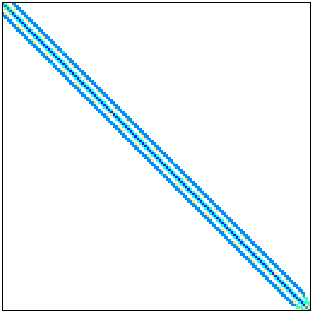
\includegraphics[width=.7\textwidth, keepaspectratio, clip]{Images/ch3/matrices/s1rmq4m1.png}
		\subcaption{s1rmq4m1}
		\label{Subfigure:benchmark-results-bandwidth-of-the-implementations-matrix-s1rmq4m1}
	\end{subfigure}%
	\begin{subfigure}{.5\textwidth}
		\centering
		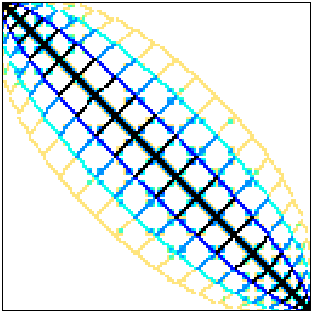
\includegraphics[width=.7\textwidth, keepaspectratio, clip]{Images/ch3/matrices/na5.png}
		\subcaption{Na5}
		\label{Subfigure:benchmark-results-bandwidth-of-the-implementations-matrix-na5}
	\end{subfigure}
	\caption{Nonzero element pattern of the \textit{s1rmq4m1} and \textit{Na5} matrices. Taken from the \emph{The university of Florida sparse matrix collection} \cite{Davis2011}.}
	\label{Figure:benchmark-results-bandwidth-of-the-implementations-matrices-s1rmq4m1-na5}
\end{figure}

As can be seen from Figure~\ref{Subfigure:benchmark-results-bandwidth-of-the-implementations-matrix-s1rmq4m1}, matrix \textit{s1rmq4m1} has nonzero elements on and near its main diagonal. Thus, the matrices arising from the decomposition ($ \mathbb{L} $ and $ \mathbb{U} $, or $ \mathbb{Z} $) will also have elements mainly around their main diagonals. From the perspective of ICM$ x $ this means that the majority of elements requiring computation are found within diagonal sections, therefore, more iterations are required to converge them. On the other hand, non-diagonal sections do not require as many iterations to converge as they contain mostly zeros. Consequently, ICM$ x $ is able to leverage the fact that each diagonal section has the device's resources available to itself and that non-diagonal sections converge in fewer iterations which results in a fast decomposition of the input matrix. In other words, ICM$ x $ is efficient at decomposing n-diagonal sparse matrices, i.e. matrices that have a small number (n) of nonzero diagonals near the main nonzero diagonal. For the \textit{s1rmq4m1} matrix - using either precision - the optimal number of threads per block is either $ 16 \times 16 $ or $ 32 \times 32 $. \\
Similarly, the \textit{Na5} matrix (Figure~\ref{Subfigure:benchmark-results-bandwidth-of-the-implementations-matrix-na5}) has more so an n-diagonal nonzero element structure with minor protrusions in the center. However, the protrusions do not impact the performance severely since the concentration of nonzero elements on the main diagonal is greater than that of the outer diagonals. Therefore, ICM$ x $ also benefits from the fact that, overall, fewer iterations are required to converge to an approximate solution.
\par Conversely, ICM$ x $ achieved its lowest bandwidth across all dense matrices when using double precision. Since the dense matrices used contain only nonzero elements, every section needed many iterations to be converged which in turn meant that, overall, more iterations were needed to converge the entire matrix. For context, the \textit{Cejka5943} dense matrix was decomposed by ICM32 in $ 44.53 $ seconds (using double precision), whereas the \textit{Na5} matrix was decomposed in $ 0.12 $ seconds. On the other hand, when single precision was used, the noticeable difference in performance between sparse and dense matrices was not as prominent. While the reason behind the stark performance difference between single and double precision for ICM$ x $ on dense matrices remains unproven, high-speed shared memory access and generally faster operations using single precision are suspected to be the root causes.
\par ICM$ x $ achieved higher bandwidths on all sparse matrix with the exception of the \textit{bcsstk03} (Figure~\ref{Subfigure:benchmark-results-bandwidth-of-the-implementations-matrix-bcsstk03}) and \textit{rail\_5177} (Figure~\ref{Subfigure:benchmark-results-bandwidth-of-the-implementations-matrix-rail_5177}) matrices despite the former's nonzero element structure being favorable to ICM$ x $. As Table~\ref{Table:benchmark-results-matrices-used-for-benchmarks-14-selected-matrices} lists, the dimensions of the \textit{bcsstk03} matrix are $ 112\times 112 $ which is advantageous for the sequential implementation of CM, as there are fewer steps to perform. Furthermore, since the matrix was already present in host memory, CM's decomposition procedure began without delay. On the other hand, for ICM$ x $, the matrix first had to be copied to device memory and, additionally, the pre-kernel overhead subroutine of ICM$ x $ took - in this case - relatively valuable time to complete. This, combined with the fact that the strength of the iterative algorithm lies in the GPU's ability to process larger datasets, indicates that CM is more suitable for decomposing smaller matrices. \\
When it comes to the \textit{rail\_5177} matrix (Figure~\ref{Subfigure:benchmark-results-bandwidth-of-the-implementations-matrix-rail_5177}), irrespective of the fact that its main diagonal is heavily populated with nonzero elements, there are other nonzero elements interspersed in a seemingly random fashion throughout the matrix. Therefore, similarly to dense matrices, the non-diagonal sections of this matrix also require more iterations to converge.

\begin{figure}[h!]
	\centering
	\begin{subfigure}{.5\textwidth}
		\centering
		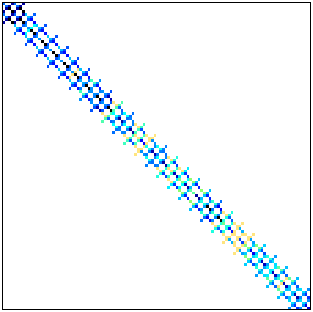
\includegraphics[width=.7\textwidth, keepaspectratio, clip]{Images/ch3/matrices/bcsstk03.png}
		\subcaption{bcsstk03}
		\label{Subfigure:benchmark-results-bandwidth-of-the-implementations-matrix-bcsstk03}
	\end{subfigure}%
	\begin{subfigure}{.5\textwidth}
		\centering
		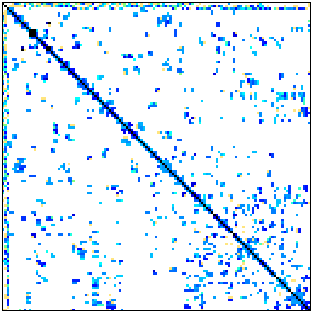
\includegraphics[width=.7\textwidth, keepaspectratio, clip]{images/ch3/matrices/rail_5177.png}
		\subcaption{rail\_5177}
		\label{Subfigure:benchmark-results-bandwidth-of-the-implementations-matrix-rail_5177}
	\end{subfigure}
	\caption{Nonzero element pattern of the \textit{bcsstk03} and \textit{rail\_5177} matrices. Taken from the \emph{The university of Florida sparse matrix collection} \cite{Davis2011}.}
	\label{Figure:benchmark-results-bandwidth-of-the-implementations-matrices-rail_5177-bcsstk03}
\end{figure}

The performance of ICM8 - as shown in Figure~\ref{Graph:benchmark-results-bandwidth-of-the-implementations-single-double-precision} - brings some interesting results. In general, its performance follows that of ICM16 and ICM32, however, some anomalous behavior is present in both single and double precision. For the former, bandwidths achieved seem to be slightly lower for the first $ 10 $ matrices (\textit{bcsstk03} to \textit{Cejka5943}), however, they are considerably lower the larger the matrix dimensions become. This behavior is most likely a result of global memory access becoming a greater bottleneck for single precision when decomposing larger matrices. Consequently, as non-coalesced global memory access is more common for ICM8 than for ICM16, or ICM32 (detailed further in Section~\ref{Subsection:benchmark-results-speedup-comparison-between-CM-and-different-ICMs}), its performance is proportionately lower. For double precision, ICM8 retains the relative performance difference compared to single precision. This is true even when it comes to the \textit{LeGresley\_2508} matrix (Figure~\ref{Figure:benchmark-results-bandwidth-of-the-implementations-matrix-legresley_2508}) which cannot be said about ICM16 and ICM32.

\begin{wrapfigure}{r}{.5\textwidth}
	\centering
	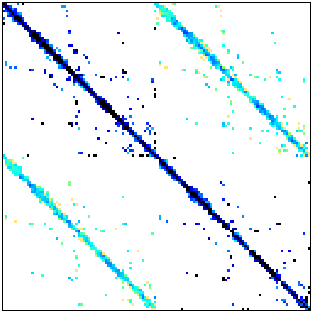
\includegraphics[width=.35\textwidth, keepaspectratio, clip]{images/ch3/matrices/legresley_2508.png}
	\caption{Nonzero element pattern of the \mbox{\textit{LeGresley\_2508}} matrix. Taken from the \emph{The university of Florida sparse matrix collection} \cite{Davis2011}.}
	\label{Figure:benchmark-results-bandwidth-of-the-implementations-matrix-legresley_2508}
\end{wrapfigure}

When comparing the differences in performance over all matrices between single and double precision for ICM16 and ICM32, the results seem consistent with the exception of certain dense matrices and the \textit{LeGresley\_2508} matrix (Figure~\ref{Figure:benchmark-results-bandwidth-of-the-implementations-matrix-legresley_2508}). When double precision is used, the performance of the mentioned implementations decreased drastically compared to single precision and compared to the decrease in performance of ICM8. Since $ 1/10 $ of the matrix dimensions are $ 250.8 $, \code{sectionSize} is set to \code{256} - the edge of the interval. Thus, \code{sectionSize} is the same for ICM8, ICM16, and ICM32 as their respective \code{BLOCK\_SIZE} is a divisor of \code{256}. Therefore, from the perspective of software, the only difference between the implementations in this instance - except for the precision - is the different \code{BLOCK\_SIZE}. It can be argued that ICM8 performed better due to the greater granularity of its thread blocks combined with the smaller size of the matrix. The greater granularity stems from the fact that ICM8 had $ 32 $ blocks assigned to each SM, whereas ICM16 had $ 8 $ and ICM32 had $ 2 $ - the A100 has a maximum of 2048 threads (64 warps; 32 blocks) per SM \cite{soj8qSRbfefUdi8Y}. This means that if the GPU would run out of resources in terms of concurrently active threads, then ICM8 would fair better as its smaller blocks could fill up the remaining resources more tightly (detailed in \textit{\nameref{Paragraph:CUDA-thread-management-grid}} in Section~\ref{Paragraph:CUDA-thread-management-grid}). This effect is only observed when decomposing smaller matrices which have a nonzero element structure similar to that of \textit{LeGresley\_2508}, i.e. matrices with nonzero elements on the main diagonal and nonzero elements interspersed elsewhere. Figure~\ref{Graph:benchmark-results-performance-of-implementations-across-all-matrices-bandwidth-double-precision} further confirms this suspicion for certain matrices where ICM8 outperforms ICM16 and ICM32 when double precision is used. For matrices with larger dimensions this effect would be mitigated since being able to utilize a few additional blocks would not amount to such a drastic difference in performance. Furthermore, the non-coalesced global memory access present for ICM8 (more so than ICM16) becomes apparent when decomposing larger matrices - especially when using single precision.
\par Other than the notable bandwidth achieved on the \textit{bcsstk03} matrix, in general, the performance of CM was lower than that of ICM$ x $ - especially when single precision was used. Conversely, when double precision was used, its performance on dense matrices was comparable to that of ICM$ x $. Specifically, the bandwidth achieved for matrices \textit{Cejka2842}, \textit{Cejka5943}, \textit{Cejka7580}, and \textit{Cejka10793} by CM and ICM32 (best ICM$ x $ for the matrices mentioned) can be seen in Table~\ref{Table:benchmark-results-bandwidth-of-the-implementations-dense-matrices-bandwidth}.

\begin{table}[h!]
	\centering
	\renewcommand{\arraystretch}{1.5}
	\begin{tabular}{ |c|c|c|c|c| } 
		\hline
		Implementation & Cejka2842 & Cejka5943 & Cejka7580 & Cejka10793 \\
		\hline
		CM             &     0.047 &     0.014 &     0.014 & 0.007      \\
		\hline
		ICM32          &     0.093 &     0.032 &     0.021 & 0.011      \\
		\hline
	\end{tabular}
	\caption{Bandwidth achieved (in GByte/s) when decomposing the subset of dense matrices from Table~\ref{Table:benchmark-results-matrices-used-for-benchmarks-14-selected-matrices} by CM and ICM32 using double precision.}
	\label{Table:benchmark-results-bandwidth-of-the-implementations-dense-matrices-bandwidth}
\end{table}

Since the algorithm used for CM is sequential and computes every element of the resulting decomposed matrix $ \mathbb{Z} $ regardless of its value, then there is no difference in how it computes matrices with distinct nonzero element structures. However, it can be argued that - especially when double precision is used - sparse matrices are, in general, decomposed slightly faster than dense matrices with the same dimensions. This is due to the fact that the multiplication and addition operations performed will be working with zeros in the majority of cases. Nevertheless, it can be concluded that the performance of CM is determined more so by the dimensions of a matrix, rather than its nonzero element structure.


\subsection{Speedup Comparison Between CM and different ICMs \TO}\label{Subsection:benchmark-results-speedup-comparison-between-CM-and-different-ICMs}
As the bandwidth results shown in Figure~\ref{Graph:benchmark-results-bandwidth-of-the-implementations-single-double-precision} are presented with a $ \log $-scaled vertical axis, it can be difficult to see the performance differences between implementations. Therefore, to put the results into perspective, this section presents the speedup comparison between the implementations listed in Section~\ref{Section:benchmark-results-benchmarked-implementations}. Specifically, as mentioned in \textit{\nameref{Paragraph:implementation-decomposition-project-lu-decomposition-implementation-requirements}} in Section~\ref{Paragraph:implementation-decomposition-project-lu-decomposition-implementation-requirements} one of the goals of this project was to "\textit{measure the acceleration of the GPU version of the LU decomposition against the CPU version}". For that reason, speedup from the CM (host) implementation to the ICM$ x $ (device) implementations will be compared. The comparison - using single and double precision - on the set of matrices listed in Table~\ref{Table:benchmark-results-matrices-used-for-benchmarks-14-selected-matrices} is shown in Figure~\ref{Graph:benchmark-results-speedup-comparison-between-CM-and-different-ICMs-single-double-precision}.

\begin{figure}[h!]
	\centering
	\tikzset{mark options={mark size=2.0, line width=0.5pt},font=\small}
	\begin{subfigure}{\textwidth}
		\begin{tikzpicture}
			\begin{axis}
				[
				,width=0.8\textwidth
				,height=0.45\textwidth
				,axis x line*=bottom
				,axis y line*=left
				,xlabel=\textbf{Matrix}
				,x label style={at={(axis description cs:0.575,-0.35)}}
				,ylabel=\textbf{Speedup}
				,xmin=-.5, xmax=13.5
				,ymin=-200, ymax=2100
				,xtick=data,
				,ytick={1, 500, 1000, 1500, 2000}
				,xticklabels={bcsstk03,494\_bus,LeGresley\_2508,Cejka2842,rail\_5177,c-31,s3rmt3m3,s1rmq4m1,Na5,Cejka5943,fp,Cejka7580,bundle1,Cejka10793}
				,x tick label style={rotate=45,anchor=east,yshift=-6pt,align=right}
				,ymajorgrids
				,legend pos=outer north east
				]
				\addplot[black,mark=triangle*] table [x=id, y=cm-speedup, col sep=comma] {resources/plot-csv-files/14-matrices-single-precision-rci.csv};
				\addplot[red,mark=x] table [x=id, y=icm8-speedup, col sep=comma] {resources/plot-csv-files/14-matrices-single-precision-rci.csv};
				\addplot[green!60!black,mark=square*] table [x=id, y=icm16-speedup, col sep=comma] {resources/plot-csv-files/14-matrices-single-precision-rci.csv};
				\addplot[blue,mark=triangle*] table [x=id, y=icm32-speedup, col sep=comma] {resources/plot-csv-files/14-matrices-single-precision-rci.csv};
				\legend{CM, ICM8, ICM16, ICM32}
			\end{axis}
		\end{tikzpicture}
		\subcaption{Single precision}
		\label{Graph:benchmark-results-speedup-comparison-between-CM-and-different-ICMs-single-precision}
	\end{subfigure}
	\begin{subfigure}{\textwidth}
		\begin{tikzpicture}
			\begin{axis}
				[
				,width=0.8\textwidth
				,height=0.45\textwidth
				,axis x line*=bottom
				,axis y line*=left
				,xlabel=\textbf{Matrix}
				,x label style={at={(axis description cs:0.575,-0.35)}}
				,ylabel=\textbf{Speedup}
				,xmin=-.5, xmax=13.5
				,ymin=-200, ymax=2100
				,ytick={1, 500, 1000, 1500, 2000}
				,xtick=data,
				,xticklabels={bcsstk03,494\_bus,LeGresley\_2508,Cejka2842,rail\_5177,c-31,s3rmt3m3,s1rmq4m1,Na5,Cejka5943,fp,Cejka7580,bundle1,Cejka10793}
				,x tick label style={rotate=45,anchor=east,yshift=-6pt,align=right}
				,ymajorgrids
				,legend pos=outer north east
				]
				\addplot[black,mark=triangle*] table [x=id, y=cm-speedup, col sep=comma] {resources/plot-csv-files/14-matrices-double-precision-rci.csv};
				\addplot[red,mark=x] table [x=id, y=icm8-speedup, col sep=comma] {resources/plot-csv-files/14-matrices-double-precision-rci.csv};
				\addplot[green!60!black,mark=square*] table [x=id, y=icm16-speedup, col sep=comma] {resources/plot-csv-files/14-matrices-double-precision-rci.csv};
				\addplot[blue,mark=triangle*] table [x=id, y=icm32-speedup, col sep=comma] {resources/plot-csv-files/14-matrices-double-precision-rci.csv};
				\legend{CM, ICM8, ICM16, ICM32}
			\end{axis}
		\end{tikzpicture}
		\subcaption{Double precision}
	\end{subfigure}
	\caption{Speedup comparison between the decomposition times of CM and the ICM$ x $ implementations on the set of matrices (Table~\ref{Table:benchmark-results-matrices-used-for-benchmarks-14-selected-matrices}) using single and double precision. }
	\label{Graph:benchmark-results-speedup-comparison-between-CM-and-different-ICMs-single-double-precision}
\end{figure}

\paragraph{ICM16 and ICM32} Similarly to the bandwidth results, overall, ICM16 and ICM32 were the best-performing implementations. For single precision, the three highest speedups compared to CM were $ 2030.30 $ by ICM32 and $ 1803.08 $ by ICM16 on the \textit{bundle1} matrix (Figure~\ref{Subfigure:benchmark-results-speedup-comparison-between-CM-and-different-ICMs-matrix-bundle1}), and $ 1352.55 $ by ICM16 on the \textit{s1rmq4m1} matrix (Figure~\ref{Subfigure:benchmark-results-bandwidth-of-the-implementations-matrix-s1rmq4m1}). In terms of double precision, the highest speedups compared to CM were $ 1337.53 $ and $ 1137.98 $ achieved by ICM32 on matrices \textit{bundle1} and \textit{s1rmq4m1} respectively, and $ 1022.01 $ achieved by ICM16 on the \textit{bundle1} matrix.

\begin{figure}[h!]
	\centering
	\begin{subfigure}{.5\textwidth}
		\centering
		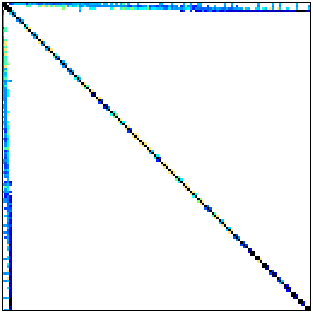
\includegraphics[width=.7\textwidth, keepaspectratio, clip]{Images/ch3/matrices/bundle1.png}
		\subcaption{bundle1}
		\label{Subfigure:benchmark-results-speedup-comparison-between-CM-and-different-ICMs-matrix-bundle1}
	\end{subfigure}%
	\begin{subfigure}{.5\textwidth}
		\centering
		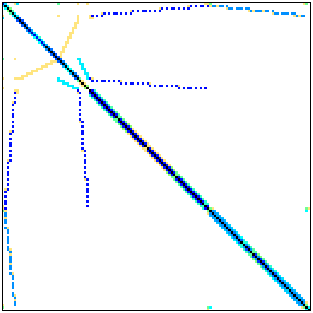
\includegraphics[width=.7\textwidth, keepaspectratio, clip]{images/ch3/matrices/s3rmt3m3.png}
		\subcaption{s3rmt3m3}
		\label{Subfigure:benchmark-results-speedup-comparison-between-CM-and-different-ICMs-matrix-s3rmt3m3}
	\end{subfigure}
	\caption{Nonzero element pattern of the \textit{bundle1} and \textit{s3rmt3m3} matrices. Taken from the \emph{The university of Florida sparse matrix collection} \cite{Davis2011}.}
	\label{Figure:benchmark-results-speedup-comparison-between-CM-and-different-ICMs-matrices-rail_5177-bcsstk03}
\end{figure}

Nevertheless, there are exceptions to the greater performance of ICM32. One such exception is the speedup compared to ICM8 on the \textit{s3rmt3m3} matrix (Figure~\ref{Subfigure:benchmark-results-speedup-comparison-between-CM-and-different-ICMs-matrix-s3rmt3m3}) when single precision is used. For this matrix, ICM32 achieved a speedup of $ 368.14 $, whereas ICM8 achieved $ 427.55 $. As can be seen from Figure~\ref{Subfigure:benchmark-results-speedup-comparison-between-CM-and-different-ICMs-matrix-s3rmt3m3} the nonzero element structure of the \textit{s3rmt3m3} matrix comprises of a strong concentration of nonzero elements along the main diagonal and six nonzero-element lines aimed away from the main diagonal. The reason mentioned for the higher performance on the \textit{Na5} matrix describes that a matrix with a similar nonzero element structure should not require many iterations to decompose for ICM$ x $ as the main diagonal has most of the nonzero elements and only a few other nonzero elements are found outside it. However, since the nonzero elements found outside the main diagonal are located much further from it than that of the \textit{Na5} matrix pictured in Figure~\ref{Subfigure:benchmark-results-bandwidth-of-the-implementations-matrix-na5}, then the non-diagonal sections needed more iterations to converge.
\par Another noteworthy sparse matrix on which ICM$ x $ struggled - relative to the rest - was the \textit{fp} matrix (Figure~\ref{Figure:benchmark-results-speedup-comparison-between-CM-and-different-ICMs-matrix-fp}). It can be seen that the nonzero element structure is similar to that of the \textit{rail\_5177} matrix (Figure~\ref{Subfigure:benchmark-results-bandwidth-of-the-implementations-matrix-rail_5177}). In other words, nonzero elements are concentrated on the main diagonal and other nonzero elements are interspersed throughout the rest of the matrix. Consequently, the lack of performance by ICM$ x $ is due to more iterations required to converge the non-diagonal sections.

\begin{figure}[h!]
	\centering
	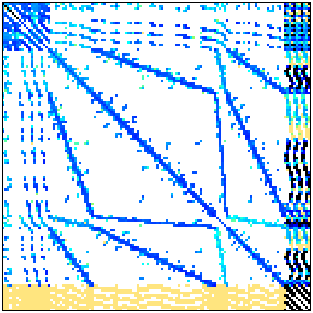
\includegraphics[width=.35\textwidth, keepaspectratio, clip]{images/ch3/matrices/fp.png}
	\caption{Nonzero element pattern of the \mbox{\textit{fp}} matrix. Taken from the \emph{The university of Florida sparse matrix collection} \cite{Davis2011}.}
	\label{Figure:benchmark-results-speedup-comparison-between-CM-and-different-ICMs-matrix-fp}
\end{figure}

\paragraph{ICM8} In general, ICM8 was faster than CM, however, when its speedup is compared to that of ICM16 and ICM32, there is a difference in performance. This difference is noticeable especially for matrices that required few iterations to decompose the entire matrix, for example, \textit{s1rmq4m1}, \textit{Na5}, and \textit{bundle1}. Since the decomposition time for these matrices was - at worst - $ 0.9 $ seconds for each, loading elements from global to shared memory became a bottleneck. The reason behind this stems from the fact that threads in blocks are divided into warps by their \code{threadIdx.x} index. Thus, when reading from shared memory threads in a warp should - ideally - access neighboring global memory addresses. Since elements of the \code{DenseMatrix} instance are stored in row-major order on the GPU, each warp in ICM8 loads elements from global memory in the following way: first 8 threads of the warp read data from neighboring addresses, the next 8 threads of the warp also read from other neighboring addresses, in other words, they are not found near the first 8 addresses (unless the matrix dimensions are $ 8\times 8 $) - this is non-coalesced access to memory. In this instance, the non-coalesced access is the same as depicted in the upper image of Figure~\ref{Sub-figure:CUDA-global-memory-non-coalesced-access-2}. Therefore, as mentioned in the figure's caption, instead of the threads in a warp performing one transaction to global memory, they will perform $ 32/8 = 4 $ sequential transactions (detailed further in \textit{\nameref{Paragraph:CUDA-memory-management-global-memory}} in Section~\ref{Paragraph:CUDA-memory-management-global-memory}). \\
This means that non-coalesced access to global memory occurs for ICM8 and ICM16, however, the latter will only perform $ 32/16 = 2 $ sequential transactions. On the other hand, this defect is not present for ICM32 as the threads of a warp access \code{BLOCK\_SIZE = 32} neighboring addresses in global memory. This effect is apparent in Figure~\ref{Graph:benchmark-results-speedup-comparison-between-CM-and-different-ICMs-single-double-precision} (ICM32 performed better than ICM16 which outperformed ICM8), especially when decomposing the previously-mentioned matrices: \textit{s1rmq4m1}, \textit{Na5} and \textit{bundle1} using double precision.
\paragraph{CM}\label{Paragraph:benchmark-results-speedup-comparison-between-CM-and-different-ICMs-CM-speedup-description}
In Figure~\ref{Graph:benchmark-results-speedup-comparison-between-CM-and-different-ICMs-single-double-precision} it can be seen that CM took more time to decompose most of the benchmarked matrices. However, an interesting result arises when comparing CM and ICM8 for double precision. Specifically, for $ 3 $ out of the $ 14 $ matrices, ICM8 was slower than CM as it achieved the following speedups: $ 0.09 $ for \textit{bcsstk03}, $ 0.92 $ for \textit{Cejka7580}, and $ 0.96 $ for \textit{Cejka10793}. While the result for \textit{bcsstk03} is not surprising given the matrix's dimensions, the others are. The most likely reason for the lower performance is the non-coalesced access to global memory which is most prominent for ICM8.
\par Overall, the decomposition of matrices using single precision was faster compared to double precision. However, the difference in speed is not clearly visible from either Figure~\ref{Graph:benchmark-results-bandwidth-of-the-implementations-single-double-precision} (due to the vertical axis being $ \log $-scaled) or Figure~\ref{Graph:benchmark-results-speedup-comparison-between-CM-and-different-ICMs-single-double-precision} (due to the range of the speedup factor being too great for the values to be distinguishable). For this reason, the raw execution times for single and double precision are included in Table~\ref{Table:benchmark-results-speedup-comparison-between-CM-and-different-ICMs-execution-times-single-precision} and Table~\ref{Table:benchmark-results-speedup-comparison-between-CM-and-different-ICMs-execution-times-double-precision} respectively.

\begin{table}[h!]
	\centering
	\begin{tabular}{|>{\footnotesize}l|>{\raggedleft\arraybackslash\footnotesize}r|>{\raggedleft\arraybackslash\footnotesize}r|>{\raggedleft\arraybackslash\footnotesize}r|>{\raggedleft\arraybackslash\footnotesize}r|}
		\hline
		\multicolumn{1}{|>{\centering\footnotesize}c|}{Matrix} & \multicolumn{1}{>{\centering\footnotesize}c|}{CM} & \multicolumn{1}{>{\centering\footnotesize}c|}{ICM8} & \multicolumn{1}{>{\centering\footnotesize}c|}{ICM16} & \multicolumn{1}{>{\centering\footnotesize}c|}{ICM32} \\ \hline
		bcsstk03        & \cellcolor{green!25}0.0002 &  0.0022 &                     0.0020 &                     0.0022 \\
		494\_bus 		&                     0.0292 &  0.0049 &                     0.0053 & \cellcolor{green!25}0.0043 \\
		LeGresley\_2508 &                     4.2193 &  0.0793 & \cellcolor{green!25}0.0498 &                     0.0531 \\
		Cejka2842		&                     6.2210 &  3.0391 & \cellcolor{green!25}2.1182 &                     2.1412 \\
		rail\_5177      &                    55.1124 &  1.4350 & \cellcolor{green!25}1.0669 &                     1.1022 \\
		c-31		    &                    59.3208 &  0.1598 &                     0.1330 & \cellcolor{green!25}0.1327 \\
		s3rmt3m3        &                    61.9867 &  0.1450 & \cellcolor{green!25}0.1133 &                     0.1684 \\
		s1rmq4m1        &                    67.8509 &  0.0641 & \cellcolor{green!25}0.0502 &                     0.0505 \\
		Na5             &                    62.3995 &  0.0817 & \cellcolor{green!25}0.0636 &                     0.0649 \\
		Cejka5943		&                    90.1114 &  0.7035 &                     0.5230 & \cellcolor{green!25}0.4856 \\
		fp              &                   179.7054 &  0.5278 &                     0.3980 & \cellcolor{green!25}0.3690 \\
		Cejka7580		&                   151.7981 & 12.2164 &                     3.0289 & \cellcolor{green!25}2.2853 \\
		bundle1         &                   617.5120 &  0.4853 &                     0.3425 & \cellcolor{green!25}0.3041 \\
		Cejka10793      &                   643.3462 &  9.2837 &                     2.8510 & \cellcolor{green!25}2.2107 \\ \hline
	\end{tabular}
	\caption{The execution time (in seconds) of decomposition for all implementations on the set of matrices (Table~\ref{Table:benchmark-results-matrices-used-for-benchmarks-14-selected-matrices}) using \textbf{single} precision. The fastest time for each matrix is highlighted in green.}
	\label{Table:benchmark-results-speedup-comparison-between-CM-and-different-ICMs-execution-times-single-precision}
\end{table}

\begin{table}[h!]
	\centering
	\begin{tabular}{|>{\footnotesize}l|>{\raggedleft\arraybackslash\footnotesize}r|>{\raggedleft\arraybackslash\footnotesize}r|>{\raggedleft\arraybackslash\footnotesize}r|>{\raggedleft\arraybackslash\footnotesize}r|}
		\hline
		\multicolumn{1}{|>{\centering\footnotesize}c|}{Matrix} & \multicolumn{1}{>{\centering\footnotesize}c|}{CM} & \multicolumn{1}{>{\centering\footnotesize}c|}{ICM8} & \multicolumn{1}{>{\centering\footnotesize}c|}{ICM16} & \multicolumn{1}{>{\centering\footnotesize}c|}{ICM32} \\ \hline
		bcsstk03        & \cellcolor{green!25}0.0003 &                     0.0027 &                     0.0026 &                       0.0027 \\
		494\_bus 		&                     0.0299 &                     0.0084 & \cellcolor{green!25}0.0070 &                       0.0082 \\
		LeGresley\_2508 &                     4.3542 & \cellcolor{green!25}0.2055 &                     0.4805 &                       0.6118 \\
		Cejka2842		&                     6.9110 &                     4.5995 &                     3.6436 & \cellcolor{green!25}  3.4559 \\
		rail\_5177      &                    67.9030 &                     3.0109 &                     2.3882 & \cellcolor{green!25}  2.1754 \\
		c-31		    &                    72.3863 &                     0.4913 &                     0.4166 & \cellcolor{green!25}  0.3349 \\
		s3rmt3m3        &                    74.0106 &                     0.3704 &                     0.2997 & \cellcolor{green!25}  0.2577 \\
		s1rmq4m1        &                    81.2749 &                     0.1059 &                     0.0843 & \cellcolor{green!25}  0.0714 \\
		Na5             &                    67.2166 &                     0.1543 &                     0.1365 & \cellcolor{green!25}  0.1243 \\
		Cejka5943		&                   104.6150 &                    70.8865 &                    56.2768 & \cellcolor{green!25} 44.5275 \\
		fp              &                   154.8232 &                     0.9641 &                     0.7715 & \cellcolor{green!25}  0.6287 \\
		Cejka7580		&                   159.6421 &                   172.9549 &                   138.9242 & \cellcolor{green!25}107.8041 \\
		bundle1         &                   679.3846 &                     0.8859 &                     0.6648 & \cellcolor{green!25}  0.5079 \\
		Cejka10793      &                   699.9634 &                   731.9412 &                   556.0243 & \cellcolor{green!25}419.1401 \\ \hline
	\end{tabular}
	\caption{The execution time (in seconds) of decomposition for all implementations on the set of matrices (Table~\ref{Table:benchmark-results-matrices-used-for-benchmarks-14-selected-matrices}) using \textbf{double} precision. The fastest time for each matrix is highlighted in green.}
	\label{Table:benchmark-results-speedup-comparison-between-CM-and-different-ICMs-execution-times-double-precision}
\end{table}

From the results presented in Table~\ref{Table:benchmark-results-speedup-comparison-between-CM-and-different-ICMs-execution-times-single-precision} it could be concluded that ICM32 is the most suitable implementation for decomposing matrices using single precision. In terms of double precision the same statement could be made when looking at Table~\ref{Table:benchmark-results-speedup-comparison-between-CM-and-different-ICMs-execution-times-double-precision}. However, since the results presented in the mentioned tables were only a small subset of all results, verification of this claim is required for the entire set of $ 63 $ matrices.

\subsection{Performance of Implementations Across All Matrices \TO}\label{Subsection:benchmark-results-performance-of-implementations-across-all-matrices}
This section shows the bandwidth, speedup comparison, and accuracy of results - using both single and double precision - for the decomposition implementations listed in Section~\ref{Section:benchmark-results-benchmarked-implementations}. The metrics were measured across the entire set of 63 matrices and the benchmarks were run on the platform specified in Table~\ref{Table:benchmark-results-benchmark-platform-specifications}. In order to illustrate how ICM$ x $ compares to CM on matrices that increase in size, the matrices in the graphs were sorted from smallest to largest. The bandwidth results can be found in Figure~\ref{Graph:benchmark-results-performance-of-implementations-across-all-matrices-bandwidth-single-double-precision}, the speedup comparison between CM and ICM$ x $ can be found in Figure~\ref{Graph:benchmark-results-performance-of-implementations-across-all-matrices-speedup-single-double-precision}, and the accuracy of the results can be found in Figure~\ref{Graph:benchmark-results-performance-of-implementations-across-all-matrices-accuracy-single-double-precision}. All figures in this section have a $ \log $-scaled vertical axis as the range of values was too great to present any coherent data.

\paragraph{Bandwidth} As shown in Figure~\ref{Graph:benchmark-results-performance-of-implementations-across-all-matrices-bandwidth-single-double-precision}, in terms of bandwidth, the ICM$ x $ implementations achieved similar results with the exception of ICM8 that is noticeably less performant. The lack of ICM8's performance is more prominent for single precision where the issue with non-coalesced global memory access appears to be making a difference. This is further supported by the fact that after a certain point (matrix $ 46 $) ICM8 appears to be consistently falling behind ICM32 in terms of bandwidth achieved - especially noticeable for the larger dense matrices (the three dips in bandwidth after matrix $ 55 $ in Figure~\ref{Graph:benchmark-results-performance-of-implementations-across-all-matrices-bandwidth-single-precision}).
\par In terms of double precision the performance of ICM$ x $ is more consistent. The general rule of ICM8 performing worse than ICM16 and ICM32 for larger matrices still stands and the performance of ICM16 for matrices past matrix $ 30 $ is - in the majority of cases - less than that of ICM32. The dips in bandwidth of ICM$ x $ for matrices past matrix $ 25 $ are caused by the dense matrices found in the set. For the majority of matrices, the bandwidth achieved during their decomposition was greater than 1 GByte/s for both single and double precision. On the other hand, Figure~\ref{Graph:benchmark-results-performance-of-implementations-across-all-matrices-bandwidth-single-double-precision} shows that the bandwidth achieved by CM decreases in an almost logarithmic fashion with increasing matrix dimensions.
\par Contrary to what the subset of results presented in Section~\ref{Subsection:benchmark-results-bandwidth-of-the-implementations} seemed to suggest, it can be seen from Figure~\ref{Graph:benchmark-results-performance-of-implementations-across-all-matrices-bandwidth-single-precision} (single precision) and Figure~\ref{Graph:benchmark-results-performance-of-implementations-across-all-matrices-bandwidth-double-precision} (double precision) that CM outperformed ICM$ x $ in more cases than just one. Although, it must be mentioned that the matrices on which CM achieved a higher bandwidth than ICM$ x $ did have dimensions between $ 27\times 27 $ and $ 415\times 415 $.

\begin{figure}[h!]
	\centering
	\tikzset{mark options={mark size=1.5},font=\small}
	\begin{subfigure}{\textwidth}
		\begin{tikzpicture}
			\begin{axis}
				[
				,width=\textwidth
				,height=0.45\textwidth
				,axis x line*=bottom
				,axis y line*=left
				,xlabel=\textbf{Matrix ID}
				,ylabel=\textbf{GByte/s} ($ \log $ scale)
				,x label style={at={(axis description cs:0.46,-.1)}}
				,xmin=-1, xmax=63
				,ymode=log
				,ymajorgrids
				,legend style={at={(0.5,1.15)},anchor=north,cells={anchor=east},legend columns=-1}
				]
				\addplot[black,mark=*] table [x=id, y=cm-bandwidth, col sep=comma] {resources/plot-csv-files/63-matrices-single-precision-rci.csv};
				\addplot[red,mark=*] table [x=id, y=icm8-bandwidth, col sep=comma] {resources/plot-csv-files/63-matrices-single-precision-rci.csv};
				\addplot[green!60!black,mark=*] table [x=id, y=icm16-bandwidth, col sep=comma] {resources/plot-csv-files/63-matrices-single-precision-rci.csv};
				\addplot[blue,mark=*] table [x=id, y=icm32-bandwidth, col sep=comma] {resources/plot-csv-files/63-matrices-single-precision-rci.csv};
				\legend{CM, ICM8, ICM16, ICM32}
			\end{axis}
		\end{tikzpicture}
		\subcaption{Single precision}
		\label{Graph:benchmark-results-performance-of-implementations-across-all-matrices-bandwidth-single-precision}
	\end{subfigure}
	\vspace{0.25cm}
	\begin{subfigure}{\textwidth}
		\begin{tikzpicture}
			\begin{axis}
				[
				,width=\textwidth
				,height=0.45\textwidth
				,axis x line*=bottom
				,axis y line*=left
				,xlabel=\textbf{Matrix ID}
				,ylabel=\textbf{GByte/s} ($ \log $ scale)
				,x label style={at={(axis description cs:0.46,-.1)}}
				,xmin=-1, xmax=63
				,ymode=log
				,ymajorgrids
				,legend style={at={(0.5,1.15)},anchor=north,cells={anchor=east},legend columns=-1}
				]
				\addplot[black,mark=*] table [x=id, y=cm-bandwidth, col sep=comma] {resources/plot-csv-files/63-matrices-double-precision-rci.csv};
				\addplot[red,mark=*] table [x=id, y=icm8-bandwidth, col sep=comma] {resources/plot-csv-files/63-matrices-double-precision-rci.csv};
				\addplot[green!60!black,mark=*] table [x=id, y=icm16-bandwidth, col sep=comma] {resources/plot-csv-files/63-matrices-double-precision-rci.csv};
				\addplot[blue,mark=*] table [x=id, y=icm32-bandwidth, col sep=comma] {resources/plot-csv-files/63-matrices-double-precision-rci.csv};
				\legend{CM, ICM8, ICM16, ICM32}
			\end{axis}
		\end{tikzpicture}
		\subcaption{Double precision}
		\label{Graph:benchmark-results-performance-of-implementations-across-all-matrices-bandwidth-double-precision}
	\end{subfigure}
	\caption{Bandwidths achieved by decomposition implementations listed in Section~\ref{Section:benchmark-results-benchmarked-implementations} on the entire set of $ 63 $ matrices using both single and double precision. Matrix ID signifies the ID of the matrices, after they have been sorted according to their dimension from smallest to largest. The vertical axis is $ \log $-scaled for better visibility of differences between implementations.}
	\label{Graph:benchmark-results-performance-of-implementations-across-all-matrices-bandwidth-single-double-precision}
\end{figure}

\paragraph{Speedup} The speedup comparison in Figure~\ref{Graph:benchmark-results-performance-of-implementations-across-all-matrices-speedup-single-double-precision} is presented for the sake of completeness and to show how much faster the ICM$ x $ implementations were compared to CM. Specifically, when single precision was used, all ICM$ x $ implementations were faster in $ 54/63 $ cases. In terms of double precision, ICM8 was faster in $ 51/63 $ cases, and ICM32 and ICM16 were faster in $ 53/63 $. However, as mentioned before, all of the matrices (with the two exceptions for ICM8 detailed in \textit{\nameref{Paragraph:benchmark-results-speedup-comparison-between-CM-and-different-ICMs-CM-speedup-description}} in Section~\ref{Paragraph:benchmark-results-speedup-comparison-between-CM-and-different-ICMs-CM-speedup-description}) that CM decomposed faster than ICM$ x $ have dimensions $ 415\times 415 $ or smaller.

\begin{figure}[h!]
	\centering
	\tikzset{mark options={mark size=1.5},font=\small}
	\begin{subfigure}{\textwidth}
		\begin{tikzpicture}
			\begin{axis}
				[
				,width=\textwidth
				,height=0.45\textwidth
				,axis x line*=bottom
				,axis y line*=left
				,xlabel=\textbf{Matrix ID}
				,ylabel=\textbf{Speedup} ($ \log $ scale)
				,x label style={at={(axis description cs:0.46,-.1)}}
				,xmin=-1, xmax=63
				,ymode=log
				,ymajorgrids
				,legend style={at={(0.5,1.15)},anchor=north,cells={anchor=east},legend columns=-1}
				]
				\addplot[black,mark=*] table [x=id, y=cm-speedup, col sep=comma] {resources/plot-csv-files/63-matrices-single-precision-rci.csv};
				\addplot[red,mark=*] table [x=id, y=icm8-speedup, col sep=comma] {resources/plot-csv-files/63-matrices-single-precision-rci.csv};
				\addplot[green!60!black,mark=*] table [x=id, y=icm16-speedup, col sep=comma] {resources/plot-csv-files/63-matrices-single-precision-rci.csv};
				\addplot[blue,mark=*] table [x=id, y=icm32-speedup, col sep=comma] {resources/plot-csv-files/63-matrices-single-precision-rci.csv};
				\legend{CM, ICM8, ICM16, ICM32}
			\end{axis}
		\end{tikzpicture}
		\subcaption{Single precision}
		\label{Graph:benchmark-results-performance-of-implementations-across-all-matrices-speedup-single-precision}
	\end{subfigure}
	\vspace{0.25cm}
	\begin{subfigure}{\textwidth}
		\begin{tikzpicture}
			\begin{axis}
				[
				,width=\textwidth
				,height=0.45\textwidth
				,axis x line*=bottom
				,axis y line*=left
				,xlabel=\textbf{Matrix ID}
				,ylabel=\textbf{Speedup} ($ \log $ scale)
				,x label style={at={(axis description cs:0.46,-.1)}}
				,xmin=-1, xmax=63
				,ymode=log
				,ymajorgrids
				,legend style={at={(0.5,1.15)},anchor=north,cells={anchor=east},legend columns=-1}
				]
				\addplot[black,mark=*] table [x=id, y=cm-speedup, col sep=comma] {resources/plot-csv-files/63-matrices-double-precision-rci.csv};
				\addplot[red,mark=*] table [x=id, y=icm8-speedup, col sep=comma] {resources/plot-csv-files/63-matrices-double-precision-rci.csv};
				\addplot[green!60!black,mark=*] table [x=id, y=icm16-speedup, col sep=comma] {resources/plot-csv-files/63-matrices-double-precision-rci.csv};
				\addplot[blue,mark=*] table [x=id, y=icm32-speedup, col sep=comma] {resources/plot-csv-files/63-matrices-double-precision-rci.csv};
				\legend{CM, ICM8, ICM16, ICM32}
			\end{axis}
		\end{tikzpicture}
		\subcaption{Double precision}
		\label{Graph:benchmark-results-performance-of-implementations-across-all-matrices-speedup-double-precision}
	\end{subfigure}
	\caption{Speedup comparison between CM and ICM$ x $ implementations on the entire set of $ 63 $ matrices using both single and double precision. Matrix ID signifies the ID of the matrices, after they have been sorted according to their dimension from smallest to largest. The vertical axis is $ \log $-scaled for better visibility of differences between implementations.}
	\label{Graph:benchmark-results-performance-of-implementations-across-all-matrices-speedup-single-double-precision}
\end{figure}

Additionally, Table~\ref{Table:benchmark-results-performance-of-implementations-across-all-matrices-total-execution-time-single-double-precision} shows the total time required by each implementation to decompose the set of $ 63 $ matrices using both single and double precision. The data in this table provides further support to the claim made at the end of Section~\ref{Subsection:benchmark-results-speedup-comparison-between-CM-and-different-ICMs} which stated that ICM32 is the most suitable implementation for single and double precision.

\begin{table}[h!]
	\centering
	\renewcommand{\arraystretch}{1.5}
	\begin{tabular}{|>{\footnotesize}l|>{\raggedleft\arraybackslash\footnotesize}r|>{\raggedleft\arraybackslash\footnotesize}r|>{\raggedleft\arraybackslash\footnotesize}r|>{\raggedleft\arraybackslash\footnotesize}r|}
		\hline
		\multicolumn{1}{|>{\centering\footnotesize}c|}{Matrix} & \multicolumn{1}{>{\centering\footnotesize}c|}{CM} & \multicolumn{1}{>{\centering\footnotesize}c|}{ICM8} & \multicolumn{1}{>{\centering\footnotesize}c|}{ICM16} & \multicolumn{1}{>{\centering\footnotesize}c|}{ICM32} \\ \hline
		Single        & 2393.09 &   35.88 &  17.36 & \cellcolor{green!25} 13.84 \\
		Double 		  & 2635.45 & 1000.27 & 772.29 & \cellcolor{green!25}592.19 \\ \hline
	\end{tabular}
	\caption{The total execution time (in seconds) taken by each implementation to decompose the set of $ 63 $ matrices (Table~\ref{Table:benchmark-results-matrices-used-for-benchmarks-14-selected-matrices}) on the RCI compute cluster specified in Table~\ref{Table:benchmark-results-benchmark-platform-specifications} using single and double precision. The fastest time for each precision is highlighted in green.}
	\label{Table:benchmark-results-performance-of-implementations-across-all-matrices-total-execution-time-single-double-precision}
\end{table}

\paragraph{Accuracy of results} While this part is the other key factor of the implementation (the first being speed of execution), it serves more as a means to verify that the presented performance does not come at the cost of drastically inaccurate results. Figure~\ref{Graph:benchmark-results-performance-of-implementations-across-all-matrices-accuracy-single-double-precision} shows the maximum difference between the input matrix $ \mathbb{A} $ and the multiplication of the decomposed matrices ($ \mathbb{L} $ and $ \mathbb{U} $, or $ \mathbb{Z} $), i.e.

\begin{equation}
	\max\left| \mathbb{A} - \mathbb{L}\mathbb{U}\right| \nonumber \,.
\end{equation}

In other words, the matrix that results from multiplying the matrices obtained from the decomposition ($ \mathbb{L} $ and $ \mathbb{U} $) should - ideally - be the same as the input matrix ($ \mathbb{A} $). The values presented in this part are the largest differences between the actual results and the ideal results.
\par For the purpose of this project, the maximum difference will also be referred to as the \textit{error}. Similarly to the previous figures, the vertical axis is $ \log $-scaled in order to present the results more clearly. This is due the fact that the data ranged from $ 268,435,500 $ to $ 0 $ for single precision and the median of the values for double precision was $ 2.32831\times10^{-10} $ with the data ranging from $ 2 $ to $ 0 $. The figure only shows data for ICM$ x $ as the accuracy of the results did not differ for the ICM$ x $ implementations.

\begin{figure}[h!]
	\centering
	\tikzset{mark options={mark size=1.5},font=\small}
	\begin{subfigure}{\textwidth}
		\begin{tikzpicture}
			\begin{axis}
				[
				,width=\textwidth
				,height=0.45\textwidth
				,axis x line*=bottom
				,axis y line*=left
				,xlabel=\textbf{Matrix ID}
				,ylabel=\textbf{Max. difference} ($ \log $ scale)
				,x label style={at={(axis description cs:0.46,-.1)}}
				,xmin=-1, xmax=63
				,ymode=log
				,ymajorgrids
				,legend style={at={(0.5,1.15)},anchor=north,cells={anchor=east},legend columns=-1}
				]
				\addplot[black,mark=*] table [x=id, y=cm-Adiff, col sep=comma] {resources/plot-csv-files/63-matrices-single-precision-rci.csv};
				\addplot[red,mark=*] table [x=id, y=icmx-Adiff, col sep=comma] {resources/plot-csv-files/63-matrices-single-precision-rci.csv};
				\legend{CM, ICM$ x $}
			\end{axis}
		\end{tikzpicture}
		\subcaption{Single precision}
		\label{Graph:benchmark-results-performance-of-implementations-across-all-matrices-accuracy-single-precision}
	\end{subfigure}
	\vspace{0.25cm}
	\begin{subfigure}{\textwidth}
		\begin{tikzpicture}
			\begin{axis}
				[
				,width=\textwidth
				,height=0.45\textwidth
				,axis x line*=bottom
				,axis y line*=left
				,xlabel=\textbf{Matrix ID}
				,ylabel=\textbf{Max. difference} ($ \log $ scale)
				,x label style={at={(axis description cs:0.46,-.1)}}
				,xmin=-1, xmax=63
				,ymode=log
				,ymajorgrids
				,legend style={at={(0.5,1.15)},anchor=north,cells={anchor=east},legend columns=-1}
				]
				\addplot[black,mark=*] table [x=id, y=cm-Adiff, col sep=comma] {resources/plot-csv-files/63-matrices-double-precision-rci.csv};
				\addplot[red,mark=*] table [x=id, y=icmx-Adiff, col sep=comma] {resources/plot-csv-files/63-matrices-double-precision-rci.csv};
				\legend{CM, ICM$ x $}
			\end{axis}
		\end{tikzpicture}
		\subcaption{Double precision}
		\label{Graph:benchmark-results-performance-of-implementations-across-all-matrices-accuracy-double-precision}
	\end{subfigure}
	\caption{Comparison of the accuracy of results between CM and ICM$ x $ implementations on the entire set of $ 63 $ matrices using both single and double precision. In this instance "\textit{accuracy}" refers to the maximum difference of $ \left| \mathbb{A} - \mathbb{L}\mathbb{U} \right| $ where $ \mathbb{A} $ is the input matrix and $ \mathbb{L} $ and $ \mathbb{U} $ are the matrices obtained from the decomposition procedure. The higher the maximum difference, the lower the accuracy of the results (the higher the error). Matrix ID signifies the ID of the matrices, after they have been sorted according to their dimension from smallest to largest. The vertical axis is $ \log $-scaled for better visibility of differences between implementations. Note that the vertical axes of both graphs do not cover the same range.}
	\label{Graph:benchmark-results-performance-of-implementations-across-all-matrices-accuracy-single-double-precision}
\end{figure}

Overall, it seems that the accuracy of results produced by both approaches (CM and ICM$ x $) is similar, nevertheless, values for both single and double precision will be analyzed.
\subparagraph{Single precision} The statistical analysis of the accuracy of results for single precision is presented using a collection of basic statistical indexes in Table~\ref{Table:benchmark-results-performance-of-implementations-across-all-matrices-accuracy-statistical-indexes-single-precision}.

\begin{table}[h!]
	\centering
	\renewcommand{\arraystretch}{1.5}
	\begin{tabular}{|>{\footnotesize}l|>{\raggedleft\arraybackslash\footnotesize}r|>{\raggedleft\arraybackslash\footnotesize}r|}
		\hline
		\multicolumn{1}{|>{\centering\footnotesize}c|}{Accuracy index} & \multicolumn{1}{>{\centering\footnotesize}c|}{CM} & \multicolumn{1}{>{\centering\footnotesize}c|}{ICM$ x $} \\
		\hline
		Average   &   4,540,350.594 &    36,830.430 \\
		Maximum   & 268,435,500.000 & 2,097,152.000 \\
		Minimum   &           0.000 &         0.000 \\
		Median    &           0.125 &         0.031 \\
		Std. dev. &  33,580,198.190 &   262,296.394 \\
		\hline
	\end{tabular}
	\caption{Statistical indexes for the accuracy of the results obtained from the decomposition procedure performed by CM and ICM$ x $ using single precision. The accuracy of the results was rounded to three decimal places as that was sufficient to portray the characteristics of the dataset.}
	\label{Table:benchmark-results-performance-of-implementations-across-all-matrices-accuracy-statistical-indexes-single-precision}
\end{table}

The values from the table present the problem of using single precision. Even though CM is a sequential algorithm and should provide the exact solution - as is required in the majority of unit tests - the results produced by it can be drastically different from those expected. Specifically, the average error for CM was $ 4,540,350.594 $ which is not usable. On the other hand, since the median is $ 0.125 $, and the smallest difference is $ 0 $ it seems that the large average was caused by a few extreme values. This claim is further supported by the maximum error achieved by CM which is $ 268,435,500 $.
\par For ICM$ x $, the average error was $ 36,830.43 $ which is significantly lower than that of CM. Furthermore, the maximum error and median value of errors achieved by ICM$ x $ are all lower than that of CM. Additionally, the standard deviation is $ 128 $ times smaller than that of CM.
\par In summary, all of the facts mentioned for the accuracy of results when using single precision can be used to further promote the claim made at the end of \textit{\nameref{Subsection:LU-decomposition-numerical-method}} in Section~\ref{Subsection:LU-decomposition-numerical-method}: "\textit{Since Crout's method is direct, it can be theorized that rounding errors may result in it providing less accurate results compared to its numerical modification}". In other words, for single precision, the results, obtained from decomposing the set of $ 63 $ matrices, suggest that ICM$ x $ is more accurate than CM. However, since the set contained only $ 63 $ matrices, further benchmarks on larger sets are required to verify this claim.

\subparagraph{Double precision} Similarly to single precision, the statistical analysis of the accuracy of results for double precision is presented using a collection of basic statistical indexes in Table~\ref{Table:benchmark-results-performance-of-implementations-across-all-matrices-accuracy-statistical-indexes-double-precision}.

\begin{table}[h!]
	\centering
	\renewcommand{\arraystretch}{1.5}
	\begin{tabular}{|>{\footnotesize}l|>{\raggedleft\arraybackslash\footnotesize}r|>{\raggedleft\arraybackslash\footnotesize}r|}
		\hline
		\multicolumn{1}{|>{\centering\footnotesize}c|}{Accuracy index} & \multicolumn{1}{>{\centering\footnotesize}c|}{CM} & \multicolumn{1}{>{\centering\footnotesize}c|}{ICM$ x $} \\
		\hline
		Average   & 0.0045                   & 0.0398                   \\
		Maximum   & 0.2500                   & 2.0000                   \\
		Minimum   & 0.0000                   & 0.0000                   \\
		Median    & 2.3283$\times 10^{-10}$  & 4.6566$\times 10^{-10}$ \\
		Std. dev. & 0.0314                   & 0.2566                   \\
		\hline
	\end{tabular}
	\caption{Statistical indexes for the accuracy of the results obtained from the decomposition procedure performed by CM and ICM$ x $ using double precision. The accuracy of the results was rounded to four decimal places to portray the characteristics of the dataset. Furthermore, some values were simply too small and as such they were listed using scientific notation.}
	\label{Table:benchmark-results-performance-of-implementations-across-all-matrices-accuracy-statistical-indexes-double-precision}
\end{table}

Unlike the errors present for single precision, the results achieved using double precision were less erroneous. The average error in the results produced by CM was $ 0.0045 $, the maximum error was $ 0.25 $ and the minimum error was $ 0 $. Furthermore, the median error was at a very accurate $2.33\times 10^{-10}$. However, the most drastic difference when comparing the errors of CM between single and double precision is the standard deviation. For the former, the deviation of errors was $ 33,580,198.19 $, whereas for the latter it was $ 0.0314 $.
\par When comparing CM to ICM$ x $ for double precision, it can be seen that the roles have switched and that ICM$ x $ is now the less-accurate implementation across all indexes. For ICM$ x $, the average error is $ 8 $ times larger than that of CM. Similarly, the median of ICM$ x $ is twice that of CM. Interestingly, the standard deviation of errors for ICM$ x $ is also $ 8 $ times greater than that of CM.
\par Ultimately, it can be concluded that CM is the format that produces more accurate matrices when using double precision. However, the performance of CM remains to be multitudes lower than that of ICM$ x $. Further benchmarks on real-life problems are required to determine whether the errors achieved by ICM$ x $ are too severe, or if the speedup compared to CM is worth the slightly more inaccurate results.


\subsection{Comparison of Optimizations \TO}
This section aims to show the evolution of the ICM$ x $ implementations throughout the development process. Since the benchmarks for each optimization were executed during the development process, they were run on a different platform than the results presented in Sections~\ref{Subsection:benchmark-results-bandwidth-of-the-implementations}, \ref{Subsection:benchmark-results-speedup-comparison-between-CM-and-different-ICMs}, and \ref{Subsection:benchmark-results-performance-of-implementations-across-all-matrices}. The platform used during development was one of the compute servers available to students and staff of the Faculty of Nuclear Sciences and Physical Engineering of the Czech Technical University in Prague. The specifications of the GP7 platform are listed in Table~\ref{Table:benchmark-results-comparison-of-optimizations}.

\begin{table}[h!]
	\centering
	\begin{tabular}{|l|l|}
		\hline
		CPU              & Intel(R) Core(TM) i9-9900KF CPU @ 3.60GHz (8 cores, 16 threads) \\
		RAM              & 62GB RAM \\
		GPU              & $ 2\times $ Nvidia GeForce RTX 3060 12GB GDDR6 (360 GByte/s memory bandwidth) \\
		Operating System & Arch Linux (Kernel Version: 5.18.8) \\
		Compiler         & GCC 12.1.1 \\
		CUDA             & CUDA 11.7 \\ \hline
	\end{tabular}
	\caption{Specifications of GP7 compute server that the benchmarks were run on during development.}
	\label{Table:benchmark-results-comparison-of-optimizations}
\end{table}

Furthermore, a subset of the $ 63 $ set of matrices was used for measuring the performance of implementations during development. The reasons for this were the following:

\begin{itemize}
	\item The initial implementations on the GPU were egregiously slow, thus, only sparse matrices smaller than $ 6,000\times 6,000 $ were used at the time.
	\item The final set of $ 63 $ matrices underwent numerous changes as newly-found matrices were added throughout the development process. Only once the GPU implementation became adequately performant, larger and dense matrices were added. Once the set was completed, there was an attempt to re-do the benchmark results for key optimizations, however, the compute cluster time limit was not sufficient as the decomposition of some dense matrices would require up to 2 days with the initial implementations.
\end{itemize}

The set of matrices that was used to measure performance during development comprised of $ 50 $ sparse matrices with dimensions ranging from $ 27\times 27 $ to $ 5,832\times 5,832 $.
\par Other than the key optimizations mentioned in Section~\ref{Section:implementation-optimization}, two other will be described in order to show the effect that the value of \code{sectionSize} can have on both the speed of the computation and the accuracy of the results. Specifically, the key optimizations that will be presented are the following:

\begin{itemize}
	\item \textbf{Base} - The naive implementation (mentioned in \textit{\nameref{Paragraph:implementation-optimization-initial-naive-implementation}} in Section~\ref{Paragraph:implementation-optimization-initial-naive-implementation}).
	\item \textbf{SM} - The first version of the implementation that used shared memory (mentioned in \textit{\nameref{Paragraph:implementation-optimization-calculation-by-tiles-using-shared-memory}} in Section~\ref{Paragraph:implementation-optimization-calculation-by-tiles-using-shared-memory}).
	\item \textbf{SM opt.} - The optimized version of the shared-memory implementation (mentioned in \textit{\nameref{Paragraph:implementation-optimization-elimination-of-conditions}} in Section~\ref{Paragraph:implementation-optimization-elimination-of-conditions}).
	\item \textbf{ConvRow005} - The initial implementation of convergence by sections: convergence by sections of 512 rows with $ tol = 0.005 $.
	\item \textbf{ConvRow0} - The upgraded version of convergence by row sections where $ tol = 0 $.
	\item \textbf{ParSecGPU} - The version of convergence by parallel sections where \code{sectionSize} was limited by the capabilities of the GPU (mentioned in \textit{\nameref{Subparagraph:implementation-optimization-section-size-dependent-on-maximum-active-threads}} in Section~\ref{Subparagraph:implementation-optimization-section-size-dependent-on-maximum-active-threads}).
	\item \textbf{ICM32} - The final version of the implementation (mentioned in \textit{\nameref{Paragraph:implementation-decomposition-project-lu-decomposition-iterative-crout-method}} in Section~\ref{Paragraph:implementation-decomposition-project-lu-decomposition-iterative-crout-method}).
\end{itemize}

Note that the \textit{Base}, \textit{SM}, and \textit{SM opt.} optimizations all had their tolerance value $ tol $ set to $ 0.005 $.

\paragraph{Execution times} The results will be presented only for double precision and for \code{BLOCK\_SIZE} set to $ 32 $. The reason behind this is that the results are shown in order to detail the evolution of the implementation, rather than compare differences in thread-per-block configurations. The execution times for the decomposition of the set of $ 50 $ matrices for the optimizations listed above are shown in Figure~\ref{Graph:benchmark-results-comparison-of-optimizations-execution-times-50-matrices-double-precision} (vertical axis is $ \log $-scaled for clarity) and the total time taken for each optimization to decompose the set of $ 50 $ matrices is shown in Table~\ref{Table:benchmark-results-comparison-of-optimizations-total-execution-time}.

\begin{figure}[h!]
	\centering
	\tikzset{mark options={mark size=1.5},font=\small}
	\begin{tikzpicture}
		\begin{axis}
			[
			,width=\textwidth
			,height=0.65\textwidth
			,axis x line*=bottom
			,axis y line*=left
			,xlabel=\textbf{Matrix ID}
			,ylabel=\textbf{Execution time [s]} ($ \log $ scale)
			,x label style={at={(axis description cs:0.46,-.1)}}
			,xmin=-1, xmax=50
			,ymode=log
			,ymajorgrids
			,legend style={at={(0.5,1.15)},anchor=north,cells={anchor=east},legend columns=-1}
			]
			\addplot[orange] table [x=id, y=base, col sep=comma] {resources/plot-csv-files/optimizations-50-matrices-double-precision-gp7.csv};
			\addplot[green] table [x=id, y=sm, col sep=comma] {resources/plot-csv-files/optimizations-50-matrices-double-precision-gp7.csv};
			\addplot[blue] table [x=id, y=sm-opt, col sep=comma] {resources/plot-csv-files/optimizations-50-matrices-double-precision-gp7.csv};
			\addplot[black] table [x=id, y=convergence-row-005-tol, col sep=comma] {resources/plot-csv-files/optimizations-50-matrices-double-precision-gp7.csv};
			\addplot[gray] table [x=id, y=convergence-row-0-tol, col sep=comma] {resources/plot-csv-files/optimizations-50-matrices-double-precision-gp7.csv};
			\addplot[cyan] table [x=id, y=parallel-section-size-gpucap, col sep=comma] {resources/plot-csv-files/optimizations-50-matrices-double-precision-gp7.csv};
			\addplot[red,mark=*] table [x=id, y=icm32, col sep=comma] {resources/plot-csv-files/optimizations-50-matrices-double-precision-gp7.csv};
			\legend{Base, SM, SM opt., ConvRow005, ConvRow0, ParSecGPU, ICM32}
		\end{axis}
	\end{tikzpicture}
	\caption{The execution times (in seconds) taken by each decomposition optimization listed above to decompose the set of $ 50 $ matrices using double precision and with $ 32\times 32 $ threads per block. Matrix ID signifies the ID of the matrices, after they have been sorted according to their dimension from smallest to largest. The vertical axis is $ \log $-scaled for better visibility of differences between optimizations.}
	\label{Graph:benchmark-results-comparison-of-optimizations-execution-times-50-matrices-double-precision}
\end{figure}

As can be seen from Figure~\ref{Graph:benchmark-results-comparison-of-optimizations-execution-times-50-matrices-double-precision} the \textit{Base} optimization (orange line) is found at the top of the other optimizations for majority of matrices, which indicates that it took the most time to decompose each individual matrix. This fact is further supported by the total time taken by \textit{Base} to decompose the entire set of $ 50 $ matrices, which is shown in Table~\ref{Table:benchmark-results-comparison-of-optimizations-total-execution-time}. According to the graph, it would seem that the \textit{SM} and \textit{SM opt.} optimizations achieved similar times, however, as can be seen in Table~\ref{Table:benchmark-results-comparison-of-optimizations-total-execution-time}, they were almost $ 3 $ and $ 4 $ times faster, respectively, than \textit{Base}.

\begin{table}[h!]
	\centering
	\renewcommand{\arraystretch}{1.5}
	\begin{tabular}{ |c|c|c|c|c|c|c|c| } 
		\hline
		Optimization & Base    & SM     & SM opt. & ConvRow005 & ConvRow0 & ParSecGPU & ICM32 \\
		\hline
		Time [s]     & 2140.83 & 745.15 & 514.91  & 57.79      & 143.68   &  89.91    & 43.88 \\
		\hline
	\end{tabular}
	\caption{The total execution time (in seconds) taken by each optimization to decompose the set of $ 50 $ matrices.}
	\label{Table:benchmark-results-comparison-of-optimizations-total-execution-time}
\end{table}

It may be difficult to discern the performance of the remaining optimizations in Figure~\ref{Graph:benchmark-results-comparison-of-optimizations-execution-times-50-matrices-double-precision}. However, the results in Table~\ref{Table:benchmark-results-comparison-of-optimizations-total-execution-time} show that ICM32 was the fastest overall. In general, the table effectively shows how each optimization helped improve the speed of decomposition - specifically the total execution time decreased almost $ 50 $ times from \textit{Base} to ICM32. For reference, the total execution time required for ICM32 to decompose this subset of $ 50 $ matrices on the RCI compute cluster node (presented in Table~\ref{Table:benchmark-results-benchmark-platform-specifications}) was $ 5.02 $ seconds.
It can be seen that the total execution time for \textit{ConvRow005} was $ 57.79 $ seconds, which is significantly faster than the remaining optimizations (apart from ICM32). The reason behind this is that \textit{ConvRow005} had its tolerance value $ tol $ set to $ 0.005 $, thus, as can be seen in Table~\ref{Table:benchmark-results-comparison-of-optimizations-accuracy-statistical-indexes-double-precision} the accuracy of the results it produced from the set of $ 50 $ matrices was not as good as that of ICM32.

\paragraph{Accuracy} In terms of accuracy, Table~\ref{Table:benchmark-results-comparison-of-optimizations-accuracy-statistical-indexes-double-precision} shows that \textit{ConvRow0} achieved the most accurate decomposition results with an average error of $ 0.0397 $ and standard deviation of $ 0.1752 $. This is due to the fact that the optimization decomposed the input matrix by converging by sections comprised of $ 512 $ rows. This means that if the tolerance value $ tol $ was set to zero, then the optimization would perform many iterations before converging. However, this gain in accuracy reflected on the relatively poor performance - shown in Table~\ref{Table:benchmark-results-comparison-of-optimizations-total-execution-time}. Specifically, \textit{ConvRow0} required $ 143.68 $ seconds to decompose all $ 50 $ matrices.

\begin{table}[h!]
	\centering
	\renewcommand{\arraystretch}{1.5}
	\begin{tabular}{|>{\footnotesize}l|>{\raggedleft\arraybackslash\footnotesize}r|>{\raggedleft\arraybackslash\footnotesize}r|>{\raggedleft\arraybackslash\footnotesize}r|>{\raggedleft\arraybackslash\footnotesize}r|}
		\hline
		\multicolumn{1}{|>{\centering\footnotesize}c|}{Accuracy index} & \multicolumn{1}{>{\centering\footnotesize}c|}{ConvRow005} & \multicolumn{1}{>{\centering\footnotesize}c|}{ConvRow0} & \multicolumn{1}{>{\centering\footnotesize}c|}{ParSecGPU} & \multicolumn{1}{>{\centering\footnotesize}c|}{ICM32}\\
		\hline
		Average   & 0.1559                   & 0.0397                   &  0.7004                   & 0.0595                   \\
		Maximum   & 5.6900                   & 1.0000                   & 29.7813                   & 2.0000                   \\
		Minimum   & 0.0000                   & 0.0000                   &  0.0000                   & 0.0000                   \\
		Median    & 8.57963$\times10^{-5} $  & 1.25712$\times10^{-10} $ &  4.07454$\times10^{-10} $ & 1.25712$\times10^{-10} $ \\
		Std. dev. & 0.8097                   & 0.1752                   &  4.1742                   & 0.2979                   \\
		\hline
	\end{tabular}
	\caption{Statistical indexes for the accuracy of the results obtained from the decomposition procedure performed by the optimizations listed at the beginning of this section. The procedure was done using double precision and with \code{BLOCK\_SIZE} set to $ 32 $.}
	\label{Table:benchmark-results-comparison-of-optimizations-accuracy-statistical-indexes-double-precision}
\end{table}

When both speed and accuracy were taken into account, the ICM32 optimization excelled more so in speed, than in accuracy. However, as mentioned before, since the execution time of the most-accurate optimization (\textit{ConvRow0}) was insufficient the procedure used in ICM32 was selected as the optimal choice out of all the optimizations.

\chapter*{Conclusion \TO}				   % DO NOT TOUCH!
\addcontentsline{toc}{chapter}{Conclusion \TO} % DO NOT TOUCH!

The objective of this project was to study, implement, and compare the performance of the GPU implementation of LU decomposition to the CPU implementation.
\par First, the comparison of recent CPUs and GPUs was presented in order to lay a foundation of advantages and disadvantages to using either. Then, the nuances of the software layer used to orchestrate the execution of code on the GPU was presented - from CUDA's thread and memory management systems, to its sophisticated concurrent execution solution and examples that tied together the theory presented. Furthermore, the LU decomposition method was shown in both its direct and iterative versions.
\par Following the theory, the TNL project - which provided a data structure paramount to the development - was briefly described. Taking the theory and the dependencies into account, subsequently, the project that contained the implementation of the LU decomposition in its CPU and GPU form was detailed. In addition to the methods' implementations, unit tests assuring their quality and benchmarks measuring their performance were added to the project. Furthermore, the evolution of the GPU's LU decomposition implementation was expounded.
\par Finally, the speed and accuracy of the CPU and GPU implementations were compared using the benchmark structure incorporated in the project. Specifically, the process of measuring their performance consisted of decomposing a curated set of 63 matrices with varying characteristics on a state-of-the-art compute cluster. While the results of the benchmarks indicated that the GPU version of LU decomposition with 32 threads per block was the optimal choice in general, other implementations were, in specific cases, found to be more suitable. Overall, the performance of the CPU version was suboptimal compared to that of the GPU version, with the following exceptions: decomposing matrices smaller than $ 500\times 500 $ and dense matrices using double precision - the latter instance of outperformance was only present when the CPU version was compared to the 8-thread-per-block GPU version.
\par In terms of future work, as mentioned in \textit{\nameref{Section:comparing-decomposition-implementations-benchmark-results}} in Section~\ref{Section:comparing-decomposition-implementations-benchmark-results} the benchmarks were run on a set of only 63 matrices. While this number is sufficient for a preliminary comparison of implementations it is not enough to make definitive claims on their overall performance. Furthermore, notwithstanding the promising results, it is necessary to compare the performance of both the CPU and GPU versions to a well-established solution on real-life problems. Moreover, in addition to detailing the evolution of the GPU implementation, Section~\ref{Section:implementation-optimization} \textit{\nameref{Section:implementation-optimization}} mentions possible improvements that may greatly increase its performance. In summary, future work includes both the extension of benchmarks and further optimizations of the implementations.

\clearpage  							   	 % DO NOT TOUCH!
\addcontentsline{toc}{chapter}{Bibliography} % DO NOT TOUCH!

\begin{thebibliography}{38}
	
	\bibitem{Lindfield2019}
	LINDFIELD, George a John PENNY. Linear Equations and Eigensystems. \textit{Numerical Methods} [online]. Elsevier, 2019, 2019, s.~73-156 [cit. 2022-06-28]. ISBN 9780128122563. Dostupné z: doi:10.1016/B978-0-12-812256-3.00011-7
	\bibitem{bGKyYAv1kWXEoBzx}
	Crout matrix decomposition. In: \textit{Wikipedia: the free encyclopedia} [online]. San Francisco (CA): Wikimedia Foundation, 2001- [cit. 2022-06-28]. Dostupné z: https://en.wikipedia.org/wiki/Crout\_matrix\_decomposition
	\bibitem{TgtpOw7zCHo3ii0m}
	LU decomposition. In: \textit{Wikipedia: the free encyclopedia} [online]. San Francisco (CA): Wikimedia Foundation, 2001- [cit. 2022-06-28]. Dostupné z: https://en.wikipedia.org/wiki/LU\_decomposition
	\bibitem{rqjYYJkSwERYYbSy}
	VISMOR. 4.3 Crout-s LU Factorization. In: \textit{Vismor} [online]. [cit. 2022-06-28]. Dostupné z: https://vismor.com/documents/network\_analysis/matrix\_algorithms/S4.SS3.php
	\bibitem{Press2007}
	PRESS, William H. \textit{Numerical recipes: the art of scientific computing}. 3rd ed. Cambridge: Cambridge University Press, 2007, 50-52. ISBN 9780521880688.
	\bibitem{Hernandez2013429}
	HERNÁNDEZ, Moisés, Ginés D. GUERRERO, José M. CECILIA, et al. Accelerating Fibre Orientation Estimation from Diffusion Weighted Magnetic Resonance Imaging Using GPUs. \textit{PLoS ONE} [online]. 2013, \textbf{8}(4), 2 [cit. 2022-05-20]. ISSN 1932-6203. Dostupné z: doi:10.1371/journal.pone.0061892
	\bibitem{Harris28January2013}
	HARRIS, Mark. Using Shared Memory in CUDA C/C++. \textit{Nvidia Developer: Technical Blog} [online]. 28 January 2013 [cit. 2022-06-25]. Dostupné z: https://developer.nvidia.com/blog/using-shared-memory-cuda-cc/
	\bibitem{McKennon13June2013}
	MCKENNON, Justin. CUDA Parallel Thread Management. In: \textit{Microway} [online]. 13 June 2013 [cit. 2022-06-23]. Dostupné z: https://www.microway.com/hpc-tech-tips/cuda-parallel-thread-management/
	\bibitem{NvidiaJanuary2022}
	NVIDIA. CUDA Runtime API: API Reference Manual. \textit{Nvidia Docs} [online]. January 2022 [cit. 2022-06-21]. Dostupné z: https://docs.nvidia.com/cuda/pdf/CUDA\_Runtime\_API.pdf
	\bibitem{xUOrKLpxlGjvTonr}
	MARTÍNEZ, Manuel Ujaldón. CUDA Optimizations, Debugging and Profiling. \textit{Partnership for advanced computing in Europe} [online]. [cit. 2022-06-14]. Dostupné z: http://materials.prace-ri.eu/35/1/gpuvideo4.pdf
	\bibitem{Brown18November2019}
	BROWN, Gordon. ComputeCpp v1.1.6: Changes to Work-item Mapping Optimization. In: \textit{Codeplay} [online]. 18 November 2019 [cit. 2022-06-14]. Dostupné z: https://codeplay.com/portal/blogs/2019/11/18/computecpp-v1-1-6-changes-to-work-item-mapping-optimization.html
	\bibitem{Cabrera4December2019}
	CABRERA, Fang. The CUDA Parallel Programming Model - 5. Memory Coalescing. In: \textit{Fan Cabrera: A tech notebook} [online]. 4 December 2019 [cit. 2022-06-14]. Dostupné z: https://nichijou.co/cuda5-coalesce/
	\bibitem{Harris7January2013}
	HARRIS, Mark. How to Access Global Memory Efficiently in CUDA C/C++ Kernels. In: \textit{Nvidia Developer: Technical Blog} [online]. 7 January 2013 [cit. 2022-06-14]. Dostupné z: https://developer.nvidia.com/blog/how-access-global-memory-efficiently-cuda-c-kernels/
	\bibitem{Rose2017}
	ROSE, Chris. \textit{Cuda Succinctly}. United States: CreateSpace Independent Publishing Platform, 2017. ISBN 9781542827409.
	\bibitem{Hsiao17December2019}
	HSIAO, Yao. GPU: CUDA intro. \textit{Hack MD} [online]. 17 December 2019 [cit. 2022-06-11]. Dostupné z: https://hackmd.io/@yaohsiaopid/ryHNKkxTr?type=view
	\bibitem{Ruetsch2008}
	RUETSCH, Greg a Brent OSTER. Getting Started with CUDA. In: \textit{Nvidia} [online]. 2008 [cit. 2022-06-07]. Dostupné z: https://www.nvidia.com/content/cudazone/download/Getting\_Started\_w\_CUDA\_Training\_NVISION08.pdf
	\bibitem{sk7jHd5INXJOAEUe}
	RENNICH, Steve a Nvidia. CUDA C/C++ Streams and Concurrency. \textit{Nvidia Developer} [online]. [cit. 2022-06-07]. Dostupné z: https://developer.download.nvidia.com/CUDA/training/StreamsAndConcurrencyWebinar.pdf
	\bibitem{AbiChahla18June2008}
	ABI-CHAHLA, Fedy. Nvidia's CUDA: The End of the CPU?. \textit{Tom's Hardware} [online]. 18 June 2008 [cit. 2022-06-05]. Dostupné z: https://www.tomshardware.com/reviews/nvidia-cuda-gpu,1954.html
	\bibitem{Durant10May2017}
	DURANT, Luke, Olivier GIROUX, Mark HARRIS a Nick STAM. Inside Volta: The World-s Most Advanced Data Center GPU. In: \textit{Nvidia Developer: Technical Blog} [online]. 10 May 2017 [cit. 2022-05-30]. Dostupné z: https://developer.nvidia.com/blog/inside-volta/
	\bibitem{Marziale2010}
	MARZIALE, Lodovico, Santhi MOVVA, Golden G. RICHARD III, Vassil ROUSSEV a Loren SCHWIEBERT. Massively Threaded Digital Forensics Tools. LI, Chang-Tsun, ed. \textit{Handbook of Research on Computational Forensics, Digital Crime, and Investigation} [online]. IGI Global, 2010, 2010, s.~234-256 [cit. 2022-05-30]. Advances in Digital Crime, Forensics, and Cyber Terrorism. ISBN 9781605668369. Dostupné z: doi:10.4018/978-1-60566-836-9.ch010
	\bibitem{OsGyRFLMngy0j8Pv}
	, dogma1138. CUDA support much more languages than just C++ and Fortran. In: \textit{Hacker News} [online]. 27 March 2021 [cit. 2022-05-22]. Dostupné z: https://news.ycombinator.com/item?id=26605219
	\bibitem{rfiOEXAGDlcAOxF3}
	, Nvidia. NVIDIA A100 TENSOR CORE GPU: Unprecedented acceleration at every scale. In: \textit{Nvidia} [online]. 2022 [cit. 2022-05-22]. Dostupné z: https://www.nvidia.com/en-us/data-center/a100/
	\bibitem{May1December2020}
	MAY, Keith. NVIDIA GeForce RTX 3060 Ti Founders Edition Graphics Card Review. In: \textit{WCCFtech} [online]. 1 December 2020 [cit. 2022-05-22]. Dostupné z: https://wccftech.com/review/nvidia-geforce-rtx-3060-ti-founders-edition-graphics-card-review/2/
	\bibitem{SMhyh0H3oh3nlda0}
	, TechPowerUp. NVIDIA GeForce RTX 3060. In: \textit{TechPowerUp} [online]. [cit. 2022-05-22]. Dostupné z: https://www.techpowerup.com/gpu-specs/geforce-rtx-3060.c3682
	\bibitem{Smith18May2016}
	SMITH, Ryan. NVIDIA Posts Full GeForce GTX 1070 Specifications: 1920 CUDA Cores Boosting to 1.68GHz. In: \textit{AnandTech} [online]. 18 May 2016 [cit. 2022-05-22]. Dostupné z: https://www.anandtech.com/show/10336/nvidia-posts-full-geforce-gtx-1070-specs
	\bibitem{jAnwkq6mMKYTLUOB}
	, TechPowerUp. NVIDIA GeForce GTX 1070. In: \textit{TechPowerUp} [online]. [cit. 2022-05-22]. Dostupné z: https://www.techpowerup.com/gpu-specs/geforce-gtx-1070.c2840
	\bibitem{Walton7July2021}
	WALTON, Jarred. Nvidia GeForce RTX 3060 12GB Review: Hope Springs Eternal. In: \textit{Tom's HARDWARE} [online]. 7 July 2021 [cit. 2022-05-22]. Dostupné z: https://www.tomshardware.com/reviews/nvidia-geforce-rtx-3060-review
	\bibitem{wGXr33zSUweXiQMY}
	, W1zzard. MSI GeForce RTX 3060 Gaming X Trio Review: The GeForce Ampere Architecture. In: \textit{TechPowerUp} [online]. 28 February 2021 [cit. 2022-05-22]. Dostupné z: https://www.techpowerup.com/review/msi-geforce-rtx-3060-gaming-x-trio/2.html
	\bibitem{Hagedoorn6October2016}
	HAGEDOORN, Hilbert. Nvidia GeForce GTX 1070 review - Pascal GPU Architecture. In: \textit{The guru of 3D} [online]. 6 October 2016 [cit. 2022-05-22]. Dostupné z: https://www.guru3d.com/articles-pages/nvidia-geforce-gtx-1070-review,3.html
	\bibitem{oaUUFoT7oI5ApIyY}
	, Nvidia. NVIDIA TURING GPU ARCHITECTURE: Graphics Reinvented. In: \textit{Nvidia} [online]. 2018 [cit. 2022-05-22]. Dostupné z: https://images.nvidia.com/aem-dam/en-zz/Solutions/design-visualization/technologies/turing-architecture/NVIDIA-Turing-Architecture-Whitepaper.pdf
	\bibitem{soj8qSRbfefUdi8Y}
	, Nvidia. NVIDIA A100 Tensor Core GPU Architecture: UNPRECEDENTED ACCELERATION AT EVERY SCALE. In: \textit{Nvidia} [online]. 2020 [cit. 2022-05-22]. Dostupné z: https://images.nvidia.com/aem-dam/en-zz/Solutions/data-center/nvidia-ampere-architecture-whitepaper.pdf
	\bibitem{Oh10September2012}
	OH, Fred. What Is CUDA?. In: \textit{Nvidia Official Blog} [online]. 10 September 2012 [cit. 2022-05-20]. Dostupné z: https://blogs.nvidia.com/blog/2012/09/10/what-is-cuda-2/
	\bibitem{NVIDIAMay2022}
	NVIDIA, Corporation. \textit{CUDA C++ Programming Guide} [online]. May 2022 [cit. 2022-05-19]. Dostupné z: https://docs.nvidia.com/cuda/pdf/CUDA\_C\_Programming\_Guide.pdf
	\bibitem{Glawion7March2022}
	GLAWION, Alex. Server vs. Desktop CPUs: What are the differences?. In: \textit{CG Director} [online]. 7 March 2022 [cit. 2022-05-19]. Dostupné z: https://www.cgdirector.com/server-vs-desktop-cpus/
	\bibitem{Cejka2020}
	ČEJKA, Lukáš. \textit{Formats for storage of sparse matrices on GPU}. Prague, 2020. Bachelor's Degree Project. Czech Technical University in Prague.
	\bibitem{Anzt2019}
	ANZT, Hartwig, Tobias RIBIZEL, Goran FLEGAR, Edmond CHOW a Jack DONGARRA. ParILUT - A Parallel Threshold ILU for GPUs. In: \textit{2019 IEEE International Parallel and Distributed Processing Symposium (IPDPS)} [online]. IEEE, 2019, 2019, s.~231-241 [cit. 2022-05-03]. ISBN 978-1-7281-1246-6. Dostupné z: doi:10.1109/IPDPS.2019.00033
	\bibitem{Sharma2019}
	SHARMA, Bharatkumar a Jaegeun HAN. \textit{Learn CUDA Programming: A beginner's guide to GPU programming and parallel computing with CUDA 10.x and C/C++}. Birmingham: Packt Publishing, 2019. ISBN 978-1788996242.
	\bibitem{Saad2003}
	SAAD, Y. \textit{Iterative methods for sparse linear systems}. 2nd ed. Philadelphia: Society for Industrial and Applied Mathematics, 2003. ISBN 978-0898715347.
	
\end{thebibliography}

\newpage 									% DO NOT TOUCH!
\addcontentsline{toc}{chapter}{Attachments}	% DO NOT TOUCH!
\appendix 								 	% DO NOT TOUCH!

\chapter{CUDA matrix multiplication benchmark code}\label{Attachment:CUDA-matrix-multiplication-code}
The full code for the matrix multiplication benchmark is shown in Listing~\ref{Listing:CUDA-matrix-multiplication-full-code} (file \code{matrixMul.cu}).
\begin{lstlisting}[caption={Matrix multiplication benchmark code. Taken from Nvidia's samples located in the users home directory by default: \code{\$HOME/NVIDIA-samples/0\_Introduction/matrixMul/}.},label={Listing:CUDA-matrix-multiplication-full-code},escapechar=@]
/**
* Copyright 1993-2015 NVIDIA Corporation.  All rights reserved.
*
* Please refer to the NVIDIA end user license agreement (EULA) associated
* with this source code for terms and conditions that govern your use of
* this software. Any use, reproduction, disclosure, or distribution of
* this software and related documentation outside the terms of the EULA
* is strictly prohibited.
*
*/

/**
* Matrix multiplication: C = A * B.
* Host code.
*
* This sample implements matrix multiplication which makes use of shared memory
* to ensure data reuse, the matrix multiplication is done using tiling
* approach. It has been written for clarity of exposition to illustrate various
* CUDA programming principles, not with the goal of providing the most
* performant generic kernel for matrix multiplication. See also: V. Volkov and
* J. Demmel, "Benchmarking GPUs to tune dense linear algebra," in Proc. 2008
* ACM/IEEE Conf. on Supercomputing (SC '08), Piscataway, NJ: IEEE Press, 2008,
* pp. Art. 31:1-11.
*/

// System includes
#include <assert.h>
#include <stdio.h>

// CUDA runtime
#include <cuda_runtime.h>

// Helper functions and utilities to work with CUDA
#include <helper_cuda.h>
#include <helper_functions.h>

template <int BLOCK_SIZE>
__global__ void MatrixMulCUDAGlobal(float *C, float *A, float *B, int wA, int wB) {
	// Each thread computes one element of C by accumulating results into Cvalue
	float Cvalue = 0;
	int row = blockIdx.y * blockDim.y + threadIdx.y;
	int col = blockIdx.x * blockDim.x + threadIdx.x;
	for( int i = 0; i < wA; ++i )
		Cvalue += A[row * wA + i] * B[i * wB + col];
	
	C[row * wB + col] = Cvalue;
}

/**
* Matrix multiplication (CUDA Kernel) on the device: C = A * B
* wA is A's width and wB is B's width
*/
template <int BLOCK_SIZE>
__global__ void MatrixMulCUDA(float *C, float *A, float *B, int wA, int wB) {
	// Block index
	int bx = blockIdx.x;
	int by = blockIdx.y;
	
	// Thread index
	int tx = threadIdx.x;
	int ty = threadIdx.y;
	
	// Index of the first sub-matrix of A processed by the block
	int aBegin = wA * BLOCK_SIZE * by;
	
	// Index of the last sub-matrix of A processed by the block
	int aEnd = aBegin + wA - 1;
	
	// Step size used to iterate through the sub-matrices of A
	int aStep = BLOCK_SIZE;
	
	// Index of the first sub-matrix of B processed by the block
	int bBegin = BLOCK_SIZE * bx;
	
	// Step size used to iterate through the sub-matrices of B
	int bStep = BLOCK_SIZE * wB;
	
	// Csub is used to store the element of the block sub-matrix
	// that is computed by the thread
	float Csub = 0;
	
	// Loop over all the sub-matrices of A and B
	// required to compute the block sub-matrix
	for (int a = aBegin, b = bBegin; a <= aEnd; a += aStep, b += bStep) {
		// Declaration of the shared memory array As used to
		// store the sub-matrix of A
		__shared__ float As[BLOCK_SIZE][BLOCK_SIZE];
		
		// Declaration of the shared memory array Bs used to
		// store the sub-matrix of B
		__shared__ float Bs[BLOCK_SIZE][BLOCK_SIZE];
		
		// Load the matrices from device memory
		// to shared memory; each thread loads
		// one element of each matrix
		As[ty][tx] = A[a + wA * ty + tx];
		Bs[ty][tx] = B[b + wB * ty + tx];
		
		// Synchronize to make sure the matrices are loaded
		__syncthreads();
		
		// Multiply the two matrices together;
		// each thread computes one element
		// of the block sub-matrix
		#pragma unroll@\label{Line:matrix-multiplication-pragma-unroll}@
		
		for (int k = 0; k < BLOCK_SIZE; ++k) {
			Csub += As[ty][k] * Bs[k][tx];
		}
		
		// Synchronize to make sure that the preceding
		// computation is done before loading two new
		// sub-matrices of A and B in the next iteration
		__syncthreads();
	}
	
	// Write the block sub-matrix to device memory;
	// each thread writes one element
	int c = wB * BLOCK_SIZE * by + BLOCK_SIZE * bx;
	C[c + wB * ty + tx] = Csub;
}

void ConstantInit(float *data, int size, float val) {
	for (int i = 0; i < size; ++i) {
		data[i] = val;
	}
}

/**
* Run a simple test of matrix multiplication using CUDA
*/
int MatrixMultiply(int argc, char **argv, int block_size, const dim3 &dimsA,
const dim3 &dimsB) {
	// Allocate host memory for matrices A and B
	unsigned int size_A = dimsA.x * dimsA.y;
	unsigned int mem_size_A = sizeof(float) * size_A;
	float *h_A;
	checkCudaErrors(cudaMallocHost((void **)&h_A, mem_size_A));
	unsigned int size_B = dimsB.x * dimsB.y;
	unsigned int mem_size_B = sizeof(float) * size_B;
	float *h_B;
	checkCudaErrors(cudaMallocHost((void **)&h_B, mem_size_B));
	cudaStream_t stream;
	
	// Initialize host memory
	const float valB = 0.01f;
	ConstantInit(h_A, size_A, 1.0f);
	ConstantInit(h_B, size_B, valB);
	
	// Allocate device memory
	float *d_A, *d_B, *d_C;
	
	// Allocate host matrix C
	dim3 dimsC(dimsB.x, dimsA.y, 1);
	unsigned int mem_size_C = dimsC.x * dimsC.y * sizeof(float);
	float *h_C;
	checkCudaErrors(cudaMallocHost((void **)&h_C, mem_size_C));
	
	if (h_C == NULL) {
		fprintf(stderr, "Failed to allocate host matrix C!\n");
		exit(EXIT_FAILURE);
	}
	
	checkCudaErrors(cudaMalloc(reinterpret_cast<void **>(&d_A), mem_size_A));
	checkCudaErrors(cudaMalloc(reinterpret_cast<void **>(&d_B), mem_size_B));
	checkCudaErrors(cudaMalloc(reinterpret_cast<void **>(&d_C), mem_size_C));
	// Allocate CUDA events that we'll use for timing
	cudaEvent_t start, stop;
	checkCudaErrors(cudaEventCreate(&start));
	checkCudaErrors(cudaEventCreate(&stop));
	
	checkCudaErrors(cudaStreamCreateWithFlags(&stream, cudaStreamNonBlocking));
	
	// copy host memory to device
	checkCudaErrors(
	cudaMemcpyAsync(d_A, h_A, mem_size_A, cudaMemcpyHostToDevice, stream));
	checkCudaErrors(
	cudaMemcpyAsync(d_B, h_B, mem_size_B, cudaMemcpyHostToDevice, stream));
	
	// Setup execution parameters
	dim3 threads(block_size, block_size);
	dim3 grid(dimsB.x / threads.x, dimsA.y / threads.y);
	
	// Create and start timer
	printf("Computing result using CUDA Kernel...\n");
	
	// Performs warmup operation using matrixMul CUDA kernel
	if (block_size == 16) {
		MatrixMulCUDA<16>
		<<<grid, threads, 0, stream>>>(d_C, d_A, d_B, dimsA.x, dimsB.x);
	} else {
		MatrixMulCUDA<32>
		<<<grid, threads, 0, stream>>>(d_C, d_A, d_B, dimsA.x, dimsB.x);
	}
	
	printf("done\n");
	checkCudaErrors(cudaStreamSynchronize(stream));
	
	// Record the start event
	checkCudaErrors(cudaEventRecord(start, stream));
	
	// Execute the kernel
	int nIter = 10;
	
	for (int j = 0; j < nIter; j++) {
		if (block_size == 16) {
			MatrixMulCUDA<16>
			<<<grid, threads, 0, stream>>>(d_C, d_A, d_B, dimsA.x, dimsB.x);
		} else {
			MatrixMulCUDA<32>
			<<<grid, threads, 0, stream>>>(d_C, d_A, d_B, dimsA.x, dimsB.x);
		}
	}
	
	// Record the stop event
	checkCudaErrors(cudaEventRecord(stop, stream));
	
	// Wait for the stop event to complete
	checkCudaErrors(cudaEventSynchronize(stop));
	
	float msecTotal = 0.0f;
	checkCudaErrors(cudaEventElapsedTime(&msecTotal, start, stop));
	
	// Compute and print the performance
	float msecPerMatrixMul = msecTotal / nIter;
	double flopsPerMatrixMul = 2.0 * static_cast<double>(dimsA.x) *
	static_cast<double>(dimsA.y) *
	static_cast<double>(dimsB.x);
	double gigaFlops =
	(flopsPerMatrixMul * 1.0e-9f) / (msecPerMatrixMul / 1000.0f);
	printf(
	"Performance= %.2f GFlop/s, Time= %.3f msec, Size= %.0f Ops,"
	" WorkgroupSize= %u threads/block\n",
	gigaFlops, msecPerMatrixMul, flopsPerMatrixMul, threads.x * threads.y);
	
	// Copy result from device to host
	checkCudaErrors(
	cudaMemcpyAsync(h_C, d_C, mem_size_C, cudaMemcpyDeviceToHost, stream));
	checkCudaErrors(cudaStreamSynchronize(stream));
	
	printf("Checking computed result for correctness: ");
	bool correct = true;
	
	// test relative error by the formula
	//     |<x, y>_cpu - <x,y>_gpu|/<|x|, |y|>  < eps
	double eps = 1.e-6;  // machine zero
	
	for (int i = 0; i < static_cast<int>(dimsC.x * dimsC.y); i++) {
		double abs_err = fabs(h_C[i] - (dimsA.x * valB));
		double dot_length = dimsA.x;
		double abs_val = fabs(h_C[i]);
		double rel_err = abs_err / abs_val / dot_length;
		
		if (rel_err > eps) {
			printf("Error! Matrix[%05d]=%.8f, ref=%.8f error term is > %E\n", i,
			h_C[i], dimsA.x * valB, eps);
			correct = false;
		}
	}
	
	printf("%s\n", correct ? "Result = PASS" : "Result = FAIL");
	
	// Clean up memory
	checkCudaErrors(cudaFreeHost(h_A));
	checkCudaErrors(cudaFreeHost(h_B));
	checkCudaErrors(cudaFreeHost(h_C));
	checkCudaErrors(cudaFree(d_A));
	checkCudaErrors(cudaFree(d_B));
	checkCudaErrors(cudaFree(d_C));
	checkCudaErrors(cudaEventDestroy(start));
	checkCudaErrors(cudaEventDestroy(stop));
	printf(
	"\nNOTE: The CUDA Samples are not meant for performance"
	"measurements. Results may vary when GPU Boost is enabled.\n");
	
	if (correct) {
		return EXIT_SUCCESS;
	} else {
		return EXIT_FAILURE;
	}
}

/**
* Program main
*/
int main(int argc, char **argv) {
	printf("[Matrix Multiply Using CUDA] - Starting...\n");
	
	if (checkCmdLineFlag(argc, (const char **)argv, "help") ||
	checkCmdLineFlag(argc, (const char **)argv, "?")) {
		printf("Usage -device=n (n >= 0 for deviceID)\n");
		printf("      -wA=WidthA -hA=HeightA (Width x Height of Matrix A)\n");
		printf("      -wB=WidthB -hB=HeightB (Width x Height of Matrix B)\n");
		printf(
		"  Note: Outer matrix dimensions of A & B matrices"
		" must be equal.\n");
		
		exit(EXIT_SUCCESS);
	}
	
	// This will pick the best possible CUDA capable device, otherwise
	// override the device ID based on input provided at the command line
	int dev = findCudaDevice(argc, (const char **)argv);
	
	int block_size = 32;
	
	int mul = 10;
	
	dim3 dimsA(mul * block_size, mul * block_size, 1);
	dim3 dimsB(mul * block_size, mul * block_size, 1);
	
	// width of Matrix A
	if (checkCmdLineFlag(argc, (const char **)argv, "wA")) {
		dimsA.x = getCmdLineArgumentInt(argc, (const char **)argv, "wA");
	}
	
	// height of Matrix A
	if (checkCmdLineFlag(argc, (const char **)argv, "hA")) {
		dimsA.y = getCmdLineArgumentInt(argc, (const char **)argv, "hA");
	}
	
	// width of Matrix B
	if (checkCmdLineFlag(argc, (const char **)argv, "wB")) {
		dimsB.x = getCmdLineArgumentInt(argc, (const char **)argv, "wB");
	}
	
	// height of Matrix B
	if (checkCmdLineFlag(argc, (const char **)argv, "hB")) {
		dimsB.y = getCmdLineArgumentInt(argc, (const char **)argv, "hB");
	}
	
	if (dimsA.x != dimsB.y) {
		printf("Error: outer matrix dimensions must be equal. (%d != %d)\n",
		dimsA.x, dimsB.y);
		exit(EXIT_FAILURE);
	}
	
	printf("MatrixA(%d,%d), MatrixB(%d,%d)\n", dimsA.x, dimsA.y, dimsB.x,
	dimsB.y);
	
	int matrix_result = MatrixMultiply(argc, argv, block_size, dimsA, dimsB);
	
	exit(matrix_result);
}
\end{lstlisting}




\chapter{Decomposition project build script arguments}\label{Attachment:decomposition-project-build-script-parameters}
The \code{build} script arguments, i.e. the usage instructions are shown in Listing~\ref{Listing:decomposition-project-build-script-usage} (file \code{build}).
\begin{lstlisting}[language={},caption={Decomposition project's \code{build} script usage. Taken from the Decomposition project repository on GitLab\protect\footref{Footnote:decomposition-project-gitlab-url}.},label={Listing:decomposition-project-build-script-usage}]
	usage: $0 [options] [target ...]
		
	By default, the script does not select any target. Build targets available for
	selection are listed below. If the --install option is used, the Decomposition header
	files as well as the selected targets will be installed into the directory
	specified by the --prefix option.
	
	Targets:
	all             Special target which includes all other targets.
	benchmark      Compile the 'src/Benchmark' directory.
	tests           Compile unit tests in the 'src/UnitTests' directory.
	
	General options:
	--help                                Write this help list and exit.
	--verbose                             Enables verbose build.
	--install=yes/no                      Enables the installation of Decomposition files. '$INSTALL' by default.
	--prefix=PATH                         Prefix for the installation directory. '$HOME/.local' by default.
	
	Options affecting all targets:
	--offline-build=yes/no                Disables online updates during the build. '$OFFLINE_BUILD' by default.
	--build=Debug/Release                 Build type.
	--build-jobs=NUM                      Number of processes to be used for the build. It is set to the number of available CPU cores by default.
	--cmake=CMAKE                         Path to the cmake command. '$CMAKE' by default.
	--cmake-only=yes/no                   Run only the cmake command, don't actually build anything. '$CMAKE_ONLY' by default.
	--compiler=gcc/clang/icc              Selects the compiler to use. '$COMPILER' by default.
	--with-mpi=yes/no                     Enables MPI. '$WITH_MPI' by default (OpenMPI required).
	--with-cuda=yes/no                    Enables CUDA. '$WITH_CUDA' by default (CUDA Toolkit is required).
	--with-cuda-arch=all/auto/3.0/3.5/... Chooses CUDA architecture. '$WITH_CUDA_ARCH' by default.
	--with-openmp=yes/no                  Enables OpenMP. '$WITH_OPENMP' by default.
	--with-gmp=yes/no                     Enables the wrapper for GNU Multiple Precision Arithmetic Library. '$WITH_GMP' by default.
	
	Options for the 'tests' and 'matrix-tests' targets:
	--run-tests=yes/no                    Runs unit tests if they were compiled. '$RUN_TESTS' by default.
	--tests-jobs=NUM                      Number of processes to be used for the unit tests. It is $TEST_JOBS by default.
	--with-system-gtest=yes/no            Use GTest installed in the local system and do not download the latest version. '$WITH_SYSTEM_GTEST' by default.
\end{lstlisting}




\chapter{Crout method implementation for the CPU}\label{Attachment:crout-method-implementation-CPU}
The Crout method implementation for the CPU using matrices $ \mathbb{L} $ and $ \mathbb{U} $ is shown in Listing~\ref{Listing:crout-method-implementation-CPU-LU} and using matrix $ \mathbb{Z} $ in Listing~\ref{Listing:crout-method-implementation-CPU-Z}.
\begin{lstlisting}[language={},caption={Implementation of the Crout method on the CPU using matrices $ \mathbb{L} $ and $ \mathbb{U} $. All matrix and variable types are obtained from template arguments of the method. Taken from the Decomposition project repository on GitLab\protect\footref{Footnote:decomposition-project-gitlab-url}.},label={Listing:crout-method-implementation-CPU-LU}]
template< typename Matrix1, typename Matrix2, typename Matrix3 >
void CroutMethod::decompose( Matrix1& A, Matrix2& L, Matrix3& U )
{
	using RealType  = typename Matrix1::RealType;
	using IndexType = typename Matrix1::IndexType;
	
	IndexType num_rows = A.getRows();
	IndexType num_cols = A.getColumns();
	
	TNL_ASSERT_EQ( num_rows, num_cols, "Matrix A must be a square matrix!" );
	
	IndexType i, j, k;
	RealType sum = 0;
	
	for( j = 0; j < num_rows; ++j )
	{
		for( i = j; i < num_rows; ++i )
		{
			sum = 0;
			for( k = 0; k < j; ++k )
			sum = sum + L.getElement( i, k ) * U.getElement( k, j );
			
			L.setElement( i, j, A.getElement( i, j ) - sum );
		}
		
		for( i = j; i < num_rows; ++i )
		{
			TNL_ASSERT( L.getElement( j, j ) != 0,
			std::cerr << "L( " << i << ", " << j <<
			" ) = 0. Cannot divide by 0." << std::endl );
			sum = 0;
			for( k = 0; k < j; ++k )
			sum = sum + L.getElement( j, k ) * U.getElement( k, i );
			
			U.setElement( j, i, ( A.getElement( j, i ) - sum ) / L.getElement( j, j ) );
		}
	}	
}
\end{lstlisting}

\begin{lstlisting}[language={},caption={Implementation of the Crout method on the CPU using matrix $ \mathbb{Z} $. Taken from the Decomposition project repository on GitLab\protect\footref{Footnote:decomposition-project-gitlab-url}.},label={Listing:crout-method-implementation-CPU-Z}]
template< typename Matrix1, typename Matrix2 >
void CroutMethod::decompose( Matrix1& A, Matrix2& Z )
{
	using RealType  = typename Matrix1::RealType;
	using IndexType = typename Matrix1::IndexType;
	
	IndexType num_rows = A.getRows();
	IndexType num_cols = A.getColumns();
	
	TNL_ASSERT_EQ( num_rows, num_cols, "Matrix A must be a square matrix!" );
	
	IndexType i, j, k;
	RealType sum = 0;
	
	for( j = 0; j < num_rows; ++j )
	{
		for( i = j; i < num_rows; ++i )
		{
			sum = 0;
			for( k = 0; k < j; ++k )
			sum = sum + Z.getElement( i, k ) * Z.getElement( k, j );
			
			Z.setElement( i, j, A.getElement( i, j ) - sum );
		}
		
		for( i = j; i < num_rows; ++i )
		{
			if( j == i ) continue;
			
			TNL_ASSERT( Z.getElement( j, j ) != 0,
			std::cerr << "Z( " << j << ", " << j <<
			" ) = 0. Cannot divide by 0." << std::endl );
			sum = 0;
			for( k = 0; k < j; ++k )
			sum = sum + Z.getElement( j, k ) * Z.getElement( k, i );
			
			Z.setElement( j, i, ( A.getElement( j, i ) - sum ) / Z.getElement( j, j ) );
		}
	}
}
\end{lstlisting}

\end{document}
